% 包含beamer宏包
%\documentclass[t, xcolor=svgnames]{ctexbeamer}
\documentclass[fontset = none, t, xcolor=svgnames, aspectratio=169]{ctexbeamer}
% 草稿模式,加快编译速度\documentclass[draft,xcolor=svgnames]{beamer}

%~~~~~~~~~~~~~~~~~~~~~~~~~~~~~~~~~~~~~~~~~~~~~~~~~~~~~~~~~~~~~~~~~~~~~~~~~~~~~~
% 使用nwafusidebar主题
% 载入主题
\usetheme[
%%% 外部主题选项
%    hidetitle,           % 隐藏边栏中的短标题
%    hideauthor,          % 隐藏边栏中的作者缩写
%    hideinstitute,       % 隐藏边栏底部的单位缩写
%    shownavsym,          % show the navigation symbols
%    width=2.0cm,           % 边栏宽度 (默认是 2 cm)
%    hideothersubsections,% 除了当前section的subsection隐藏其它所有 subsections
%    hideallsubsections,  % 隐藏所有 subsections
    left,               % 边栏位置 (默认在右边)
%%% 颜色主题选项
    %lightheaderbg       % 页眉背景颜色
]{nwafusidebar}
%~~~~~~~~~~~~~~~~~~~~~~~~~~~~~~~~~~~~~~~~~~~~~~~~~~~~~~~~~~~~~~~~~~~~~~~~~~~~~~

% 选择编译章编号宏
\newcount\chno
\chno=2

% 载入需要的宏包
\input{settings/packages.tex}
% 进行必要的设置
% 设置字体主题(参考曾祥东的latex-talk.tex进行设置)
%the font themes that currently come with beamer (i.e. files in $TEXMF/latex/beamer/themes/font) are:
% default
% serif
% professionalfonts
% structurebold
% structureitalicserif
% structuresmallcapsserif
%\usefonttheme{serif,professionalfonts}
%\usefonttheme{structurebold}
% 加载字体(注意需要安装相应字体,在此使用的都是免费字体)
% 附字体下载链接
% - [iosevka](https://github.com/be5invis/Iosevka/releases)
% - [Libertinus](https://github.com/alif-type/libertinus/releases)
% - [sarasa-gothic/mono](https://github.com/be5invis/Sarasa-Gothic/releases)
% - [SourceHanSerif](https://github.com/adobe-fonts/source-han-serif/releases)
% - [SourceHanSans](https://github.com/adobe-fonts/source-han-sans/releases)
% 设置字体(参考曾祥东的latex-talk.tex进行设置)
%\usefonttheme{serif,professionalfonts}
\usefonttheme{professionalfonts}
% 加载字体
% 加载字体
\setmainfont{LibertinusSerif}[% 英文字体
  Extension      = .otf,
  UprightFont    = *-Regular,
  BoldFont       = *-Bold,
  ItalicFont     = *-Italic,
  BoldItalicFont = *-BoldItalic,
  Scale          = 1.0]
\setmonofont{Iosevka Term}[% 英文等宽字体,主要用于代码排版
  Scale=1.00,
  BoldFont        = * Heavy,
  UprightFont     = * Semibold,
  BoldFont        = * Extrabold,
  ItalicFont      = * Light,
  BoldItalicFont  = * Medium,
  RawFeature      = +fwid]
\setCJKmainfont{Source Han Serif SC}[ % 中文衬线字体,思源宋体
  UprightFont     = * SemiBold,
  BoldFont        = * Heavy,
  ItalicFont      = * Light,
  BoldItalicFont  = * Medium,
  RawFeature      = +fwid]
\setCJKsansfont{Source Han Sans SC}[ % 中文无衬线字体,思源宋体
  UprightFont     = * Medium,
  BoldFont        = * Heavy,
  ItalicFont      = * Light,
  BoldItalicFont  = * Normal,
  RawFeature      = +fwid]  
\setCJKmonofont{Sarasa Mono SC}[% 中文等宽字体,Sarasa Mono SC
  UprightFont     = * Semibold,
  BoldFont        = * Bold,
  ItalicFont      = * Italic,
  BoldItalicFont  = * Bold Italic,
  RawFeature      = +fwid]
% 字体命令
\newCJKfontfamily\fangsong{FangSong}
\newCJKfontfamily\songti{Source Han Serif SC}
\newCJKfontfamily\heiti{Source Han Sans SC}
\newCJKfontfamily\kaishu{Adobe Kaiti Std} 

% 各类标题字体设置
\setbeamerfont{title}{size=\huge, series=\bfseries}
\setbeamerfont*{subtitle}{size=\large}%shape=\itshape
\setbeamerfont{section title}{size=\Large}%, series=\bfseries
\setbeamerfont{frametitle}{size=\large, series=\bfseries}%
\setbeamerfont{caption}{size=\footnotesize, series=\bfseries}
\setbeamerfont{footnote}{size=\tiny}
%\setbeamerfont{alerted text}{series=\bfseries}
\setbeamertemplate{itemize/enumerate subbody begin}{\footnotesize}
\setbeamertemplate{caption}{\parbox{\textwidth}{\centering\insertcaption}\par}
\setbeamertemplate{bibliography item}[text]

% 如果需要更改主题中不同元素的颜色,请取消相应注释并编辑为喜欢的颜色
% 分割条和边栏颜色:
%\setbeamercolor{NWSUAFsidebar}{fg=red!20,bg=red}
%\setbeamercolor{sidebar}{bg=red!20}
% 结构元素颜色:
\setbeamercolor{structure}{fg=red}
% 帧标题颜色:
%\setbeamercolor{frametitle}{fg=blue!25}
% 正文文本背景色:
%\setbeamercolor{normal text}{bg=gray!10}
% ... 如果需要更改更多的参数,请参考 beamer 用户手册.
% \setbeamertemplate{blocks}[default]

\definecolor{Descitem}{RGB}{0, 0, 139}

\definecolor{StdTitle}{RGB}{26, 33, 141}
\definecolor{StdBody}{RGB}{213,24,0}

\definecolor{AlTitle}{RGB}{255, 190, 190}
\definecolor{AlBody}{RGB}{213,24,0}

\definecolor{ExTitle}{RGB}{201, 217, 217}
\definecolor{ExBody}{RGB}{213,24,0}  
  
% Standard block
\setbeamercolor{block title}{fg = Descitem, bg = StdTitle!15!white}
\setbeamercolor{block body}{bg = StdBody!5!white}
% Alert block
\setbeamercolor{block title alerted}{bg = AlTitle}
\setbeamercolor{block body alerted}{bg = AlBody!5!white}
% Example block
\setbeamercolor{block title example}{bg = ExTitle}
\setbeamercolor{block body example}{bg = ExBody!5!white}

\setbeamerfont{block title}{size=\scriptsize}  
\setbeamertemplate{blocks}[rounded][shadow=true]

% 设置脚注字号
\setbeamerfont{footnote}{size=\zihao{7}}

%%%%%%%% User Specified Commands %%%%%%%%
 \setbeamercolor{alerted text}{fg=red}
 %\setbeamercolor{alerted text}{fg=red!2!green!35!blue}
\newenvironment{boxalertenv}{\begin{altenv}%
  {\usebeamertemplate{alerted text begin}\usebeamercolor[fg]
    {alerted text}\usebeamerfont{alerted text}\colorbox{bg}}
  {\usebeamertemplate{alerted text end}}{\color{.}}{}}{\end{altenv}}
\newcommand<>{\boxalert}[1]{{%
  \begin{boxalertenv}#2{#1}\end{boxalertenv}%
}}

\def\hilite<#1>{%
  \temporal<#1>{\color{gray}}{\color{red!2!green!35!blue}}%
    {\color{blue!25}}}

% colored hyperlinks
\newcommand{\chref}[2]{%
  \href{#1}{{\usebeamercolor[bg]{Aalborg}#2}}
}

% 定义绘制内存的命令(基于bytefield宏包)
%facilitates the creation of memory maps. Start
% address at the bottom, end address at the top.  syntax:
% \memsection{end address}{start address}{height in lines}{text in box}
\newcommand{\memsection}[5][]{
  \bytefieldsetup{bitheight=#4\baselineskip} % define the height of the memsection
  \bitbox[]{10}{\raggedleft \texttt{#1}\hspace{1em} \texttt{#2}% print end address
    \\ \vspace{#4\baselineskip} \vspace{-2\baselineskip}
    \vspace{-#4pt} % do some spacing
    \texttt{#3}% print start address
  }~ \bitbox{6}{#5} % print box with caption
}

% \newcommand{\memsection}[4]{
%   \bytefieldsetup{bitheight=#3\baselineskip} % define the height of the memsection
%   \bitbox[]{6}{ \texttt{#1} % print end address
%     \\ \vspace{#3\baselineskip} \vspace{-2\baselineskip}
%     \vspace{-#3pt} % do some spacing
%     \texttt{#2} % print start address
%   } \bitbox{6}{#4} % print box with caption
% }

% 原始版本
% % facilitates the creation of memory maps. Start address at the bottom, end address at the top.
% % Addresses will be print with a leading '0x' and in upper case.
% % syntax: \memsection{end address}{start address}{height in lines}{text in box}
% \newcommand{\memsection}[4]{
%       \bytefieldsetup{bitheight=#3\baselineskip}      % define the height of the memsection
%       \bitbox[]{8}{
%               \texttt{0x\uppercase{#1}}        % print end address
%               \\ \vspace{#3\baselineskip} \vspace{-2\baselineskip} \vspace{-#3pt} % do some spacing
%               \texttt{0x\uppercase{#2}} % print start address
%       }
%       \bitbox{16}{#4} % print box with caption
% }

% 定义颜色
% ==================================================
\definecolor{mypink}{rgb}{.99,.91,.95}
\definecolor{mycyan}{cmyk}{.3,0,0,0}
\definecolor{listinggray}{gray}{0.9}
\definecolor{lbcolor}{rgb}{0.9,0.9,0.9}
\definecolor{Blue}{rgb}{1.,0.75,0.8}
\newcommand{\cppfillcolor}{yellow!20}

% 参考文献格式
% \bibliographystyle{plain}

% ==================================================

% 代码显示模式设置
% ==================================================
\usemintedstyle{default}  %codeblocks模式
% 通用设置
\setminted{fontsize=\tiny, breaklines=true, breakautoindent=false}
% 行间代码自定义环境
\newminted{cpp}{bgcolor=\cppfillcolor,autogobble,frame=lines}
\newminted[cpptt]{cpp}{autogobble,mathescape,frame=lines,escapeinside=||}
%\newminted[asmtt]{nasm}{bgcolor=\cppfillcolor,autogobble,mathescape,fontsize=\tiny,frame=lines,escapeinside=||}
\newminted[cppttnobg]{cpp}{autogobble,mathescape,frame=lines,escapeinside=||}

% % 不同字体大小的行内代码自定义命令
\newmintinline{cpp}{fontsize=\normalsize}
\newmintinline[cppinlinett]{cpp}{fontsize=\normalsize, escapeinside=||}
\newmintinline[cppintt]{cpp}{fontsize=\normalsize, escapeinside=||}
\newmintinline[cppintttny]{cpp}{fontsize=\tiny, escapeinside=||}
\newmintinline[cppinttscr]{cpp}{fontsize=\scriptsize, escapeinside=||}
\newmintinline[cppinttfts]{cpp}{fontsize=\footnotesize, escapeinside=||}
\newmintinline[cppinttlrg]{cpp}{fontsize=\large, escapeinside=||}

% 文件载入代码自定义环境
% 注意,此处不可以使用autogobble命令,否则无法正常载入代码文件
\newmintedfile{cpp}{frame=lines}%linenos=true,
\newmintedfile[cppfilett]{cpp}{frame=lines,escapeinside=||}%linenos=true,
\newmintedfile[cppfiletikz]{cpp}{frame=lines,escapeinside=||}%linenos=true,
\newmintedfile[cppfilenobg]{cpp}{mathescape,frame=lines}
\newmintedfile[cppfilettnobg]{cpp}{mathescape,frame=lines,escapeinside=||}

\newenvironment{mytabbing}[1][]
  {\par#1\tabbing}
  {\endtabbing\par}

% 为需要的章节定义该命令  
\ifcase\chno
% 第0章  
\or
% 第1章
\or
% 第2章
\or
% 第3章
%====================用tcolorbox定义一个代码盒子==============================
\tcbuselibrary{skins, xparse, minted}
\usetikzlibrary{shapes.geometric}
%------------------------------------------------------------------------------------
% tcolorbox lang代码样式定义
%------------------------------------------------------------------------------------
\tcbset{%
  lang/.style={%
    drop shadow,%    
    arc=0mm,%
    right=0pt,%
    top=0pt,%
    bottom=0pt,%
    left=0pt,%
    enhanced jigsaw,
    %colframe=tcbcolback!60!black,%
    colframe=blue!50!black,%
    colback=yellow!20,%tcbcolback!30!white,%
    colbacktitle=tcbcolback!5!yellow!10!white,%
    fonttitle=\scriptsize\bfseries,%
    coltitle=black,%
    attach boxed title to top left={%
      xshift=0.6cm,%
      yshift*=0.5mm-\tcboxedtitleheight%
    },%
    %varwidth boxed title*=-3cm,%
    boxed title style={%
      frame code={%
        \path[fill=blue!55!black]([yshift=-1mm,xshift=-1mm]frame.north west)%
        arc[start angle=0,end angle=180,radius=1mm]([yshift=-1mm,xshift=1mm]frame.north east)%
        arc[start angle=180,end angle=0,radius=1mm];%
        \path[left color=tcbcolback!60!black,right color=tcbcolback!60!black,
        middle color=tcbcolback!80!black]([xshift=-2mm]frame.north west)%
        --([xshift=2mm]frame.north east)[rounded corners=1.0mm]%
        --([xshift=1mm,yshift=-1mm]frame.north east)%
        --(frame.south east)%
        --(frame.south west)%
        --([xshift=-1mm,yshift=-1mm]frame.north west)[sharp corners]%
        --cycle;%
      },%
      interior engine=empty,% 
      size=small,
      top=-1mm,
      bottom=-1mm,
    },%
  }% 
}% end tcolorbox lang style

\DeclareTCBListing{cpptcb}{ O{} m }{%
  listing engine=minted,%
  minted style=default,%
  minted options={%
    breaklines,%
    fontsize=\tiny,%
    escapeinside=#1,
  },%
  listing only,%
  lang,%
  title={#2},%
  minted language=cpp%
}% end codebox

\or
% 第4章
\or
% 第5章
\or
% 第6章
\or
% 第7章
\or
% 第8章
\or
% 第9章
\or
% 第10章
\fi
%   ===========================================================

% 为了在\scalebox中使用minted,先定义盒子
% \newsavebox{\cppbox}

% TikZ宏包扩展
%\usetikzlibrary{graphdrawing}
\usetikzlibrary{graphs}
\usetikzlibrary{mindmap,trees}
% Here we change the style for all concepts: (Stefan K.)
\tikzset{every concept/.style={minimum size=1cm, text width=1.5cm}}
\usetikzlibrary{shapes,shapes.geometric,chains}
\usetikzlibrary{positioning}
\usetikzlibrary{calc}
\usetikzlibrary{arrows.meta}
\usetikzlibrary{decorations.pathreplacing}
\usetikzlibrary{tikzmark}
%\usetikzlibrary{graphs}
%\usegdlibrary{trees}
%% Two commands for representing content.

\newcommand\memcontent[2][2cm]{%%' 
  \begin{minipage}{#1}
    \centering
    #2
  \end{minipage}}

% Set up a few colours
\colorlet{lcfree}{green}
\colorlet{lcnorm}{blue}
\colorlet{lccong}{red}

% styles for flowcharts
\tikzstyle{block} = [rectangle, draw, text width=10em, text centered,rounded corners, minimum height=1.0em]

% 定义节点标注命令
% \newcommand\tikzmark[1]{%
%   \tikz[overlay,remember picture] \node[coordinate] (#1) {};%
% }

% 插图中的坐标单位
\setlength\unitlength{1mm}

% \setlength{\parindent}{2em}

%% 定义自动扩展垂直间距的命令\stretchon和\stretchoff
%% ==================================================
\def\itemsymbol{$\blacktriangleright$}
\let\svpar\par
\let\svitemize\itemize
\let\svenditemize\enditemize
\let\svitem\item
\let\svcenter\center
\let\svendcenter\endcenter
\let\svcolumn\column
\let\svendcolumn\endcolumn
\def\newitem{\renewcommand\item[1][\itemsymbol]{\vfill\svitem[##1]}}%
\def\newpar{\def\par{\svpar\vfill}}%
\newcommand\stretchon{%
  \newpar%
  \renewcommand\item[1][\itemsymbol]{\svitem[##1]\newitem}%
  \renewenvironment{itemize}%
    {\svitemize}{\svenditemize\newpar\par}%
  \renewenvironment{center}%
    {\svcenter\newpar}{\svendcenter\newpar}%
  \renewenvironment{column}[2]%
    {\svcolumn{##1}\setlength{\parskip}{\columnskip}##2}%
    {\svendcolumn\vspace{\columnskip}}%
}
\newcommand\stretchoff{%
  \let\par\svpar%
  \let\item\svitem%
  \let\itemize\svitemize%
  \let\enditemize\svenditemize%
  \let\center\svcenter%
  \let\endcenter\svendcenter%
  \let\column\svcolumn%
  \let\endcolumn\svendcolumn%
}

% 解决默认强调字体是italic,此时中文会用楷体代替,
% 在此设置为加粗,注意需要使用etoolbox宏包
\makeatletter
\let\origemph\emph
\newcommand*\emphfont{\normalfont\bfseries}
\DeclareTextFontCommand\@textemph{\emphfont}
\newcommand\textem[1]{%
  \ifdefstrequal{\f@series}{\bfdefault}
    {\@textemph{\CTEXunderline{#1}}}
    {\@textemph{#1}}%
}
\RenewDocumentCommand\emph{s o m}{%
  \IfBooleanTF{#1}
    {\textem{#3}}
    {\IfNoValueTF{#2}
      {\textem{#3}\index{#3}}
      {\textem{#3}\index{#2}}%
     }%
}
\makeatother
% ================================================

%% 签署春秋学期日期命令
\newcommand{\tomonth}{
  \the\year 年\the\month 月
}


\newcommand{\tomonthen}{
  \ifcase\the\month
  \or January%
  \or February%
  \or March%
  \or April%
  \or May%
  \or June%
  \or July%
  \or August%
  \or September%
  \or October%
  \or November%
  \or December%
  \fi, \the\year
}

\newcommand{\tosemester}{
  \the\year 年\ 
  \ifcase\the\month
  \or 秋%
  \or 春%
  \or 春%
  \or 春%
  \or 春%
  \or 春%
  \or 春%
  \or 夏%
  \or 秋%
  \or 秋%
  \or 秋%
  \or 秋%
  \fi 
}

\newcommand{\tosemesteren}{  
  \ifcase\the\month
  \or Autumn%
  \or Spring%
  \or Spring%
  \or Spring%
  \or Spring%
  \or Spring%
  \or Summer%
  \or Autumn%
  \or Autumn%
  \or Autumn%
  \or Autumn%
  \or Autumn%
  \fi, \the\year
}

\newlength\columnskip
\columnskip 0pt
%% ==================================================

%% 自定义相关的名称宏命令
%% ==================================================
%% \newcommand{\yourcommand}[参数个数]{内容}
% 西北农林科技大学各单位名称
\newcommand{\nwsuaf}{西北农林科技大学}
\newcommand{\cie}{信息工程学院}
\newcommand{\ca}{农学院}
\newcommand{\cpp}{植物保护学院}
\newcommand{\ch}{园艺学院}
\newcommand{\cast}{动物科技学院}
\newcommand{\cvm}{动物医学院}
\newcommand{\cf}{林学院}
\newcommand{\claa}{风景园林艺术学院}
\newcommand{\cnre}{资源环境学院}
\newcommand{\cwrae}{水利与建筑工程学院}
\newcommand{\cmee}{机械与电子工程学院}
\newcommand{\cfse}{食品科学与工程学院}
\newcommand{\ce}{葡萄酒学院}
\newcommand{\cls}{生命科学学院}
\newcommand{\cst}{理学院}
\newcommand{\ccp}{化学与药学院}
\newcommand{\cem}{经济管理学院}
\newcommand{\cm}{马克思主义学院}
\newcommand{\dfl}{外语系}
\newcommand{\iec}{创新实验学院}
\newcommand{\ci}{国际学院}
\newcommand{\dpe}{体育部}
\newcommand{\cvae}{成人教育}
\newcommand{\iswc}{水土保持研究所}

\newcommand{\cs}{计算机科学系}
% 定义引号命令
\newcommand{\qtmark}[1]{``#1''}

%叉号与对号,需要用到pifont宏包
\newcommand{\goodmark}{\textcolor{green!50!black}{\Pisymbol{pzd}{52}}}
\newcommand{\badmark}{\textcolor{red}{\Pisymbol{pzd}{56}}}

% 路径设置
% ==================================================
\graphicspath{{figure/}}%图片所在的目录
% ==================================================

% 为标题页指定一个 logo
\pgfdeclareimage[height=0.8cm]{titlepagelogo}{nwafulogo/h_bar}% 标题页
\titlegraphic{% 标题页底部
  \pgfuseimage{titlepagelogo}
%  \hspace{1cm}\pgfuseimage{titlepagelogo2}
}

% 每一个frame中要开始添加的命令,需要etoolbox宏包支持
% ==================================================
%\AtBeginEnvironment{frame}{\stretchon}
%\preto\frame{\stretchon}
%\BeforeBeginEnvironment{frame}{\stretchon}
% ==================================================

% 每一个frame中要结束添加的命令,需要etoolbox宏包支持
% ==================================================
%\AtEndEnvironment{frame}{\stretchoff}
%\appto\frame{\stretchoff}
%\AfterEndEnvironment{frame}{\stretchoff}
% ==================================================


% % 每一讲前面添加的帧
% % ==================================================
% \AtBeginLecture{
%   \begin{frame}{目录}{本讲主要内容}
%     %\Large
%     %\centering
%     %\insertlecture
%     \tableofcontents
%   \end{frame}
% }

%%% Local Variables: 
%%% mode: latex
%%% TeX-master: "../main.tex"
%%% End: 


% 设置标题==================================================
\title[\textsc{Object Oriented Programming}---OOP] % (可选,仅当标题过长时使用)
{面向对象程序设计}

\ifcase\chno\relax
% 第0章
\subtitle[简介] % (可选,仅当标题过长时使用)
{课程简介}
\or % 第1章
\subtitle[基础知识] % (可选,仅当标题过长时使用)
{基础知识}
\or % 第2章
\subtitle[C/C++基础] % (可选,仅当标题过长时使用)
{C/C++程序设计基础}
\or % 第3章
\subtitle[类和对象] % (可选,仅当标题过长时使用)
{类和对象}
\or % 第4章
\subtitle[运算符重裁] % (可选,仅当标题过长时使用)
{运算符重载}
\or % 第5章
\subtitle[组合与继承] % (可选,仅当标题过长时使用)
{组合与继承}
\or % 第6章
\subtitle[虚函数] % (可选,仅当标题过长时使用)
{虚函数}
\or % 第7章
\subtitle[类模板与STL] % (可选,仅当标题过长时使用)
{类模板与STL}
\or % 第8章
\subtitle[输入/输出流] % (可选,仅当标题过长时使用)
{输入/输出流}
\or % 第9章
\subtitle[string类] % (可选,仅当标题过长时使用)
{string字符串类}
\or % 第10章
\subtitle[异常处理] % (可选,仅当标题过长时使用)
{C++的异常处理}
\fi

% % \subtitle[简介] % (可选,仅当标题过长时使用)
% % {课程简介}
% % \subtitle[基础知识] % (可选,仅当标题过长时使用)
% % {基础知识}
% % \subtitle[C/C++基础] % (可选,仅当标题过长时使用)
% % {C/C++程序设计基础}
% % \subtitle[类和对象] % (可选,仅当标题过长时使用)
% % {类和对象}
% % \subtitle[运算符重裁] % (可选,仅当标题过长时使用)
% % {运算符重载}
% % \subtitle[组合与继承] % (可选,仅当标题过长时使用)
% % {组合与继承}
% % \subtitle[虚函数] % (可选,仅当标题过长时使用)
% % {虚函数}
% % \subtitle[类模板与STL] % (可选,仅当标题过长时使用)
% % {类模板与STL}
% % \subtitle[输入/输出流] % (可选,仅当标题过长时使用)
% % {输入/输出流}
% % \subtitle[string类] % (可选,仅当标题过长时使用)
% % {string字符串类}
% \subtitle[异常处理] % (可选,仅当标题过长时使用)
% {C++的异常处理}

\author[Dr.Guo] % (可选,仅当有多个作者时使用)
{
  郭晓忠
}

\institute[
{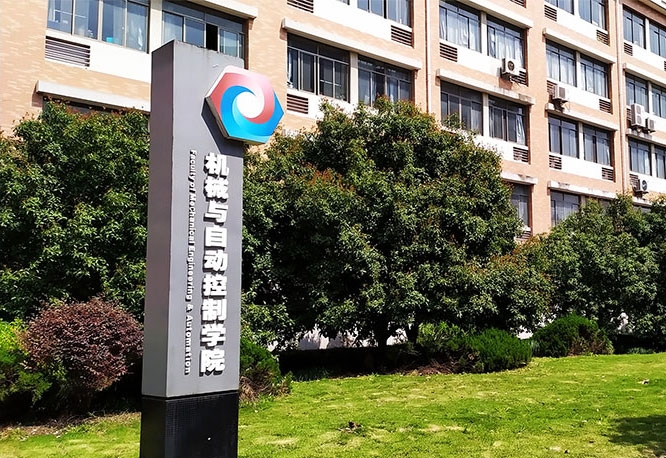
\includegraphics[scale=0.08]{nwafulogo/nwafu_logo_cie}}\\ %插入学院 logo
测控技术与仪器系\\
机械与自动控制学院\\
浙江理工大学 ] % 可选项,在每页边栏的底部显示
{% 显示在标题页
  测控技术与仪器系 \\
  机械与自动工程学院
  %西北农林科技大学\\
  %中国$\boldsymbol{\cdot}$杨凌
  
  % 在此要有一个空行,否则会在大学和国家之间产生额外的空白(I do not
  % 不知道为什么;( )
}

\date{\tosemester}

% 打开PDF后直接全屏
% \hypersetup{pdfpagemode={FullScreen}}
% ==================================================

% 设定仅编译的帧,加快编译速度
%\includeonlyframes{testframe}

% 定义章选择命令
\newcommand\seledchap[1]{%
  \ifcase#1\relax
  %\or
    \lecture{个人简介}{lec:introduction}
\section[课程概况]{课程概况及要求}\label{sec:chap00-sec02}
%%%%%%%%%%%%%%%%%%%%%%%%%%%%%% 课程概况 %%%%%%%%%%%%%%%%%%%%%%%%%%%%%%%%%%%
\begin{frame}{课程概况}{预修课程和教材}
  \stretchon
  \begin{itemize}
  \item\hilite<1> {\bfseries 预修课程:}
    \begin{itemize}
    \item C语言程序设计(无法回避的\alert{指针})
    \item 高等数学(永远的\alert{根})
    \item 英语(要求不高,但你得\alert{不断用})
    \end{itemize}\pause         
  \item\hilite<2> {\bfseries 教材:}
    \begin{itemize}
    \item C++面向对象程序设计(第2版). 龚晓庆, 付丽娜, 朱新懿, 李康著. 北京:清华大学
      出版社. 2011.
    \end{itemize}
    \centering
    \includegraphics[height=0.4\textheight]{chap00/01textbook.jpg} %
  \end{itemize}
  \stretchoff
\end{frame}

\begin{frame}{课程概况}{参考资料}
  \stretchon
  \begin{itemize}
  \item\hilite<1> {\bfseries 参考资料:}    
    \begin{itemize}
    \item The C++ Programming Language, 4th Edition. Stroustrup,
      Bjarne. Addison-Wesley. 2013.
    \item C++ How to Program, 10th Edition. Paul Deitel, Harvey
      Deitel. Prentice Hall. 2016.
    \item Programming Abstractions in C++. Eric Roberts. Prentice Hall. 2013.
    \end{itemize}
    \centering
    \includegraphics[height=0.35\textheight]{chap00/03programming.jpg} %
    \quad \includegraphics[height=0.35\textheight]{chap00/CHTP.jpg} %
    \quad \includegraphics[height=0.35\textheight]{chap00/PAinCPP.jpg} %
  \end{itemize}
  \stretchoff
\end{frame}

\section[要求]{基本要求}\label{sec:chap00-sec03}
\begin{frame}{课程要求}{基本要求}
  \stretchon
  \begin{itemize}
  \item {\bfseries 考勤}(\alert{扣分制度})
    \begin{itemize}
    \item 课堂随机考勤
    \item 实验课随机考勤
    \end{itemize}
  \item  {\bfseries 成绩评定}
    \begin{itemize}
    \item 结业(期末)考试---\alert{60\%}
      \begin{itemize}
      \item 笔试(\alert{闭卷},拟定于16周)
      \end{itemize}
    \item 平时成绩---\alert{40\%}
      \begin{itemize}
      \item 考勤      
      \item 学习通作业
      \item 大作业(论文分析或采用面向对象方法开发一个实用小软件)
      \end{itemize}
    \end{itemize}
  \end{itemize}
  \stretchoff
\end{frame}

\section[内容]{讲授内容}\label{sec:chap00-sec04}
\begin{frame}{课程内容}{讲授内容}
  \stretchon
  %\renewcommand{\labelenumi}{[\arabic{enumi}]} %
  % \begin{enumerate}
  % \item 第~\chinese{enumi}~章~面向对象基础%
  % \item 第~\chinese{enumi}~章~C++语言概览%
  % \item 第~\chinese{enumi}~章~C++语言基础%    
  % \item 第~\chinese{enumi}~章~复合类型
  % \item 第~\chinese{enumi}~章~函数%
  % \item 第~\chinese{enumi}~章~类和对象%
  % \item 第~\chinese{enumi}~章~对象的初始化、复制和销毁
  % \item 第~\chinese{enumi}~章~运算符重载%
  % \item 第~\chinese{enumi}~章~组合与继承%
  % \item 第~\chinese{enumi}~章~虚函数与多态性%
  % \item 第~\chinese{enumi}~章~模板与泛型编程%
  % \item 第~\chinese{enumi}~章~标准库容器和算法%
  % \item 第~\chinese{enumi}~章~异常处理
  % \end{enumerate}
  % %\renewcommand{\labelenumi}{[\arabic{enumi}]} %
  \begin{enumerate}
  \item 第~1~章~面向对象基础%
  \item 第~2~章~C++语言概览%
  \item 第~3~章~C++语言基础%    
  \item 第~4~章~复合类型
  \item 第~5~章~函数%
  \item 第~6~章~类和对象%
  \item 第~7~章~对象的初始化、复制和销毁
  \item 第~8~章~运算符重载%
  \item 第~9~章~组合与继承%
  \item 第~10~章~虚函数与多态性%
  \item 第~11~章~模板与泛型编程%
  \item 第~12~章~标准库容器和算法%
  \item 第~13~章~异常处理
  \end{enumerate}
  \stretchoff
\end{frame}

\begin{frame}{课程内容}{知识体系}
  \stretchon
  \begin{itemize}
  \item 思维导图
  \end{itemize}
  \centering
    \includegraphics[height=0.8\textheight]{chap00/oopmindmap} %
  \stretchoff
\end{frame}

\begin{frame}{课程内容}{知识体系}
  \stretchon
  \begin{itemize}
  \item 学习路线
  \end{itemize}
  \centering
  \includegraphics[height=0.8\textheight]{chap00/studyscheme} %
  \stretchoff
\end{frame}

%%%%%%%%%%%%%%%%%%%%%%%%%%%%%% 关于我 %%%%%%%%%%%%%%%%%%%%%%%%%%%%%%%%%%%
\section[关于我]{关于我}
\subsection[联系方式]{联系方式}
\begin{frame}[fragile]{关于我}{联系方式}
  % colour options
  \definecolor{seplinecolour}{HTML}{357f2d} % green
  \definecolor{iconcolour}{HTML}{2f3142} % dark
  \definecolor{textcolour}{HTML}{2f3142} % dark
  \definecolor{jobtitlecolour}{HTML}{474a65} % light dark

  % define some lengths for internal spacing
  \newlength{\seplinewidth} \setlength{\seplinewidth}{2cm}
  \newlength{\seplineheight} \setlength{\seplineheight}{1pt}
  \newlength{\seplinedistance} \setlength{\seplinedistance}{0.3cm}
  \begin{center}
    \begin{tikzpicture}
      % name
      \matrix[every node/.style={anchor=center,font=\huge},anchor=center] (name) {
        \node{郭晓忠}; \\
        \node{\color{jobtitlecolour}\normalsize\textit{讲师}}; \\
      };
      % sep line 1
      \node[below=0.3\seplinedistance of name] (hl1) {};
      \draw[line width=\seplineheight,color=seplinecolour] (hl1)++(-\seplinewidth/2,0) -- ++(\seplinewidth,0);
      % contact info
      \matrix [below=\seplinedistance of hl1,%
               column 1/.style={anchor=center,color=iconcolour},%
               column 2/.style={anchor=west}] (contact) {
        \node{\faGlobe}; & \node{\url{https://segmentfault.com/u/spartajet}};\\
        \node{\faBuilding}; & \node{机械与自动控制学院};\\ 
        \node{\faEnvelope}; & \node{guoxiaozhong@zstu.edu.cn};\\
        \node{\faQq}; & \node{972469693};\\
        \node{\faPhone}; & \node{13911521287}; \\
        \node{\faGithub}; & \node{\url{https://github.com/spartajet/}}; \\
      };
      %sep line 2
      \node[below=\seplinedistance of contact] (hl2) {};
      \draw[line width=\seplineheight,color=seplinecolour] (hl2)++(-\seplinewidth/2,0) -- ++(\seplinewidth,0);
      % interests
      \matrix [below=\seplinedistance of hl2,
         every node/.style={anchor=center,font=\LARGE}]
         (interests) {
        \node{\faCode}; & \node{\faCoffee}; &
        \node{\faLock}; & \node{\faWrench}; &
        \node{\faCameraRetro}; \\
      };
      
    \end{tikzpicture}
  \end{center}
\end{frame}
%%%%%%%%%%%%%%%%%%%%%%%%%%%%%%%%%%%%%%%%%%%%%%%%%%%%%%%%%%%%%%%%%%%%%%%%%%

%%% Local Variables: 
%%% mode: latex
%%% TeX-master: "../main.tex"
%%% End: 
 % 绪论
  \or % 第1章
    \include{data/ch01} % 基础知识
  \or % 第2章
    \lecture{绪论}{lec:chap02}
\section[知识回顾]{知识回顾}\label{sec:chap02-sec00}
%%%%%%%%%%%%%%%%%%%%%%%%%%%%%% 知识回顾 %%%%%%%%%%%%%%%%%%%%%%%%%%%%%%%%%%
%\stretchon%和\stretchoff
\begin{frame}[t, fragile]{知识回顾}{面向对象的基本概念}
  \stretchon
  \begin{itemize}
  \item 对象、类及其特性%\hilite<1>
    \begin{itemize}
    \item 什么是对象
    \item 什么是类
    \item 四大特性(数据抽象 、封装、继承和多态)
    \end{itemize}
  \item 面向对象程序设计语言发展史    
  \item 基本C++程序
    \begin{itemize}
    \item \cppinttfts{cin} 和 \cppinttfts{cout}
    \item \cppinttfts{using namespace}
    \end{itemize}
  \end{itemize}
  \stretchoff
\end{frame}
%\stretchoff

\begin{frame}{知识回顾}{发展史}
  \stretchon
  \begin{itemize}
  \item 族谱(Family tree)    
  \end{itemize}
  \centering
      \scalebox{0.7}{
        \centering
        %\tikzstyle{block} = [rectangle, draw, text width=10em, text centered, rounded corners, minimum height=1.0em]
        \tikzset{box/.style={rectangle, draw=black, rounded corners}}
        \tikzset{boxgreen/.style={rectangle, draw=black, rounded corners,fill=green}} 
        \begin{tikzpicture}
          \node[box] (asm) {Assembler};
          \node[box] (for) [right=0.5 of asm] {Fortran};
          \node[box] (alg)  [right=0.5  of for] {Algol};
          \node[box] (bcp)  [right=0.5  of alg] {BCPL};
          \node[box] (pas)  [above=1  of bcp] {Pascal};
          \node[box] (sim) [below=1 of bcp] {Simula};
          \node[box] (c) [right=0.5 of bcp] {C};
          \node[box] (cpp) [right=0.5 of c] {C++};
          \node[box] (cpp0x) [right=0.5 of cpp] {C++0x};
          \node[box] (opas) [above=1 of cpp0x, right=3.1 of pas] {Object Pascal};
          \node[box] (lisp) [below=2.5 of alg] {Lisp};
          \node[box] (smt) [right=2.5 of lisp] {Smalltalk};
          \node[box] (jar) [below=2.5 of cpp0x, right=0.8 of smt] {Java};
          \node (endmain)  [right=0.5  of cpp0x] {};
          \node (endopas)  [right=0.5 of opas] {};
          \node (endjava)  [right=0.5  of jar] {};

          \draw[->] (asm) -- (for);
          \draw[->] (for) -- (alg);
          \draw[->] (alg) -- (bcp);
          \draw[->] ([xshift=0.2em]alg.east) |- (pas);
          \draw[->] ([xshift=0.2em]alg.east) |- (sim);
          \draw[->] (sim.east) -|  (cpp);
          %\draw[->] (alg) -- (pas);
          \draw[->] (bcp) -- (c);
          \draw[->] (c) -- (cpp);
          \draw[->] (cpp) -- (cpp0x);
          \draw[->] (cpp0x) -- (endmain);
          \draw[->] ([xshift=0.2em]cpp.east) |-  ([yshift=-0.3em]opas.west);
          \draw[->] ([xshift=0.2em]cpp.east) |- ([yshift=0.3em]jar.west);
          \draw[->] (pas) -- (opas);
          \draw[->] (opas) -- (endopas);
          \draw[->] (lisp) -- (smt);
          \draw[->] ([xshift=0.2em]sim.east) |- ([yshift=0.3em]smt.west);
          \draw[->] (smt) -- (jar);
          \draw[->] (jar) -- (endjava);
        \end{tikzpicture}
      }
  \stretchoff
\end{frame}

\begin{frame}[fragile]{知识回顾}{基本C++程序}
  \begin{spacing}{1.1}%stretchon
  \begin{itemize}
  \item Hello, your name!\\
    \begin{center}
      \begin{minipage}{0.45\linewidth}
        \cppfile{codes/chap01/ex01-01.cpp}
      \end{minipage}
    \end{center}
  \item 名字空间
    \begin{itemize}
    \item \cppinttfts{using namespace}
    \end{itemize}
  \item 文件后缀名
    \begin{itemize}
    \item Windows: \cppinttfts{.cpp}
    \item Unix/Linux: \cppinttfts{.cpp}, \cppinttfts{.cc} or \cppinttfts{.c}
    \end{itemize}
  \end{itemize}
  \end{spacing}%stretchoff
\end{frame}
%%%%%%%%%%%%%%%%%%%%%%%%%%%%%%%%%%%%%%%%%%%%%%%%%%%%%%%%%%%%%%%%%%%%%%%%%%

\section[对C的扩充]{C++对C的扩充}\label{sec:chap02-sec01}
%%%%%%%%%%%%%%%%%%%%%%%%%%%%%% C++对C的扩充 %%%%%%%%%%%%%%%%%%%%%%%%%%%%%%%
\begin{frame}{扩充}{C++对C的扩充}
  \stretchon
  \begin{itemize}
  \item 格式化输入输出
  \item 基本数据类型与表达式
  \item 控制结构
  \item 构造数据类型
  \item 函数
  \item 大型程序结构控制
  \end{itemize}
  \stretchoff
\end{frame} 
%%%%%%%%%%%%%%%%%%%%%%%%%%%%%%%%%%%%%%%%%%%%%%%%%%%%%%%%%%%%%%%%%%%%%%%%%%

\section[输入输出]{格式化输入输出}\label{sec:chap02-sec02}
\subsection[cin/cout]{cin/cout}
%%%%%%%%%%%%%%%%%%%%%%%%%%%%% 格式化输入输出 %%%%%%%%%%%%%%%%%%%%%%%%%%%%%%
\begin{frame}[fragile]{输入输出}{格式化}%label=testframe,
  \begin{itemize}
  \item \cppinline{cin/cout}
  \end{itemize}
  \begin{center}
    \begin{tikzpicture}[show background grid]
      \tiny
      \umlnote[text width=0.55\textwidth](code1) at (0, 0)
      {
        \cppfiletikz{codes/chap02/ex02-01.cpp}
      };
    \end{tikzpicture}
    \includegraphics[width=0.45\textwidth]{chap02/01cppoutput01}
  \end{center}
\end{frame}  

\subsection[格式控制]{格式控制}
\begin{frame}[fragile]{输入输出}{输出格式设置}%
  \begin{itemize}
  \item 格式控制
  \end{itemize}
  \begin{spacing}{1.8}
  \begin{center}
    \scriptsize
    \begin{tabular}{|c|l|l|}
      \hline
      操作符 & 作用 & 说明 \\
      \hline
      \cppinttscr{oct} & 数据以8进制形式输出 & \multirow{3}{2cm}{作用范
                                              围为后续输出的整数,对小数不起作用}\\
      \cline{1-2}
      \cppinttscr{dec} & 数据以10进制形式输出(默认) & \\
      \cline{1-2}
      \cppinttscr{hex} & 数据以16进制形式输出 & \\
      \hline
      \cppinttscr{endl} & 换行并刷新输出流 & \\
      \hline
      \cppinttscr{setw(n)} & 设置输出宽度 & \multirow{2}{2cm}{作用范围为后续对象}\\
      \cline{1-2}
      \cppinttscr{setprecision(n)} & 设置输出精度(默认为6) & \\
      \hline
    \end{tabular}
    \begin{minipage}{0.65\linewidth}
      \scriptsize
      \begin{alertblock}{注意:}
        \begin{itemize}
        \item \cppinttscr{#include <iomanip>}
        \item 默认情况下, \cppinttscr{setprecision(n)}仅对带有小
          数的数有效, n为整数与小数位数之和
        \end{itemize}
      \end{alertblock}
    \end{minipage}
  \end{center}
  \end{spacing}
\end{frame}

\begin{frame}[fragile]{输入输出}{输出格式设置}%label=testframe,
  \begin{itemize}
  \item 设置输出格式
  \end{itemize}
  \begin{center}
    \begin{tikzpicture}[show background grid]
      \tiny
      \umlnote[scale=0.95, text width=0.55\textwidth](code1) at (0, 0)
      {
        \cppfiletikz{codes/chap02/ex02-02.cpp}
      };
    \end{tikzpicture}
    \includegraphics[width=0.45\textwidth]{chap02/01cppoutput02}
  \end{center}
\end{frame}  

  
%%%%%%%%%%%%%%%%%%%%%%%%%%%%%%%%%%%%%%%%%%%%%%%%%%%%%%%%%%%%%%%%%%%%%%%%%% 

\section[类型与表达式]{基本数据类型与表达式}\label{sec:chap02-sec03}
\subsection[基本类型]{基本类型}
\begin{frame}[t, fragile]{类型与表达式}{基本数据类型}
  \stretchon
  \begin{itemize}
  \item 基本数据类型
    \begin{itemize}
    \item \cppinttfts{int}, \cppinttfts{float}, \cppinttfts{double}, \cppinttfts{void}, \cppinttfts{char}
    \item 布尔型:\cppinttfts{bool} (\cppinttfts{true}$\Rightarrow$1, \cppinttfts{false}$\Rightarrow$0)
    \end{itemize}
  \item 变量与常量
    \begin{itemize}
    \item 变量的定义与赋初值
      \begin{itemize}
      \item \cppinttscr{int sum=100; double pi=3.1416; char c='a';}
      \item \cppinttscr{int sum(100); double pi(3.1416); char c('a');}
      \end{itemize}
    \item 符号常量与常变量
      \begin{itemize}
      \item \cppinttscr{#define PI 3.1416}
      \item \cppinttscr{const float PI=3.1416;}
      \item \cppinttscr{PI = 3.1415926535898;      // 错误!}
      \end{itemize}
    \end{itemize}
  \end{itemize}
  \stretchoff
\end{frame}

\subsection[新类型]{C++新类型}
\begin{frame}[fragile]{类型与表达式}{C++11中的新类型}
  \stretchon
  \begin{itemize}
  \item 常量表达式\\
  %\begin{center}
    \begin{minipage}{0.85\linewidth}
      \begin{cppcode}
const int size = 20;          // size是常量表达式
const int limits = size + 1;  // limits是常量表达式
int max = 80;                 // max不是常量表达式,80是字面值常量,
                              // 但max不是const, 不保证运行是不变。
const int lines = get_size(); // lines不是常量表达式
                              // lines是常量,但get_size()运行时才能确定
      \end{cppcode}
    \end{minipage}
  %\end{center}
  \item  \cppinline{constexpr}类型(验证是不是常量表达式)\\
     \begin{minipage}{0.85\linewidth}
      \begin{cppcode}
constexpr int size = 20;           // 20是常量表达式
constexpr int limits = size + 10;  // size + 10是常量表达式
constexpr int max = length();      // 取决于length()函数是不是常量函数
      \end{cppcode}
    \end{minipage}
  \item \cppinline{constexpr}与\cppinline{const}\\
    \begin{minipage}{0.85\linewidth}
      \begin{cppcode}
constexpr int a = length(); // 必须在编译时能计算出length()返回值
const int b = length();     // b的值可以在运行时获得,之后不再改变
      \end{cppcode}
    \end{minipage}
  \end{itemize}
  \stretchoff
\end{frame}

\begin{frame}[fragile]{类型与表达式}{C++11中的新类型}
  \stretchon
  \begin{itemize}
  \item \cppinline{auto}类型说明符\\
  %\begin{center}
    \begin{minipage}{0.95\linewidth}
      \begin{cppcode}
auto x = 5;               // 5是int类型,x则是int类型
auto size = sizeof(int);  // size是表示内存字节数的类型
auto name = "world";      // name是保存字符串的类型
cout << "hello " << name; // 可以使用name
auto a;                   // 错误!没有初始值无法确定类型
auto r = 1, pi = 3.14;    // 错误!类型混淆
     \end{cppcode}
    \end{minipage}
  %\end{center}
  \item  \cppinline{decltype}类型指示符,\alert{返回操作数类型}\\
     \begin{minipage}{0.95\linewidth}
      \begin{cppcode}
decltype(sizeof(int)) size; // sizeof(int)结果的类型
const int ci = 0;           // 是常量表达式
decltype(ci) x = 1;         // const int 类型
decltype(f()) y = sum;      // 函数f()的返回值类型
      \end{cppcode}
    \end{minipage}
  \end{itemize}
  \stretchoff
\end{frame}

\subsection[运算符与表达式]{运算符与表达式}
\begin{frame}[fragile]{类型与表达式}{运算符与表达式}
  \begin{spacing}{1.3}
  \begin{itemize}
  \item 运算符与表达式
    \begin{itemize}
    \item 算术运算符:\cppinttfts{+(|正号|), -(|负号|), *, /, %(|取余|)}
    \item 关系运算符:\cppinttfts{>, <, >=, <=, ==, !=}
    \item 逻辑运算符:\cppinttfts[escapeinside=//]{!, &&, ||}
    \item 位运算符: \cppinttfts[escapeinside=//]{~, <<, >>, &, ^(/异或/), /|/}
    \item 赋值运算符:\cppinttfts{=, *=, /=, %=, +=, -=, |$\cdots$|}
    \item 递增递减运算符:\cppinttfts{++, --}
    \end{itemize}
  \end{itemize}
  \centering  
  \begin{minipage}{0.3\linewidth}
    \scriptsize
    \begin{gather*}
      ax^{2}+bx+c=0 \\
      x_{1,2}=\frac{-b \pm \sqrt{b^{2}-4ac}}{2a}
    \end{gather*}
  \end{minipage}\\
  \begin{minipage}{0.6\linewidth}
    \begin{cppcode}
if(abs(b * b - 4 * a * c) > 1.0e - 10)
{
    x1 = (-b + sqrt(b * b - 4 * a * c)) / (2 * a);
    x2 = (-b - sqrt(b * b - 4 * a * c)) / (2 * a);
}
    \end{cppcode}
  \end{minipage}
  
  \end{spacing}
\end{frame}
%%%%%%%%%%%%%%%%%%%%%%%%%%%%%%%%%%%%%%%%%%%%%%%%%%%%%%%%%%%%%%%%%%%%%%%%%%

\section[控制结构]{控制结构}\label{sec:chap02-sec04}
%%%%%%%%%%%%%%%%%%%%%%%%%% 控制结构 %%%%%%%%%%%%%%%%%%%%%%%%%%%%%
\subsection[基本结构]{基本结构}
\begin{frame}[t, fragile]{控制结构}{基本结构}
  \stretchon
  \begin{itemize}
  \item 判断
    \begin{itemize}
    \item \cppinttfts{if ... else ...}
    \item \cppinttfts{if ... else if ... else ...}
    \item \cppinttfts{switch ... case ...}
    \end{itemize}
  \item 循环
    \begin{itemize}
    \item \cppinttfts{for(exp1;exp2;exp3){...}}
    \item \cppinttfts{while(exp){...}}
    \item \cppinttfts{do ... while(exp);}
    \end{itemize}
  \item 转移
    \begin{itemize}
    \item \cppinttfts{break}
    \item \cppinttfts{continue}
    \item \cppinttfts{goto}
    \end{itemize}
  \end{itemize}
  \stretchoff
\end{frame}

\subsection[范围for语句]{范围for语句}
\begin{frame}[fragile]{控制结构}{C++11中的范围for语句}
  \stretchon
  \begin{itemize}
  \item 范围\cppinline{for}语句\\[-1ex]
  %\begin{center}
    \begin{minipage}{0.95\linewidth}
      \begin{cppcode}
for(declaration : expression){
  statement;
}
// 其中:
//   expression必须是一个序列(列表、数组、vector、string等),
//     能返回begin和end对象。
//   declaration是一个变量,序列中每个元素都能够转换为该类型,
//     常用auto声明
      \end{cppcode}
    \end{minipage}
  %\end{center}
  \item 范围\cppinline{for}示例\\[-1ex]
     \begin{minipage}{0.95\linewidth}
      \begin{cppcode}
// 累加20以内的素数
int sum = 0;
for(int e : {2, 3, 5, 7, 11, 13, 17, 19}) // 用auto类型更合理
    sum += e;
cout << sum << endl;                      // 输出结果77
int arr[] = {1, 3, 5, 7, 9};              // 声明数组arr,初始化为5个奇数
for(auto ele : arr){                      // 声明ele,与数组arr关联在一起,用了auto
  ele = ele * 2;                          // 修改数组每个元素的值
  cout << ele << " ";                     // 输出ele,2 6 10 14 18
}
cout << endl;
for(auto ele : arr)
    cout << ele << " ";                   // 没有改变:1 3 5 7 9
cout << endl;
      \end{cppcode}
    \end{minipage}
  \end{itemize}
  \stretchoff
\end{frame}
%%%%%%%%%%%%%%%%%%%%%%%%%%%%%%%%%%%%%%%%%%%%%%%%%%%%%%%%%%%%%%%%%%%%%%%%%% 

\section[复杂类型]{复杂数据类型}\label{sec:chap02-sec05}
%%%%%%%%%%%%%%%%%%%%%%%%%%%%%%%% 构造数据类型 %%%%%%%%%%%%%%%%%%%%%%%%%%%%%%%%%%
% \begin{frame}[t, fragile]{复杂类型}{枚举和数组}
%   \stretchon
%   \begin{itemize}
%   \item 枚举类型
%     \begin{itemize}%\mintinline{c++}{}
%     \item \cppinline{enum weekday{SUN, MON,...,SAT};}
%     \end{itemize}
%   \item 数组
%     \begin{itemize}
%     \item 一维数组定义与初始化\\
%       \cppinline{int a[4]={1,2,3,4}; }\\
%       \cppinline{int a[]={1,2,3,4};}\\
%       \cppinline{char str[256]="movie.rm";}\\
%       \cppinline{char str[] = "movie.rm";}
%     \item 二维数组定义与初始化\\
%       \cppinline{int a[3][3]={{1,2,3},{4,5,6},{7,8,9}};}\\
%       \cppinline{int a[][3]={{1,2,3},{4,5,6},{7,8,9}};}
%     \end{itemize}  
%   \end{itemize}
%   \stretchoff
% \end{frame}
\subsection[指针与内存]{指针与内存}
\begin{frame}[t, fragile]{复杂类型}{指针}
  \begin{itemize}  
  \item 指针    
  \end{itemize}
  \hfill
  \begin{minipage}{0.35\linewidth}
    \begin{cppcode}    
int a=255;
int *p;
p=&a;
    \end{cppcode}
  \end{minipage}
  \begin{minipage}{0.6\linewidth}
    \tiny
    \begin{bytefield}{24}
      \begin{rightwordgroup}{\&a}
        \memsection[\&p$\rightarrow$]{0x00ff ffee}{0x00ff fffb}{4}{00FF 4212}
      \end{rightwordgroup}\\
      \memsection{}{}{4}{\ldots\ldots}\\
      \begin{rightwordgroup}{a}
        \memsection[\&a$\to$]{0x00ff 4212}{0x00ff 420f}{4}{0000 00FF}
      \end{rightwordgroup}\\
    \end{bytefield}
  \end{minipage}\\
  \begin{center}
    \begin{minipage}{0.7\linewidth}
      \begin{cppcode}      
float x[5];
float *p = x;
double sum = 0.0;
for (int i = 0; i < 5; i++)
{
  sum += *p++;
}      
      \end{cppcode}
    \end{minipage}
  \end{center}
\end{frame}

%\subsection[动态内存分配]{动态内存分配}
\begin{frame}[fragile]{复杂类型}{动态内存分配}
  \begin{itemize}
  \item 动态内存分配    
    \begin{itemize}
    \item \cppinttfts{malloc}和\cppinttfts{free}
    \item \cppinttfts{new}和\cppinttfts{delete}
    \end{itemize}  
  \end{itemize}
  \begin{center}
    \begin{minipage}{0.55\linewidth}
      \begin{cppcode}
// C语言
float *x = (float *)malloc(n*sizeof(float));
free (x);

// C++语言
float *x = new float[n];
delete []x;
      \end{cppcode}
    \end{minipage}\\%qquad
    \begin{minipage}{0.35\linewidth}
      \begin{cppcode}
int **mat;
int m, n;
mat = new int *[m];

for (i = 0; i < m; i++)
    mat[i] = new int[n];

for (i = 0; i < m; i++)
    delete [] mat[i];
delete [] mat;
      \end{cppcode}
    \end{minipage}
  \end{center}
\end{frame}
%\subsection[定位new表达式]{定位new表达式}
\begin{frame}[fragile]{复杂类型}{动态内存分配}
  \begin{itemize}
  \item 定位\cppinline{new}表达式
    \begin{itemize}
    \item 语法:\cppinttfts{new (|指针|)|类型|}
    \end{itemize}  
  \end{itemize}
  \begin{center}
    \begin{minipage}{0.7\linewidth}
      \begin{cppcode}
#include <iostream>
#include <new> // 必须包含该头文件

using namespace std;

char * buf = new char[1000]; // 预分配空间        

int main()
{
    int * pi = new (buf) int; // 在buf中创建一个int对象

    return 0;
}
      \end{cppcode}
    \end{minipage}
  \end{center}
\end{frame}

\subsection[指针与常量]{指针与常量}
\begin{frame}[t,fragile]{复杂类型}{指针常量和常量指针}
  \begin{itemize}
  \item 指针常量\\
    \begin{center}
      \begin{minipage}{0.6\linewidth}
        \begin{cppcode}
int a = 2, b = 3;
int * const p = &a;  //定义时必须赋初值
p = &b;              //错误,地址不能被修改
*p = b;              //正确,内容可以被修改
        \end{cppcode}
      \end{minipage}
    \end{center}
  \item 常量指针\\
    \begin{center}
      \begin{minipage}{0.55\linewidth}
        \begin{cppcode}
int a = 2, b = 3;
const int * p; 
p = &b;         //正确,地址可以被修改
*p = b;         //错误,内容不可以被修改
        \end{cppcode}
      \end{minipage}
    \end{center}
  \item 常指针常量\\
    \begin{center}
      \begin{minipage}{0.65\linewidth}
        \begin{cppcode}
int a = 2, b = 3;
const int * const p = &a;  //定义时必须赋初值
p = &b;         //错误,地址不能被修改
*p = b;         //错误,内容不可以被修改
        \end{cppcode}
      \end{minipage}
    \end{center}
  \end{itemize}
\end{frame}
\subsection[引用类型]{引用类型}
\begin{frame}[t, fragile]{复杂类型}{引用类型}
  \begin{itemize}
  \item 引用是已存在的变量的别名\\
    \begin{center}
      \begin{minipage}{0.6\linewidth}
        \begin{cppcode}
int i = 3;
int &j = i;   //引用必须赋初值
int &j = 3;   //错误,初值必须为变量
j = 4;
        \end{cppcode}
      \end{minipage}
    \end{center}
  \item 引用和指针的区别与联系\\
    \begin{center}
      \begin{minipage}{0.45\linewidth}
        \begin{cppcode}
int i = 3;
int &j = i;
int *k = &i;
cout << &i << endl;
cout << &j << endl;
cout << &k << endl;
        \end{cppcode}
      \end{minipage}
      \begin{minipage}{0.5\linewidth}
        \tiny
        \begin{bytefield}{24}
          \memsection{$\cdots$}{}{1}{$\cdots$}\\
          \memsection[k$\rightarrow$]{0x0016 FDEC}{}{1}{0x0016 FE04}\\
          \memsection{$\cdots$}{}{1}{$\cdots$}\\
          \memsection[$\genfrac{}{}{0pt}{}{\texttt{i}}{\texttt{j}}\rightarrow$]{0x0016 FE04}{}{1}{0x0000 0003}\\
          \memsection{$\cdots$}{}{1}{$\cdots$}
        \end{bytefield}
      \end{minipage}
    \end{center}
  \end{itemize}
\end{frame}

\begin{frame}[t, fragile]{复杂类型}{引用类型}
  \begin{itemize}
  \item 引用作为函数参数(例1)\\[-0.5ex]
    \begin{center}
      \scalebox{0.8}{
        \begin{minipage}{0.5\linewidth}
          \cppfile[fontsize=\scriptsize]{codes/chap02/ex02-03.cpp}
        \end{minipage}\qquad\qquad
        \begin{minipage}{0.5\linewidth}
          \cppfile[fontsize=\scriptsize]{codes/chap02/ex02-04.cpp}
        \end{minipage}
      }
    \end{center}
  \end{itemize}
\end{frame}

% \begin{frame}[t, label=testframe, fragile]{输出格式设置}%label=testframe,
%   \begin{center}
%     \begin{tikzpicture}[show background grid]
%       \tiny
%       \umlnote[text width=0.75\textwidth](code1) at (0, 0)
%       {
%         \cppfiletikz{codes/chap02/ex02-02.cpp}
%       };
%     \end{tikzpicture}
%     \includegraphics[width=0.5\textwidth]{chap02/01cppoutput02}
%   \end{center}
% \end{frame} 


\begin{frame}[t, fragile]{复杂类型}{引用类型}
  \begin{itemize}
  \item 引用作为函数参数(例2)\\
    \begin{center}
      \begin{minipage}{0.35\linewidth}
        \begin{cppcode}
struct StuNode
{
    int ID;
    char name[128];
    bool gender;
    int age;
    struct StuNode *next;
};
        \end{cppcode}
      \end{minipage}\qquad
      \begin{minipage}{0.5\linewidth}
        \begin{tikzpicture}[show background grid]
          \tiny
          \umlnote[text width = 0.85\textwidth](code1) at (0, 0)
          {
            \cppfiletikz{codes/chap02/ex02-05.cpp}
          };          
        \end{tikzpicture}        
        %\cppfile{codes/chap02/ex02-05.cpp}
      \end{minipage}
    \end{center}
  \end{itemize}
\end{frame}

\begin{frame}[t, fragile]{复杂类型}{引用类型}
  \begin{itemize}
  \item 引用作为函数参数(例2)\\
    \begin{center}
      \begin{minipage}{0.35\linewidth}
        \begin{cppcode}
struct StuNode
{
  int ID;
  char name[128];
  bool gender;
  int age;
  struct StuNode *next;
};
        \end{cppcode}
      \end{minipage}\qquad
      \begin{minipage}{0.5\linewidth}
        \begin{tikzpicture}[show background grid]
          \tiny
          \umlnote[text width = 0.85\textwidth](code1) at (0, 0)
          {
            \cppfiletikz{codes/chap02/ex02-06.cpp}
          };          
        \end{tikzpicture}
        %\cppfile{codes/chap02/ex02-06.cpp}
      \end{minipage}
    \end{center}
  \end{itemize}
\end{frame}

\begin{frame}[t,fragile]{复杂类型}{引用类型}
  \begin{itemize}
  \item 常引用\\
    \begin{minipage}{0.8\linewidth}
      \begin{cppcode}
int i = 100;
const int &r1 = 100;            //正确
const int &r2 = i;              //必须初始化
r2 = 200;                       //错误
      \end{cppcode}
    \end{minipage}
  \item 常引用参数\\
    \begin{minipage}{0.8\linewidth}
      \begin{cppcode}
int fun(const int &a, const int &b)
{
    return (a + b) / 2;         //参数不能被修改
}
      \end{cppcode}
    \end{minipage}
  \end{itemize}
\end{frame}

\begin{frame}[t,fragile]{复杂类型}{引用类型}
  \begin{itemize}
  \item 常引用\\
    \begin{minipage}{0.8\linewidth}
      \begin{cppcode}
int i = 100;
const int &r1 = 100;            //正确
const int &r2 = i;              //必须初始化
r2 = 200;                       //错误
      \end{cppcode}
    \end{minipage}
  \item 常引用参数\\
    \begin{minipage}{0.8\linewidth}
      \begin{cppcode}
int fun(const int &a, const int &b)
{
    return (a + b) / 2;         //参数不能被修改
}
      \end{cppcode}
    \end{minipage}
  \end{itemize}
\end{frame}
\subsection[C++类类型]{C++类类型}
\begin{frame}[fragile]{复杂类型}{迭代器}
  \begin{itemize}
  \item \cppinline{begin()}和\cppinline{end()}
    \begin{itemize}
    \item 语法\\
      \begin{center}
        \begin{minipage}{0.6\linewidth}
          \begin{cpptt}
begin(|\emph{数组名}|)
end(|\emph{数组名}|)
          \end{cpptt}
          \end{minipage}
      \end{center}
    \end{itemize}
  \item 运算
    \begin{itemize}
    \item 解引用
    \item 自增、自减
    \item 加或减整数、
    \item 指针相减
    \item 指针比较
    \end{itemize}
  \end{itemize}
  \begin{center}
    \begin{minipage}{0.6\linewidth}
      \begin{cppcode}
#include<iterator>  // 迭代器运算头文件
...
int ia[5] = {1, 2, 3, 4, 5};
int *pb = begin(ia);
int *pe = begin(ia);
while(pb != pe && *pb >= 0)
{
  ++pb;
}
      \end{cppcode}
    \end{minipage}
  \end{center}
\end{frame}
%\subsection[字符串]{字符串}
\begin{frame}[fragile]{复杂类型}{字符串}
  \stretchon
  \begin{itemize}
  \item 字符数组和C风格字符串
    \begin{itemize}
    \item 以\cppinttfts{'\0'}结束字符串
    \item 需要使用头文件:\cppinttfts{#include<cstring>}
    \end{itemize}
  \item C++的\cppinttfts{string}类
    \begin{itemize}
    \item 需要使用头文件:\cppinttfts{#include<string>}
    \item 丰富的字符串处理函数
    \item 便捷的运算符重载
    \item 单字符处理
      \begin{itemize}
      \item 需要使用头文件:\cppinttfts{#include<cctype>}
      \item 基本循环
      \item 范围for
      \end{itemize}
    \end{itemize}
  \end{itemize}
  \stretchoff
\end{frame}
%\subsection[vector向量]{vector向量}
\begin{frame}[fragile]{复杂类型}{向量}
  \stretchon
  \begin{itemize}
  \item 标准类型\cppinline{vector}
    \begin{itemize}
    \item 同种类型对象的集合
    \item 长度可变
    \end{itemize}
  \item 定义和初始化
    \begin{itemize}
    \item 语法:\cppinttfts{vector<|\emph{元素类型}|> |\emph{变量名}|;}
    \item 初始化方法\\[2ex]
      \tiny
      \begin{tabular}{l|l}
        %\scriptsize
        \toprule
        \multicolumn{1}{c|}{\emph{方 \qquad 法}} & \multicolumn{1}{c}{\emph{说 \qquad 明}} \\ \midrule
        \cppinttscr{vector<T> v1} & v1为空,元素是T类型,默认初始化 \\ \midrule
        \cppinttscr{vector<T> v2(v1)} & 声明v2向量,用v1初始化,是v1的副本 \\ \midrule
        \cppinttscr{vector<T> v2 = v1} & 等价于v2(v1) \\ \midrule
        \cppinttscr{vector<T> v3(n, val)} & v3有n个T类型的\alert{重复}元素,每个元素的值都是val\\ \midrule
        \cppinttscr{vector<T> v4(n)} & v4有n个\alert{重复}默认值初始化的元素 \\ \midrule
        \cppinttscr{vector<T> v5{a,b,c,...}} & v5元素个数为初始化式中元素个数 \\ \midrule
        \cppinttscr{vector<T> v5={a,b,c,...}} & 等价于v5\{a,b,c,...\} \\ \bottomrule
      \end{tabular}
    \end{itemize}
  \end{itemize}
  \stretchoff
\end{frame}
\subsection[类型转换]{类型转换}
\begin{frame}[fragile]{复杂类型}{类型转换}
  \stretchon
  \begin{itemize}
  \item 强制类型转换
    \begin{itemize}
    \item C风格\\
      \begin{cppcode}
float x = 3.5;
int roundX = (int)(x + 0.5);
      \end{cppcode}
    \item C++风格:\cppinttfts{castname<|\emph{类型名}|>(|\emph{表达式}|)}\\      
      \begin{itemize}
      \item \cppinttscr{static_cast}
      \item \cppinttscr{dynamic_cast}
      \item \cppinttscr{const_cast}
      \item \cppinttscr{reinterpret_cast}
      \end{itemize}
      \begin{cppcode}
int roundX = static_cast <int> (x+0.5);
      \end{cppcode}
    \end{itemize}
  \item 强制指针类型转换\\
    \begin{cppcode}
char *p;
void *q = malloc(sizeof(char)*1024);
p = q;    //错误!无法从“void *”转换为“char *”,C++
p =  (char *)q; 
    \end{cppcode}
  \end{itemize}
  \stretchoff
\end{frame}
%%%%%%%%%%%%%%%%%%%%%%%%%%%%%%%%%%%%%%%%%%%%%%%%%%%%%%%%%%%%%%%%%%%%%%%%%%

\section[函数]{函数}\label{sec:chap02-sec06}
%%%%%%%%%%%%%%%%%%%%%%%%%%%%%%%% 基本C++程序 %%%%%%%%%%%%%%%%%%%%%%%%%%%%%%%%%%
\begin{frame}{函数}{概述}
  \stretchon
  \begin{itemize}
  \item 函数调用执行过程
  \item 内联函数
  \item 带默认形参的函数
  \item 函数重载
  \item 函数模板
  \item 系统函数
  \end{itemize}
  \stretchoff
\end{frame}

\begin{frame}[fragile]{函数}{函数调用执行过程}
  \begin{itemize}
  \item 函数调用
    \begin{itemize}
    \item 参数和函数返回地址入栈
    \end{itemize}
  \item 执行函数体
    \begin{itemize}
    \item 寄存器进出栈,通过栈访问参数
    \end{itemize}
  \item 函数返回
    \begin{itemize}
    \item 返回到调用函数的下一条语句执行
    \end{itemize}
  \end{itemize}
  \begin{center}
    \begin{minipage}{0.3\linewidth}
      \begin{cppcode}
int increase(int a)
{
  return ++a;
}
int main()
{
  int x =3,y;
  y = increase(x);
  return 0;
}
      \end{cppcode}
    \end{minipage}
    \begin{minipage}{0.6\linewidth}
      \includegraphics[width=0.8\textwidth]{chap02/03funasm}
    \end{minipage}
  \end{center}
\end{frame}
\subsection[内联函数]{内联函数}
\begin{frame}[fragile]{函数}{内联函数}
  \stretchon
  \begin{itemize}
  \item 普通函数调用缺陷
    \begin{itemize}
    \item 时间开销
    \end{itemize}
  \item 内联函数
    \begin{itemize}
    \item 在编译时将函数体代码插入到调用处
    \item 适用于代码短、频繁调用的场合
    \end{itemize}
  \item 定义\\[2ex]
    %\begin{center}
      \begin{minipage}{0.6\linewidth}
        \begin{cpptt}
inline |函数类型| |函数名|(|参数表|)
{
    |函数体|;
}
       \end{cpptt}
      \end{minipage}
    %\end{center}
  \end{itemize}
  \stretchoff
\end{frame}

\begin{frame}[fragile]{函数}{内联函数}
  \begin{itemize}
  \item 本质是预处理后展开\\
    \begin{center}
      \begin{minipage}{0.4\linewidth}
        \begin{cppcode}
inline int increase(int a)
{
  return ++a;
}
int main()
{
  int x = 3,y;
  y = increase(x);
  return 0;
}
        \end{cppcode}
      \end{minipage}$\Longrightarrow$
      \begin{minipage}{0.3\linewidth}
        \begin{cppcode}
int main()
{
  int x = 3,y;
  int a = x;
  y = ++a;
  return 0;
}
        \end{cppcode}
      \end{minipage}
    \end{center}
  \item 效率测试\\
    \begin{center}
      \begin{minipage}{0.56\linewidth}
        \begin{cppcode}
inline float getCos_inline(int &x)
{
  float r;
  x = rand();
  r = cos(2 * 3.1416 * x / (float)RAND_MAX);
  return r;
}
        \end{cppcode}
      \end{minipage}
      \begin{minipage}{0.4\linewidth}
        \includegraphics[width=0.8\textwidth]{chap02/04inlinetest}\\
        \tiny
        测试环境 (Code:Blocks GCC Release)\\
        效率比 = 4057411ms/763214ms = 5.3
        \colorbox{yellow}{\textcolor{blue}{例02-07:ex02-07.cpp}}
      \end{minipage}
    \end{center}
  \end{itemize}
\end{frame}

\begin{frame}[fragile]{函数}{内联函数}
  \stretchon
  \begin{itemize}
  \item 注意事项
    \begin{itemize}
    \item 不能出现递归
    \item 代码不宜过长
    \item 不宜出现循环
    \item 不宜含有复杂控制语句如\cppinttfts{switch}等
    \item 有些编译器会智能处理是否为内联函数
    \end{itemize}
  \end{itemize}
  \stretchoff
\end{frame}
\subsection[constexpr函数]{constexpr函数}
\begin{frame}[fragile]{函数}{constexpr函数}
  \stretchon
  \begin{itemize}
  \item 语法
    \begin{itemize}
    \item \cppinttfts{constexpr |\emph{函数}|(|\emph{常量表达式函数}|)}
    \end{itemize}
  \item 基本要求
    \begin{itemize}
    \item 只有一句\cppinttfts{return}可执行语句,可有别名、
      \cppinttfts{using}等
    \item 必须有返回类型,返回类型不能是\cppinttfts{void}
    \item 使用前必须定义(不只是声明)
    \item \cppinttfts{return}中不能有非常量表达式
    \end{itemize}
  \end{itemize}
  \stretchoff
\end{frame}

\begin{frame}[fragile]{函数}{constexpr函数}
  \stretchon
  \begin{itemize}
  \item 是编译时求值,不是运行是调用\\[-1.5ex]
    \begin{cppcode}
constexpr int data() // 错误,函数体只能有一条return可执行语句
{
  const int i = 1;
  return i;
}
constexpr int data() // 正确
{
  return 1;
}
constexpr void f()   // 错误,无法获得常量
{
}
    \end{cppcode}
  \item 是函数使用(\alert{编译时}),不是函数调用(\alert{运行时})\\[-1.5ex]
    \begin{cppcode}
constexpr int f();     // 只有constexpr函数的声明,没有定义
int a = f();           // 正确,可以将编译时的计算转换为运行时的调用
const int b = f();     // 正确,编译器将f()转换为一个运行时的调用
constexpr int c = f(); // 错误,c是constexpr,要求使用f(),在编译时计算
constexpr int f()      // constexpr函数的定义
{
  return 1;
}
constexpr int d = f(); // 正确,f()已定义,可以使用f()
    \end{cppcode}
  \end{itemize}
  \stretchoff
\end{frame}

\begin{frame}[fragile]{函数}{constexpr函数}
  \stretchon
  \begin{itemize}
  \item \cppinline{return}中不能包含运行时才能确定的函数\\[-1.5ex]
    \begin{cppcode}
const int e() 
{        
  return 1;
}
constexpr int g()
{
  return e();     // 错误,调用了非constexpr函数
}
constexpr int e() 
{        
  return 1;
}
constexpr int g() 
{
  return e();     // 正确,函数e()是常量表达式函数
}
    \end{cppcode}
  \item 用\cppinline{constexpr}函数初始化\cppinline{constexpr}变量\\[-1.5ex]
    \begin{cppcode}
constexpr int new_sz()
{
  return 100;
}
constexpr int size = new_sz();
    \end{cppcode}
  \end{itemize}
  \stretchoff
\end{frame}
\subsection[形参默认值]{形参默认值}
\begin{frame}[fragile]{函数}{带默认形参值的函数}
  \begin{spacing}{1.8}
    \begin{itemize}
    \item 在函数定义或说明中\alert{为形参赋默认值}
    \item 作用
      \begin{itemize}
      \item 若调用给出实参值,则形参采用实参值
      \item 若调用未给出实参值,则调用默认参数值
      \end{itemize}
    \end{itemize}
  \end{spacing}
  \vspace{-2ex}
  \begin{center}
    \begin{minipage}{0.9\linewidth}
      \cppfile{codes/chap02/ex02-08.cpp}
    \end{minipage}
  \end{center}
\end{frame}

\begin{frame}[fragile]{函数}{带默认形参值的函数}
  \begin{spacing}{1.8}
    \begin{itemize}
    \item \alert{基本要求}
      \begin{itemize}
        \scriptsize
      \item 调用函数时,如省去某个实参,则该实参右边所有实参都要省略
      \item 默认形参必须\alert{自最右向左连续}定义
      \item 若函数声明(原型)中给出默认形参值,则函数定义时不能重复指定
      \end{itemize}
    \end{itemize}
  \end{spacing}
  \vspace{-3ex}
  \begin{center}
    \begin{minipage}{0.9\linewidth}
      \cppfile{codes/chap02/ex02-09.cpp}
    \end{minipage}
  \end{center}
\end{frame}

\begin{frame}[fragile]{函数}{带默认形参值的函数}
  \begin{itemize}
  \item \alert{中间参数不能省略}
  \end{itemize}
  \begin{center}
    \begin{minipage}{0.9\linewidth}
      \begin{tikzpicture}[show background grid]
        %\tiny
        \umlnote[text width = 1.00\textwidth](code1) at (0, 0)
        {
          \cppfiletikz{codes/chap02/ex02-10.cpp}
        };
      \end{tikzpicture}
      %\cppfile{codes/chap02/ex02-10.cpp}
    \end{minipage}
  \end{center}
\end{frame}

\begin{frame}[fragile]{函数}{带默认形参值的函数}
  \begin{itemize}
  \item \alert{不可重复指定参数默认值}
  \end{itemize}
  \begin{center}
    \begin{minipage}{0.9\linewidth}
      \cppfile{codes/chap02/ex02-11.cpp}
    \end{minipage}
  \end{center}
\end{frame}

\begin{frame}[fragile]{函数}{带默认形参值的函数}
  \begin{itemize}
  \item 默认形参必须\alert{自最右向左连续}定义
  \end{itemize}
  \begin{center}
    \begin{minipage}{0.9\linewidth}
      \cppfile{codes/chap02/ex02-12.cpp}
    \end{minipage}
  \end{center}
\end{frame}

\begin{frame}[fragile]{函数}{带默认形参值的函数}
  \begin{itemize}
  \item 默认形参必须\alert{自最右向左连续}定义
  \end{itemize}
  \begin{center}
    \begin{minipage}{0.9\linewidth}
      \cppfile{codes/chap02/ex02-13.cpp}
    \end{minipage}
  \end{center}
\end{frame}

\begin{frame}[fragile]{函数}{带默认形参值的函数}
  \begin{itemize}
  \item 必须为无默认值的参数提供实参
  \end{itemize}
  \begin{center}
    \begin{minipage}{0.9\linewidth}
      \begin{tikzpicture}[show background grid]
        %\tiny
        \umlnote[text width = 1.0\textwidth](code1) at (0, 0)
        {
          \cppfiletikz{codes/chap02/ex02-14.cpp}
        };
      \end{tikzpicture}
      %\cppfile{codes/chap02/ex02-14.cpp}
    \end{minipage}
  \end{center}
\end{frame}

\begin{frame}[fragile]{函数}{带默认形参值的函数}
  \begin{itemize}
  \item 形参的初始化可以是函数
  \end{itemize}
  \begin{center}
    \begin{minipage}{0.9\linewidth}
      \cppfile{codes/chap02/ex02-15.cpp}
    \end{minipage}
  \end{center}
\end{frame}
\subsection[重载函数]{重载函数}
\begin{frame}[fragile]{函数}{函数重载}
  \stretchon
  \begin{itemize}
  \item 重载:同一符号或函数名对应多种操作
    \begin{itemize}
    \item 操作符重载
    \item 函数重载
    \end{itemize}
  \item 函数重载
    \begin{itemize}
    \item 共性函数拥有相同函数名字\\
      \begin{cppcode}
int sum_int(int *a, int size);
float sum_float(float *a, int size);
double sum_double(double *a, int size);
      \end{cppcode}
      \vspace{-2ex}
      \begin{cppcode}
int sum(int *a, int size);
float sum(float *a, int size);
double sum(double *a, int size);
      \end{cppcode}
    \end{itemize}
  \end{itemize}
  \stretchoff
\end{frame}

\begin{frame}[fragile]{函数}{函数重载}
  \stretchon
  \begin{itemize}
  \item C++函数重载实现机理
    \begin{itemize}
    \item 函数名
    \item 参数类型
    \item 参数个数
    \end{itemize}
  \item 参数个数不同情况下的实现重载
    \begin{itemize}
      \begin{cppcode}
float dis_2d(float x0, float y0, float x1, float y1);
float dis_3d(float x0, float y0, float z0,
             float x1, float y1, float z1);
      \end{cppcode}
      \vspace{-2ex}
      \begin{cppcode}
float dis(float x0, float y0, float x1, float y1);
float dis(float x0, float y0, float z0,
          float x1, float y1, float z1);
      \end{cppcode}
    \end{itemize}
  \end{itemize}
  \stretchoff
\end{frame}

\begin{frame}[fragile]{函数}{函数重载}
  \stretchon
  \begin{itemize}
  \item 注意事项
    \begin{itemize}
    \item 避免二义性\\
      %\begin{center}
        \begin{minipage}{0.5\linewidth}
          \begin{cppcode}
void my_fun(int a, int b);
void my_fun(int &a, int &b);
          \end{cppcode}
        \end{minipage}
      %\end{center}
    \item 避免将不适宜重载的函数重载\\
      {\tiny 如果不同的函数名所提供的信息可使程序更容易理解,则不必使用重载}
      %\begin{center}
        \begin{minipage}{0.5\linewidth}
          \begin{cppcode}
void rotate(float r);
void translate(float x, float y);
          \end{cppcode}
          \vspace{-2ex}
          \begin{cppcode}
void transform(float r);
void transform(float x, float y);
          \end{cppcode}
        \end{minipage}
      %\end{center}
    \end{itemize}
  \end{itemize}
  \stretchoff
\end{frame}
\subsection{函数模板}
\begin{frame}[fragile]{函数}{函数模板}
  \stretchon
  \begin{itemize}
  \item 用一个函数表示逻辑功能相同但参数类型不同的函数\\
    %\begin{center}
      \begin{minipage}{0.6\linewidth}
        \begin{cppcode}
int sum(int *a, int size);
float sum(float *a, int size);
double sum(double *a, int size);
        \end{cppcode}
      \end{minipage}
    %\end{center}
  \item 定义\\
    %\begin{center}
      \tiny
      \begin{minipage}{0.8\linewidth}
        \mintinline{cpp}{template <class} 类型名1,
        \mintinline{cpp}{class} 类型名1, \ldots \mintinline{cpp}{>}
        返回类型~函数名(形参表)\\
        \{\\
            函数体;\\
        \}
      \end{minipage}\\
      \begin{minipage}{0.6\linewidth}
        \cppfile{codes/chap02/ex02-16.cpp}
      \end{minipage}
    %\end{center}
    \end{itemize}
  \stretchoff  
\end{frame}

\begin{frame}[fragile]{函数}{函数模板}
  \begin{itemize}  
  \item 带有两个通用类型的函数模板\\
    \begin{center}      
      \begin{minipage}{0.6\linewidth}
        \cppfile{codes/chap02/ex02-17.cpp}
      \end{minipage}
    \end{center}
  \end{itemize}
\end{frame}

\begin{frame}[fragile]{函数}{函数模板}
  \stretchon
  \begin{itemize}  
  \item 优先级别
    \begin{itemize}
    \item 如果同时定义重载函数,将优先使用重载函数,若不能找到精确匹配,再使用函数模板
    \end{itemize}
  \item 应用
    \begin{itemize}
    \item 数据结构中的链表、堆栈等
    \item C++的标准模板库(排序等)
    \item 通用类
    \end{itemize}
  \end{itemize}
  \stretchoff
\end{frame}

\begin{frame}[fragile]{函数}{函数模板}
  \begin{itemize}  
  \item 应用(例:冒泡排序)\\
    \begin{center}      
      \begin{minipage}{0.6\linewidth}
        \cppfile{codes/chap02/ex02-18.cpp}
      \end{minipage}
    \end{center}
  \end{itemize}
\end{frame}
\subsection{系统函数}
\begin{frame}[fragile]{函数}{系统函数}
  \stretchon
  \begin{itemize}  
  \item cmath
  \item iostream
    \begin{itemize}
    \item 包含\cppinttfts{ctype.h, string.h, memory.h, stdlib.h}等
        \cppinttfts{isdigit(), strcpy(), memcpy(), atoi(), rand()}等
    \end{itemize}
  \item ctime
    \begin{itemize}
    \item \cppinttfts{time_t, clock()}等
    \end{itemize}
  \end{itemize}
  \stretchoff
\end{frame}  
%%%%%%%%%%%%%%%%%%%%%%%%%%%%%%%%%%%%%%%%%%%%%%%%%%%%%%%%%%%%%%%%%%%%%%%%%%


\section[程序结构]{大型程序结构控制}\label{sec:chap02-sec07}
%%%%%%%%%%%%%%%%%%%%%%%%%%%%%%%% 基本C++程序 %%%%%%%%%%%%%%%%%%%%%%%%%%%%%%%%%%
\begin{frame}[fragile]{程序结构}{extern和static}
  \begin{itemize}  
  \item \cppinline{extern}    
    \begin{itemize}
      \tiny
    \item 大型程序设计中所有模块共同使用的全局变量(函数)
    \item 在一个模块中定义全局变量(函数),其它模块中
      用\cppinttscr{extern}说明``外来''的全局变量(函数)
    \end{itemize}
  \end{itemize}
  \vspace{-4.5ex}
  \begin{columns}
    \centering
    \begin{column}{0.42\textwidth}
      \centering
      \cppfile{codes/chap02/ex02-19-01.cpp}%}
      \vspace{-6ex}
      \cppfile{codes/chap02/ex02-19-02.cpp}%}
    \end{column}
    \begin{column}{0.42\textwidth}
      \centering
      \cppfile{codes/chap02/ex02-19-00.cpp}\\[-0.5ex]%}
      \includegraphics[width=0.8\textwidth]{chap02/05externkeyword}
    \end{column}
  \end{columns}
\end{frame}

\begin{frame}[fragile]{程序结构}{extern和static}
  \begin{itemize}  
  \item \cppinline{static}    
    \begin{itemize}
      \tiny
    \item \cppintttny{static}可用来声明全局静态变量和局部静态变量。当声明全局静态变
      量时,全局静态变量只能供本模块使用,不能被其它模块再声明
      为\cppintttny{extern}变量
    \end{itemize}
  \end{itemize}
  \begin{center}
    \begin{minipage}{0.4\linewidth}
      \cppfile{codes/chap02/ex02-20-01.cpp}
    \end{minipage}\qquad
    \begin{minipage}{0.4\linewidth}
      \cppfile{codes/chap02/ex02-20-02.cpp}
    \end{minipage}
  \end{center}
\end{frame}

\begin{frame}[fragile]{程序结构}{extern和static}
  \begin{itemize}  
  \item \cppinline{static}    
    \begin{itemize}
      \tiny
    \item 当一个局部变量声明为\cppintttny{static}变量,它既具有局部变量的性质,又具
      有全局变量的性质
    \end{itemize}
  \end{itemize}
  \begin{center}
    \begin{minipage}{0.53\linewidth}
      \cppfile{codes/chap02/ex02-21.cpp}
    \end{minipage}\qquad
    \begin{minipage}{0.35\linewidth}
      \includegraphics[width=0.8\textwidth]{chap02/06statickeyword}
    \end{minipage}
  \end{center}
\end{frame}

\begin{frame}[fragile]{程序结构}{包含头文件}
  \stretchon
  \begin{itemize}  
  \item 多文件操作使用\cppinline{#include}
  \item \cppintt{#include <|系统文件|>}
    \begin{itemize}
    \item 到编译器指定的文件包含目录查找
    \end{itemize}
  \item \cppintt{#include "|自定义文件.h"}
  \end{itemize}
  \stretchoff
\end{frame}

\begin{frame}[fragile]{程序结构}{条件编译}
  \begin{itemize}
  \item 同一程序在不同的编译条件下得到不同的目标代码
  \end{itemize}
  \begin{center}
    \begin{minipage}{0.6\linewidth}
      \cppfile{codes/chap02/ex02-22.cpp}
    \end{minipage}
  \end{center}
\end{frame}

\begin{frame}[fragile]{程序结构}{条件编译}
  \begin{itemize}
  \item 便于程序移植或跨平台
  \end{itemize}
  \begin{center}
    \begin{minipage}{0.4\linewidth}
      \cppfile{codes/chap02/ex02-23-01.cpp}
    \end{minipage}\qquad
    \begin{minipage}{0.4\linewidth}
      \cppfile{codes/chap02/ex02-23-02.cpp}
    \end{minipage}
  \end{center}
\end{frame}

\begin{frame}[fragile]{程序结构}{条件编译}
  \begin{itemize}
  \item 避免重复包含头文件如``MyHeader.h''\\
    \begin{center}
      \begin{minipage}{0.4\linewidth}
        \cppfile{codes/chap02/ex02-24.cpp}
      \end{minipage}
    \end{center}
  \item 便于调试程序\\
    \begin{center}
      \begin{minipage}{0.4\linewidth}
        \cppfile{codes/chap02/ex02-25.cpp}
      \end{minipage}
    \end{center}
  \end{itemize}
\end{frame}

\begin{frame}[fragile]{程序结构}{名字空间}
  \stretchon
  \begin{itemize}
  \item 不同程序员撰写的软件模块可能使用相同标志符
  \item 为避免冲突,将可能存在相同标志符的程序模块放入名字空间
  \item 定义:
    %\begin{center}
    \begin{minipage}{0.8\linewidth}
      \begin{cpptt}
namespace |名称|
{
   |成员变量或成员函数|;
}
        \end{cpptt}
      \end{minipage}
    %\end{center}    
    \end{itemize}
    \stretchoff
\end{frame}

\begin{frame}[fragile]{程序结构}{名字空间}
  \begin{itemize}
  \item 声明方式(作用域分辨符)\\
    名字空间名\cppinline{::}成员变量或成员函数\\
    \begin{center}
      \begin{minipage}{0.45\linewidth}
        \cppfile{codes/chap02/ex02-25-02.h}
      \end{minipage}\qquad
      \begin{minipage}{0.45\linewidth}
        \cppfile{codes/chap02/ex02-25-01.cpp}
      \end{minipage}
    \end{center}    
  \end{itemize}
\end{frame}

\begin{frame}[fragile]{程序结构}{名字空间}
  \begin{itemize}
  \item 声明方式(作用域分辨符) \\
    名字空间名\cppinline{::}成员变量或成员函数 \\
    \begin{center}
      \begin{minipage}{0.45\linewidth}
        \cppfile{codes/chap02/ex02-26-02.h}
      \end{minipage}\qquad
      \begin{minipage}{0.45\linewidth}
        \cppfile{codes/chap02/ex02-26-01.cpp}
      \end{minipage}
    \end{center}    
  \end{itemize}
\end{frame}
%%%%%%%%%%%%%%%%%%%%%%%%%%%%%%%%%%%%%%%%%%%%%%%%%%%%%%%%%%%%%%%%%%%%%%%%%%

% 附件页
\section[附件下载]{本讲示例代码及附件下载} 
\begin{frame}{附件}{本讲附件}
  % 此处的[ucfilespec=...]必须指定为pdf否则Windows下无法下载
  %\vspace{-4ex}
  \textattachfile[ucfilespec=ex-src02.pdf]{ex-src02.zip}{附件:右键单击该
    链接,选择\qtmark{\alert{保存附件}}下载,\alert{将后缀名改为\qtmark{.zip}解压}
      \footnote[frame]{请\alert{退出全屏模式}后点击该链接。}
      \footnote[frame]{以Adobe Acrobat Reader为例。}
      。}%\\

  \vspace{-1ex}
  \begin{center}
    \includegraphics[height=0.35\textheight]{pdfattatchdownload01}\quad
    %或 \quad%
    \includegraphics[height=0.35\textheight]{pdfattatchdownload02}\\[2ex]%
    \includegraphics[height=0.255\textheight]{pdfattatchdownload03}\quad
    %$\Rightarrow$ \quad%
    \includegraphics[height=0.255\textheight]{pdfattatchdownload04}%
  \end{center}   
\end{frame}

% \tiny
% \scriptsize
% \footnotesize
% \small
% \normalsize
% \large
% \Large
% \LARGE
% \huge
% \Huge


%%% Local Variables: 
%%% mode: latex
%%% TeX-master: "../main.tex"
%%% End: 
 % 算法
  \or % 第3章
    \include{data/ch03} % 输入/输出
  \or % 第4章
    \lecture{运算符重载}{lec:chap04}
\section[运算符重载]{从函数重载到运算符重载}\label{sec:chap04-sec01}
%%%%%%%%%%%%%%%%%%%%%%%%%%%%%% 从函数重载到运算符重载 %%%%%%%%%%%%%%%%%%%%%%%%%%%%%%%%%%
\begin{frame}[t, fragile]{运算符重载}{接口的多态性}%
  \begin{spacing}{1.8}
    \begin{itemize}
    \item 使用一致接口(uniform interface)处理不同数据
    \begin{itemize} 
    \item 函数重载 
    \item 运算符重载(``\cppinttfts{+}'')
      \begin{center}
        \begin{tikzpicture}[font=\tiny, show background grid]
          \umlnote[scale=1.0, text width=0.5\textwidth](note) {
            \begin{cppttnobg}
3.14 + 0.0015 = 3.1415;
[1, 2, 3] + [4, 5, 6] = [1, 2, 3, 4, 5, 6];
[3 + 4i] + [1 + 5i] = [4 + 9i];
"coffee" + " tea" = "coffee tea";
           \end{cppttnobg}
          };
        \end{tikzpicture}
      \end{center}
    \item 虚函数(继承与派生)
    \end{itemize}  
    \end{itemize}
  \end{spacing}
\end{frame}

\begin{frame}[t, fragile]{运算符重载}{函数重载的演化}%
  \stretchon
  \begin{itemize}
  \item 函数重载
    \begin{itemize}
    \item 功能相同、数据不同(类型或个数)的同名函数
    \end{itemize}
  \item 运算符重载
    \begin{itemize}
    \item 同一个运算符作用于不同类型数据的操作
    \item 运算符$\Rightarrow$ \alert{函数名}
    \end{itemize}
  \end{itemize}
  \stretchoff
\end{frame}

\begin{frame}[t, fragile]{运算符重载}{函数重载的演化}%
  \stretchon
  \begin{itemize}
  \item 运算符重载是C++的一大亮点
    \begin{itemize}
    \item 函数调用更简洁、直观
    \item 增加程序可读性(readability)
    \end{itemize}
  \item 实际应用
    \begin{itemize}
    \item 复数操作:\cppinttfts{(a+bi)+(c+di) = (a+c) + (b+d)i}
    \item 字符串操作:\cppinttfts{string1 == string2}
    \item 向量操作:\cppinttfts{(a1, |$\cdots$|, an)*s = (a1*s, |$\cdots$|, an*s)}
    \item 矩阵乘法:\cppinttfts{M = N*K}
    \item $\cdots$
    \end{itemize}
  \end{itemize}
  \stretchoff
\end{frame}

\begin{frame}[t, fragile]{运算符重载}{实例:经纬度类}%
  \begin{spacing}{1.5}
  \begin{itemize}
  \item 位置信息:纬度(latitude)和经度(longitude)
  \item 经纬度决定地球上一个地点的精确位置    
  \end{itemize}
  \begin{center}
    \begin{boxedminipage}{0.95\linewidth}
      \footnotesize      
      \heiti{已知:}

      \parindent=2em 北京天安门:(39.907306, 116.391264)

      \parindent=0em \heiti{求:}

      \parindent=2em 西南方向偏移(-5.642159, -8.323558)后的新位置?

      \parindent=0em \heiti{解:}

      \parindent=2em \fbox{\scriptsize \colorbox{green}{39.907306 + (- 5.642159)}}\quad\fbox{\scriptsize \colorbox{green}{116.391264 + (-
        8.323558)}}

      \parindent=0em \heiti{答案:}

      \parindent=2em    (34.265147 108.067706)$\Rightarrow$  西北农林科技大学行政楼位置
    \end{boxedminipage}
  \end{center}
  \end{spacing}
\end{frame}

\begin{frame}[t, fragile]{运算符重载}{实例:经纬度类}%
  \begin{spacing}{1.8}
  \begin{itemize}
  \item 位置信息:纬度(latitude)和经度(longitude)
  \item 经纬度决定地球上一个地点的精确位置    
  \end{itemize}  
  \begin{center}
    \begin{tabular}{ccc}
      \includegraphics[align=c,width=0.4\textwidth]{chap04/01tiananmen} & $\Rightarrow$ & \includegraphics[align=c,width=0.4\textwidth]{chap04/02nwsuaf}
    \end{tabular}
    %\includegraphics[width=0.45\textwidth]{chap04/01tiananmen}
    %\includegraphics[width=0.45\textwidth]{chap04/02nwsuaf}
  \end{center}
  \end{spacing}
\end{frame}

\begin{frame}[ t, fragile]{运算符重载}{实例:经纬度类}%
  \begin{itemize}
  \item 位置信息:纬度(latitude)和经度(longitude)
  \item 经纬度决定地球上一个地点的精确位置    
  \end{itemize}
  \begin{center}
    \begin{tikzpicture}[font=\tiny, show background grid]
      \tikzset{
        coord/.style={coordinate}
      }          
      \umlnote[scale=0.85, text width=0.55\textwidth](code1) at (0,0) {
        \cppfilettnobg{codes/chap04/ex04-01-01-CLocation.cpp}
      };
      \umlnote[scale=0.9, text width=0.52\textwidth](code2) at ($(code1.north) + (5.0, 0.0)$) {
        \cppfilettnobg{codes/chap04/ex04-01-02-main.cpp}
      };

      % Now we place the coordinate nodes for the connectors with
      % angles, or with annotations. , coord
      \node [coord] (c1) at ($(code1) + (-1.15, -1.20)$) {};
      \node [coord] (c2) at ($(code1) + (-0.4, -1.7)$) {};
      \node [coord] (c3) at ($(code2) + (-1.5, 0.5)$) {};
      \node [coord] (c4) at ($(code2) + (-1.5, 0.12)$) {};
      \node [coord] (c5) at ($(code2) + (-2.2, -1.00)$) {};  
    

      \node [draw, fill=blue!25] (note1) at ($(code1) +(1.0, 0)$)
      {\alert{+}运算符的重载};
      \node[draw, align=center, fill=blue!25] (note2) at ($(code2) +(1.2, 1.1)$)
      {北京天安门:\\(39.907306, 116.391264)};
      \node [draw, align=center, fill=blue!25] (note3) at ($(code2) +(1.2, -1.5)$)
      {西南方向偏移:\\(-5.642159, -8.323558)};
      \node [draw, align=center, fill=blue!25] (note4) at ($(code2) +(-0.8, -2.5)$)
      {西北农林科技大学\\行政楼位置};
      
      \draw[-{Stealth[scale=1.0]},red, thick] (note1.south)--(c1);
      \draw[-{Stealth[scale=1.0]},red, thick] (note1.south)--(c2);
      \draw[-{Stealth[scale=1.0]},red, thick] (note2.west)--(c3);
      \draw[-{Stealth[scale=1.0]},red, thick] (note3.north)--(c4);
      \draw[-{Stealth[scale=1.0]},red, thick] (note4.north)--(c5);
    \end{tikzpicture}
  \end{center}
\end{frame}
% %%%%%%%%%%%%%%%%%%%%%%%%%%%%%%%%%%%%%%%%%%%%%%%%%%%%%%%%%%%%%%%%%%%%%%%%%%%%%%%

\section[重载规则]{运算符重载规则}\label{sec:chap04-sec02}
%%%%%%%%%%%%%%%%%%%%%%%%%%%%%% 运算符重载规则 %%%%%%%%%%%%%%%%%%%%%%%%%%%%%%%%%%
\begin{frame}[t, fragile]{重载规则}{运算符重载规则}%
  \begin{spacing}{1.8}
  \begin{itemize}
  \item 可重载的运算符\\
    \begin{center}
      %\begin{minipage}{0.8\linewidth}
        \scriptsize
        \begin{tabular}{|c|c|c|c|c|c|c|c|c|}
          \hline
          \cppinttscr{+} & \cppinttscr{-} & \cppinttscr{*} & \cppinttscr{/} & \cppinttscr{%} & 
          \cppinttscr{^} & \cppinttscr{&} & \cppinline[fontsize=\scriptsize]{|} & \cppinttscr{~} \\

          \hline
          \cppinttscr{!} & \cppinttscr{,} & \cppinttscr{=} & \cppinttscr{<} & \cppinttscr{>} & 
          \cppinttscr{<=} & \cppinttscr{>=} & \cppinttscr{++} & \cppinttscr{--} \\

          \hline
          \cppinttscr{<<} & \cppinttscr{>>} & \cppinttscr{==} & \cppinttscr{!=} & \cppinttscr{&&} & 
          \cppinline[fontsize=\scriptsize]{||} & \cppinttscr{+=} & \cppinttscr{-=} & \cppinttscr{/=} \\

          \hline
          \cppinttscr{%=} & \cppinttscr{^=} & \cppinttscr{&=} & \cppinline[fontsize=\scriptsize]{|=} & \cppinttscr{*=} & 
          \cppinttscr{<<=} & \cppinttscr{>>=} & \cppinttscr{[]} & \cppinttscr{()} \\

          \hline
          \cppinttscr{->} & \cppinttscr{->*} & \cppinttscr{new} &
                                                               \cppinttscr{new []} & \cppinttscr{delete} & 
          \cppinttscr{delete []} &  &  & \\
          \hline
        \end{tabular}
      %\end{minipage}
    \end{center}
  \item 单目运算符和双目运算符
  \item 不可重载的运算符\\
    \begin{center}
      %\begin{minipage}{0.8\linewidth}
        \scriptsize
        \begin{tabular}{|c|c|c|c|}
          \hline
          \cppinttscr{.} & \cppinttscr{.*} & \cppinttscr{::} & \cppinttscr{?:}\\
          \hline
        \end{tabular}
      %\end{minipage}
    \end{center}
  \end{itemize}
  \end{spacing}
\end{frame}

\begin{frame}[t, fragile]{重载规则}{运算符重载规则}%
  \stretchon
  \begin{itemize}
  \item 重载规则
    \begin{itemize}
    \item 重载后运算符的优先级和结合性不变
    \item 运算符操作数的个数不能改变
    \item 不能重载C++中不支持的运算符 (@、\#、\$等)
    \item 保持运算符的语义%\\
      % \begin{tikzpicture}[font=\tiny, show background grid]
      %   \umlnote[text width=0.6\textwidth](note) at (0,0)
      %   {
      %     \begin{cppttnobg}
      %       bool operator!( const string &s1, const string &s2 )
      %       {
      %         return( strcmp( s1.c_str(), s2.c_str() ) != 0 );
      %       }
      %     \end{cppttnobg}
      %   };
      %   \node at (4.5, -1) {\Large \badmark};
      % \end{tikzpicture}
    \end{itemize}
  \end{itemize}
  \stretchoff
\end{frame}
% %%%%%%%%%%%%%%%%%%%%%%%%%%%%%%%%%%%%%%%%%%%%%%%%%%%%%%%%%%%%%%%%%%%%%%%%%%%%%%%

\section[重载方式]{运算符重载方式}\label{sec:chap04-sec03}
%%%%%%%%%%%%%%%%%%%%%%%%%%%%%% 运算符重载方式 %%%%%%%%%%%%%%%%%%%%%%%%%%%%%%%%%%
\begin{frame}[t, fragile]{重载方式}{运算符重载方式}%
  \begin{spacing}{1.8}
  \begin{itemize}
  \item 重载为类的成员函数
    \begin{itemize}
    \item 定义\\
      \begin{center}
        \begin{minipage}{0.8\linewidth}
          \begin{cpptt}
|返回类型| [|类名|::]operator |运算符|(|形参表|) {}
CLocation operator+(CLocation op2);
          \end{cpptt}
        \end{minipage}
      \end{center}
    \end{itemize}
  \item 重载为类的非成员函数(\alert{一般为友员函数})
    \begin{itemize}
    \item 定义\\
      \begin{center}
        \begin{minipage}{0.8\linewidth}
          \begin{cpptt}
friend |返回类型| operator |运算符|(|形参表|) {}
          \end{cpptt}
        \end{minipage}
      \end{center}
    \end{itemize}
  \end{itemize}
  \end{spacing}
\end{frame}

\begin{frame}[t, fragile]{重载方式}{重载为类的成员函数}%
  \begin{spacing}{1.6}
  \begin{itemize}
  \item 语法:\cppinlinett{|返回类型| [|类名|::]operator |运算符|(|形参表|) {}}
    \begin{itemize}
    \item 返回类型一般是一个对象
    \item 可以省略一个形参\\
      \begin{tikzpicture}[font=\tiny, show background grid]
        \umlnote[text width=0.5\textwidth](note) at (0,0)
        {
          \begin{cppttnobg}
CLocation operator+(CLocation op2);
CLocation operator-(CLocation op2);
CLocation operator=(CLocation op2);
CLocation operator++();
          \end{cppttnobg}
        };
      \end{tikzpicture}           
    \end{itemize}
  \end{itemize}
  \begin{center}
    \begin{minipage}{0.6\linewidth}
      \tiny
      注意:用成员函数实现+运算符重载,只有一个参数!\\
      \begin{cppcode}
CLocation loc1(30,100), loc2(5,4);
loc1 = loc1 + loc2;
      \end{cppcode}
      \\ \alert{另一参数通过this指针隐式传递!}
    \end{minipage}
  \end{center}
  \end{spacing}
\end{frame}

\begin{frame}[t, fragile]{重载方式}{实例:经纬度类}%
  \begin{itemize}
  \item 重载函数定义\\
    \begin{center}
      \begin{tikzpicture}[font=\tiny, show background grid]
        \tikzset{ coord/.style={coordinate} }
        \umlnote[text width=0.52\textwidth](code1) at (0,0)
        {
          \cppfilettnobg{codes/chap04/ex04-02-01-CLocation.cpp}
        };
        \umlnote[text width=0.33\textwidth](code2) at ($(code1.north) + (4.8,0)$)
        {
          \cppfilettnobg{codes/chap04/ex04-02-02-main.cpp}
        };

        % Now we place the coordinate nodes for the connectors with
        % angles, or with annotations. , coord
        \node [coord] (c1) at ($(code1) + (-3.2, -0.95)$) {};
        \node [coord] (c2) at ($(c1) + (1.4, 0)$) {};
        \node [coord] (c3) at ($(code1) + (-3.2, -2.2)$) {};
        \node [coord] (c4) at ($(c3) + (1.4, 0)$) {};
        \node [coord] (c5) at ($(code2) + (-1.85, -0.1)$) {};
        \node [coord] (c6) at ($(code1) + (0.1, -1.2)$) {};
        \node [coord] (c7) at ($(code2) + (-1.85, -0.8)$) {};
        \node [coord] (c8) at ($(code1) + (0.8, -0.2)$) {};
        \node [coord] (c9) at ($(code2) + (-1.85, -1.0)$) {};
        \node [coord] (c10) at ($(code1) + (0.8, 1.3)$) {};

        \node [draw, fill=blue!25] (note1) at ($(code1) + (1.2, -3.2)$)
      {利用\alert{*this}指针返回运算后的对象};

        \draw[blue, thick] (c1)--(c2);
        \draw[blue, thick] (c3)--(c4);
        \draw[-{Stealth[scale=1.0]},red, thick] (c5)--(c6);
        \draw[-{Stealth[scale=1.0]},red, thick] (c7)--(c8);
        \draw[-{Stealth[scale=1.0]},red, thick] (c9)--(c10);

        \draw[-{Stealth[scale=1.0]},blue, thick] (note1.west)--(c2);
        \draw[-{Stealth[scale=1.0]},blue, thick] (note1.west)--(c4);
      \end{tikzpicture}
    \end{center}
  \end{itemize}
\end{frame}

\begin{frame}[t, fragile]{重载方式}{前缀与后缀运算符}%
  \begin{spacing}{2.0}
  \begin{itemize}
  \item 前缀运算符:\cppinline{++i}, \cppinline{--i}\\
    \begin{center}
      \begin{minipage}{0.5\linewidth}
        \begin{cpptt}
CLocation operator++();
CLocation operator--();
        \end{cpptt}
      \end{minipage}
    \end{center}
  \item 后缀运算符:\cppinline{i++}, \cppinline{i--}\\
    \begin{center}
      \begin{minipage}{0.4\linewidth}
        \begin{cpptt}
CLocation operator++(|\tikzmark{a1}|int x|\tikzmark{a2}|);
CLocation operator--(|\tikzmark{a3}|int x|\tikzmark{a4}|);
        \end{cpptt}
      \end{minipage}\qquad
      \begin{boxedminipage}{0.4\linewidth}
        \tiny
        \tikzmark{a5}\alert{哑元参数},仅表示重载后缀运算符
      \end{boxedminipage}
    \end{center}
  \end{itemize}
  
\begin{tikzpicture}[overlay,remember picture]
    \draw[blue, thick] (pic cs:a1) -- (pic cs:a2);
    \draw[blue, thick] (pic cs:a3) -- (pic cs:a4);
    \draw[-{Stealth[scale=1]}, red, thick] (pic cs:a5) -- (pic cs:a2);
    \draw[-{Stealth[scale=1]}, red, thick] (pic cs:a5) -- (pic cs:a4);
  \end{tikzpicture}
  \end{spacing}
\end{frame}

\begin{frame}[t, fragile]{重载方式}{前缀与后缀运算符}%
  \begin{itemize}
  \item 前缀与后缀\\
    \begin{center}
      \begin{tikzpicture}[font=\tiny, show background grid]
        \tikzset{ coord/.style={coordinate} }
        \umlnote[text width=0.54\textwidth](code1) at (0,0)
        {
          \cppfilettnobg{codes/chap04/ex04-03-01-PrePost.cpp}
        };
        \umlnote[text width=0.33\textwidth](code2) at ($(code1.north) + (4.7,0)$)
        {
          \cppfilettnobg{codes/chap04/ex04-03-02-main.cpp}
        };

      %   % Now we place the coordinate nodes for the connectors with
      %   % angles, or with annotations. , coord
        \node [coord] (c1) at ($(code1) + (-3.3, -0.1)$) {};
        \node [coord] (c2) at ($(c1) + (1.4, 0)$) {};
        \node [coord] (c3) at ($(code1) + (-3.3, -2.21)$) {};
        \node [coord] (c4) at ($(c3) + (4.9, 0)$) {};
        \node [coord] (c5) at ($(code2) + (-1.85, -0.55)$) {};
        \node [coord] (c6) at ($(code1) + (-0.0, 0.9)$) {};
        \node [coord] (c7) at ($(code2) + (-1.85, -0.75)$) {};
        \node [coord] (c8) at ($(code1) + (0.0, -0.9)$) {};

        \node [draw, fill=blue!25] (note1) at ($(code1) + (-0.4, -0.35)$)
      {返回运算后的对象};

        \draw[blue, thick] (c1)--(c2);
        \draw[blue, thick] (c3)--(c4);
        \draw[-{Stealth[scale=1]},red, thick] (c5) to[out=180,in=-90] (c6);
        \draw[-{Stealth[scale=1]},red, thick] (c7) to[out=180,in=90] (c8);
        %\draw[-{Stealth[scale=1.0]},red, thick] (c7)--(c8);

        \draw[-{Stealth[scale=1]},blue, thick] (note1.west)--(c1);
        \draw[-{Stealth[scale=1]},blue, thick] (note1.south)--($(c3)!0.3!(c4) + (0, 0.2)$);
      \end{tikzpicture}
    \end{center}
  \end{itemize}
\end{frame}

\begin{frame}[t, fragile]{重载方式}{重载为类的友元函数}%
  \stretchon
  \begin{itemize}
  \item 语法:\cppinlinett{friend |返回类型| operator |运算符|(|形参表|) {}}
    \begin{itemize}
    \item 友元函数\alert{没有this指针},需给出所有传递参数
      \begin{cppcode}
friend CLocation operator+(CLocation op1,CLocation op2);
      \end{cppcode}
    \item 若使用单目运算符且修改成员数据,\alert{需使用引用传递}
      \begin{cpptt}
friend CLocation operator++(CLocation &op1);
friend CLocation operator++(CLocation &op1, int|\tikzmark{ax}| x);
      \end{cpptt}
      \vspace{4ex}
      \hfill \tikzmark{bx}\fbox{\tiny \alert{哑元参数表示后缀}}
    \end{itemize}
  \end{itemize}
  
\begin{tikzpicture}[overlay,remember picture]
    \draw[-{Stealth[scale=1.0]}, red, thick] (pic cs:bx) to[out=180, in=-90] (pic cs:ax);
  \end{tikzpicture}
  \stretchoff
\end{frame}

\begin{frame}[t, fragile]{重载方式}{重载为类的友元函数}%
  \begin{itemize}
  \item 重载为类的友元函数\\
    \begin{center}
      \begin{tikzpicture}[font=\tiny, show background grid]
        \tikzset{ coord/.style={coordinate} }
        \umlnote[text width=0.8\textwidth](note) at (0,0)
        {
          \cppfilettnobg{codes/chap04/ex04-04-friendop.cpp}
        };
      \end{tikzpicture}
    \end{center}
  \end{itemize}
\end{frame}

\begin{frame}[t, fragile]{重载方式}{重载为类的友元函数}%
  \stretchon
  \begin{itemize}
  \item 操作符左右为不同类型数据
    \begin{itemize}
    \item \cppinttfts{CLocation loc1;}\\
      \begin{minipage}{0.6\linewidth}
        \begin{cpptt}
loc1 = loc1 * 1.01; |$\cdots$(1)|
loc1 = 1.01 * loc1; |$\cdots$(2)\tikzmark{aa}|
        \end{cpptt}
      \end{minipage}
    \item 如何实现?
      \begin{itemize}
      \item \fbox{\tiny \alert{重载为类的成员函数无法实现!}}\tikzmark{bb}
      \end{itemize}
    \end{itemize}
  \end{itemize}
  
\begin{tikzpicture}[overlay,remember picture]
    \draw[-{Stealth[scale=1.0]}, red, thick] (pic cs:aa) to[out=0, in=0] (pic cs:bb);
  \end{tikzpicture}
  \stretchoff
\end{frame}

\begin{frame}[t, fragile]{重载方式}{重载为类的友元函数}%
  \begin{itemize}
  \item 操作符左右为不同类型数据\\
    \begin{center}
      \begin{tikzpicture}[font=\tiny, show background grid]
        \tikzset{ coord/.style={coordinate} }
        \umlnote[text width=0.49\textwidth](note) at (0,0)
        {
          \cppfilettnobg{codes/chap04/ex04-05-01-friendop.cpp}
        };
        \umlnote[text width=0.33\textwidth](note) at (4.6,0)
        {
          \cppfilettnobg{codes/chap04/ex04-05-02-main.cpp}
        };
      \end{tikzpicture}
    \end{center}
  \end{itemize}
\end{frame}

\begin{frame}[t, fragile]{重载方式}{两种重载方式的比较}%
  \stretchon
  \begin{itemize}
  \item 一般单目运算符重载为类的成员函数,双目运算符重载为类的友元函数
  \item \cppinline{=, (), [], ->}双目运算符不能重载为类的友元函数
  \item ``\cppinline{>>}''和``\cppinline{<<}''只能重载为类的友元函数
  \end{itemize}
  \stretchoff
\end{frame}
%%%%%%%%%%%%%%%%%%%%%%%%%%%%%%%%%%%%%%%%%%%%%%%%%%%%%%%%%%%%%%%%%%%%%%%%%%%%%%%

\section[典型运算符]{典型运算符重载}\label{sec:chap04-sec04}
%%%%%%%%%%%%%%%%%%%%%%%%%%%%%% 典型运算符重载 %%%%%%%%%%%%%%%%%%%%%%%%%%%%%%%%%%
\begin{frame}[t, fragile]{典型运算符}{典型运算符重载}%
  \stretchon
  \begin{itemize}
  \item ``\cppinline{>>}''和``\cppinline{<<}''\tikzmark{b} \hspace{4em} \fbox{\tiny
      \tikzmark{a} 只能以\alert{友元函数}方式重载}
  \item ``\cppinline{=}''\tikzmark{c}
  \item ``\cppinline{[]}''\tikzmark{d}
  \item ``\cppinline{()}''\tikzmark{e}
  \item ``\cppinline{->}''\tikzmark{f}
  \item ``\cppinline{new}''、``\cppinline{delete}''、
    ``\cppinline{new[]}''和``\cppinline{delete []}''
  \item ``\cppinline{,}''
  \end{itemize}
  \begin{tikzpicture} [remember picture, overlay]
    \draw[-{Stealth[scale=1.0]}, red, thick](pic cs:a) -- (pic cs:b);
    \draw[decorate, decoration={brace}]({pic cs:f}|-{pic
      cs:c})+(0,1em)--node[right, inner sep=1em]{\tiny\fbox{只能以\alert{成员
        函数}方式重载}}({pic cs:f}|-{pic cs:f});
  \end{tikzpicture}
  \stretchoff
\end{frame}

\begin{frame}[t, fragile]{典型运算符}{典型运算符重载}%
  \begin{itemize}
  \item 重载运算符``\cppinline{>>}''和``\cppinline{<<}''\\
    \begin{center}
      \begin{tikzpicture}[font=\tiny, show background grid]
        \tikzset{ coord/.style={coordinate} }
        \umlnote[text width=0.75\textwidth](note) at (0,0)
        {
          \cppfilettnobg{codes/chap04/ex04-06-01-io.cpp}
        };
      \end{tikzpicture}
    \end{center}
  \end{itemize}
\end{frame}

\begin{frame}[t, fragile]{典型运算符}{典型运算符重载}%
  \begin{itemize}
  \item 重载运算符``\cppinline{>>}''和``\cppinline{<<}''\\
    \begin{center}
      \begin{tikzpicture}[font=\tiny, show background grid]
        \tikzset{ coord/.style={coordinate} }        
        \umlnote[text width=0.7\textwidth](note) at (0,0)
        {
          \cppfilettnobg{codes/chap04/ex04-06-02-main.cpp}
        };
      \end{tikzpicture}
    \end{center}
  \end{itemize}
\end{frame}

\begin{frame}[t, fragile]{典型运算符}{典型运算符重载}%
  \begin{itemize}
  \item 重载运算符``\cppinline{=}''\\
    \begin{center}
      \begin{tikzpicture}[font=\tiny, show background grid]
        \tikzset{ coord/.style={coordinate} }        
        \umlnote[text width=0.4\textwidth, anchor=135](code1) at (0,0)
        {          
          \begin{cppttnobg}
ch_stack operator=(ch_stack & sObj)
{
  size = sObj.size;
  tp = sObj.tp;
  s = sObj.s;
}
          \end{cppttnobg}
        };
        \umlnote[text width=0.4\textwidth, anchor=135](code2) at ($(code1.north) + (2.5, 0)$)
        {          
          \begin{cppttnobg}
ch_stack operator=(ch_stack & sObj)
{
  if(s != NULL)
      free(s);
  size = sObj.size;
  tp = sObj.tp;
  s = NULL;
  if (size != 0)
  {
    s = new char[size];
    for (int i = 0; i <= tp; i++)
        s[i] = sObj.s[i];
  }
}
          \end{cppttnobg}
        };
        \node [coord](a1) at ($(code1) + (-2.45, -0.6)$) {};
        \node [coord](a2) at ($(a1) + (1.1, 0)$) {};
        \node [coord](b1) at ($(code2) + (-2.55, -0.18)$) {};
        \node [coord](b2) at ($(code2) + (-2.55, -1.35)$) {};
        
        \node[draw, fill=blue!25,anchor=west] (node1) at ($(code1) + (-1.5, -2.5)$)
        {\alert{浅拷贝}};
        \node[draw, fill=green!25,anchor=west, right=1.2 of node1] (node2)
        {\alert{深拷贝}};

        \draw[decorate, decoration={brace, mirror}, xshift=-4pt, yshift=0pt] (b1)
        -- (b2) node [coord,midway,xshift=-0.15cm](br) {};

        \draw [blue, thick] (a1) -- (a2);
        \draw [-{Stealth[scale=1.0]}, red, thick] (node1.north)
        to[out=90,in=0] (a2.east);

        \draw [-{Stealth[scale=1.0]}, red, thick] (node2.east)
        to[out=0,in=180] (br.west);
        
        \draw [red,thick,fill=green!25, fill opacity=0.2]
        ($(b1)+(-0.13cm, 0.1cm)$) rectangle ($(b2)+(3.05cm,-0.35cm)$);             
      \end{tikzpicture}
    \end{center}
  \end{itemize}
\end{frame}

\begin{frame}[t, fragile]{典型运算符}{典型运算符重载}%
  \begin{itemize}
  \item 自赋值检测\\
    \begin{center}
      \begin{tikzpicture}[font=\tiny, show background grid]
        \tikzset{ coord/.style={coordinate} }        
        \umlnote[text width=0.5\textwidth](note) at (0,0)
        {
          \begin{cppttnobg}
ClassName &ClassName::operator=(ClassName &s)
{
  if (this == &s)
      return *this;

  |$\cdots$|
}
          \end{cppttnobg}
        };        
      \end{tikzpicture}
    \end{center}    
  \item 引用计数与浅拷贝
    \begin{itemize}
    \item 深拷贝安全但某些情况下易浪费空间。
    \item 缺点:增加复杂度。
    \end{itemize}
  \end{itemize}
\end{frame}

\begin{frame}[t, fragile]{典型运算符}{典型运算符重载}%
  \begin{itemize}
  \item 重载运算符``\cppinline{[]}''
    \begin{itemize}
    \item 防止数组越界
    \end{itemize}
    \begin{center}
      \begin{tikzpicture}[font=\tiny, show background grid]
        \tikzset{ coord/.style={coordinate} }
        \umlnote[text width=0.45\textwidth](code1) at (0,0)
        {
          \cppfilettnobg{codes/chap04/ex04-07-01-index.cpp}
        };
        \umlnote[text width=0.35\textwidth](code2) at ($(code1.north) + (4.5,0)$)
        {
          \cppfilettnobg{codes/chap04/ex04-07-02-main.cpp}
        };

        \node [coord](b1) at ($(code1) + (-3.0, -0.25)$) {};
        \node [coord](b2) at ($(b1) + (3.8, -2.4)$) {};

        \draw [red,thick,fill=green!25, fill opacity=0.2]
        (b1) rectangle (b2);%($(b2)+(3.7cm, 0.0cm)$);  
      \end{tikzpicture}
    \end{center}
  \end{itemize}
\end{frame}

\begin{frame}[t, fragile]{典型运算符}{典型运算符重载}%
  \begin{itemize}
  \item 重载运算符``\cppinline{()}''
    \begin{itemize}
    \item 自动执行和表达式中的使用
    \item \alert{函数对象}
    \end{itemize}
    \begin{center}
      \begin{tikzpicture}[font=\tiny, show background grid]
        \tikzset{ coord/.style={coordinate} }
        \umlnote[text width=0.45\textwidth](code1) at (0,0)
        {
          \cppfilettnobg{codes/chap04/ex04-08-01-fun.cpp}
        };
        \umlnote[text width=0.35\textwidth](code2) at ($(code1.north) + (4.5,0)$)
        {
          \cppfilettnobg{codes/chap04/ex04-08-02-main.cpp}
        };

        %\node [coord](b1) at (-2.0, -2.45) {};
        %\node [coord](b2) at (-2.0, -4.35) {};
        \node [coord](b1) at ($(code1) + (-3.0, -0.35)$) {};
        \node [coord](b2) at ($(b1) + (4.0, -1.7)$) {};

        \node [coord](c1) at ($(code2) + (-2.15, -0.2)$) {};
        \node [coord](c2) at ($(c1) + (1.2, -0.35)$) {};

        \node [coord](c3) at ($(c1) + (1.22, -0.55)$) {};
        \node [coord](c4) at ($(c3) + (1.42, -0.35)$) {};
        

        \draw [red,thick,fill=green!25, fill opacity=0.2]
        (b1) rectangle (b2);

        \draw [red,thick,fill=green!25, fill opacity=0.2]
        (c1) rectangle (c2);

        \draw [red,thick,fill=green!25, fill opacity=0.2]
        (c3) rectangle (c4);
      \end{tikzpicture}
    \end{center}
  \end{itemize}
\end{frame}

\begin{frame}[t, fragile]{典型运算符}{典型运算符重载}%
  \begin{itemize}
  \item 重载运算符``\cppinline{->}''(\alert{应用于安全指针})    
    \begin{center}
      \begin{tikzpicture}[font=\tiny, show background grid]
        \tikzset{ coord/.style={coordinate} }
        \umlnote[text width=0.45\textwidth](note) at (0,0)
        {
          \begin{cppttnobg}
ClassName* ClassName::operator->();
          \end{cppttnobg}
        };
      \end{tikzpicture}
    \end{center}
  \end{itemize}
\end{frame}

\begin{frame}[t, fragile]{典型运算符}{典型运算符重载}%
  \begin{spacing}{1.6}
  \begin{itemize}
  \item 重载运算符``\cppinline{new}''和``\cppinline{delete}''
    \begin{itemize}
    \item 自定义的内存分配与释放(如在堆区无内存可分配的情况下自动使用
      磁盘空间)\\
      \begin{center}
      \begin{tikzpicture}[font=\tiny, show background grid]
        \tikzset{ coord/.style={coordinate} }
        \umlnote[text width=0.55\textwidth](note) at (0,0)
        {
          \begin{cppttnobg}
void *ClassName::operator new(size_t size);
void ClassName::operator delete(void *p);
          \end{cppttnobg}
        };
      \end{tikzpicture}
    \end{center}
  \item 使用系统的``\cppinline{new}''和``\cppinline{delete}''\\
    \begin{center}
      \begin{tikzpicture}[font=\tiny, show background grid]
        \tikzset{ coord/.style={coordinate} }
        \umlnote[text width=0.55\textwidth](note) at (0,0)
        {
          \begin{cppttnobg}
::new
::delete
          \end{cppttnobg}
        };
      \end{tikzpicture}
    \end{center}
    \end{itemize}    
  \end{itemize}
  \end{spacing}
\end{frame}

\begin{frame}[t, fragile]{典型运算符}{典型运算符重载}%
  \begin{spacing}{1.6}
  \begin{itemize}
  \item 重载运算符``\cppinline{new[]}''和``\cppinline{delete[]}''
    \begin{itemize}
    \item 为数组动态分配内存空间\\
      \begin{center}
        \begin{tikzpicture}[font=\tiny, show background grid]
          \tikzset{ coord/.style={coordinate} }
          \umlnote[text width=0.55\textwidth](note) at (0,0)
          {
            \begin{cppttnobg}
void *ClassName::operator new[](size_t size);
void ClassName::operator delete[](void *p);
            \end{cppttnobg}
          };
        \end{tikzpicture}
      \end{center}
    \end{itemize}
  \item 重载运算符``\cppinline{,}''\\
    \begin{center}
      \begin{tikzpicture}[font=\tiny, show background grid]
        \tikzset{ coord/.style={coordinate} }
        \umlnote[text width=0.55\textwidth](note) at (0,0)
        {
          \begin{cppttnobg}
ClassName ClassName::operator,(ClassName obj);
          \end{cppttnobg}
        };
      \end{tikzpicture}
    \end{center}
  \end{itemize}
  \end{spacing}
\end{frame}

\begin{frame}[t, fragile]{典型运算符}{典型运算符重载}%
  \begin{itemize}
  \item 类型转换运算符
    \begin{itemize}
    \item 重载``\cppinttfts{int}''、``\cppinttfts{float}''、$\cdots$(不必指定返回类型)
    \end{itemize}
    \begin{center}
      \begin{tikzpicture}[font=\tiny, show background grid]
        \tikzset{ coord/.style={coordinate} }
        \umlnote[text width=0.45\textwidth](note) at (0,0)
        {
          \begin{cppttnobg}
Rational r = 3.5f;
class Rational
{
  int up;
  int down;
public:
  //成员函数return
  operator float()
  {
    up/(float)down;
  }
};
          \end{cppttnobg}
        };
      \end{tikzpicture}
    \end{center}
  \end{itemize}
\end{frame}

\section[lambda函数]{lambda函数}
\begin{frame}[fragile]{lambda函数}{概述}%
  \stretchon
  \begin{itemize}
  \item 目的
    \begin{itemize}
    \item 将表达式传入函数(函数指针)
    \end{itemize}
  \item 本质
    \begin{itemize}
    \item 可调用的代码单元
    \item 类似于未命名的\cppinttfts{inline}函数
    \end{itemize}
  \item 实例
    \begin{cppcode}
#include <iostream>

using namespace std;

int main()
{
  int girls = 3, boys = 4;
  // lambda函数
  auto totalChild = [](int x, int y)->int {return x + y;};
  cout << totalChild(girls, boys) << endl;

  return 0;
}
   \end{cppcode}
  \item 别称
    \begin{itemize}
    \item \cppinline{lambda}表达式
    \end{itemize}
  \end{itemize}
  \stretchoff
\end{frame}

\begin{frame}[fragile]{lambda函数}{语法}%
  \begin{spacing}{1.5}
  \begin{itemize}
  \item 完整定义
    \begin{cppcode}
[capture list](params list) mutable exception -> return type{function body}
    \end{cppcode}
    \vspace{-4ex}
    \begin{description}
      \zihao{6}
    \item[\cppinttfts{capture list}] 捕获外部变量列表(上下文中的变量)
    \item[\cppinttfts{params list}] 形参列表

    \item[\cppinttfts{mutable}修饰符] 用于说明可否修改外部捕获的外部变量
    \item[\cppinttfts{exception}] 异常设定
    \item[\cppinttfts{return type}] 返回类型
    \item[\cppinttfts{function body}] 函数体  
    \end{description}
  \item 简化定义\\
    \begin{itemize}
      \zihao{6}
    \item \cppinttfts{[capture list](params list)->return type{function body}}
    \item \cppinttfts{[capture list](params list){function body}}
    \item \cppinttfts{[capture list]{function body}}
    \end{itemize}    
  \end{itemize}
  \end{spacing}
\end{frame}




\begin{frame}[t, fragile,allowframebreaks]{典型运算符}{运算符函数参数/
    返回类型}%
  \stretchon
  \begin{itemize}
  \item 对于任何参数类型,如果\alert{仅仅只是读参数}的值,应该作
    为\cppinline{const}引用来传递。普通算术运算符、关系运算符、逻辑运算
    符都不会改变参数,应该以\cppinline{const &}引用作为主要的参数传递方
    式。
  \item 当运算符函数是类的成员函数时,应该将其定义为\cppinline{const}成
    员函数。
  \item 返回值的类型取决于\alert{运算符的具体含义}。如果使用运算符的结
    果产生一个新值,就需要产生一个作为返回值的新对象,这个对象作为一个
    常量通过传值方式返回。
  \item \alert{如果函数返回的是原有对象,则通常以引用方式返回},根据是
    否希望对返回的值进行运算来决定是否返回\cppinline{const}引用。
  \item 所有赋值运算符均改变左值。为了使赋值结果能用于\alert{链式表达
      式},如\cppinline{a=b=c},应该返回一个改变了的左值的引用。一般赋
    值运算符的返回值是非\cppinline{const}引用,以便能够对刚刚赋值的对象
    进行运算。
  \end{itemize}
  \stretchoff
\end{frame}
%%%%%%%%%%%%%%%%%%%%%%%%%%%%%%%%%%%%%%%%%%%%%%%%%%%%%%%%%%%%%%%%%%%%%%%%%%%%%%%

% 附件页
\section[附件下载]{本讲示例代码及附件下载} 
\begin{frame}{附件}{本讲附件}
  % 此处的[ucfilespec=...]必须指定为pdf否则Windows下无法下载
  %\vspace{-4ex}
  \textattachfile[ucfilespec=ex-src04.pdf]{ex-src04.zip}{附件:右键单击该
    链接,选择\qtmark{\alert{保存附件}}下载,\alert{将后缀名改为\qtmark{.zip}解压}
      \footnote[frame]{请\alert{退出全屏模式}后点击该链接。}
      \footnote[frame]{以Adobe Acrobat Reader为例。}
      。}%\\

  \vspace{-1ex}
  \begin{center}
    \includegraphics[height=0.35\textheight]{pdfattatchdownload01}\quad
    %或 \quad%
    \includegraphics[height=0.35\textheight]{pdfattatchdownload02}\\[2ex]%
    \includegraphics[height=0.255\textheight]{pdfattatchdownload03}\quad
    %$\Rightarrow$ \quad%
    \includegraphics[height=0.255\textheight]{pdfattatchdownload04}%
  \end{center}   
\end{frame}

% \tiny
% \scriptsize
% \footnotesize
% \small
% \normalsize
% \large
% \Large
% \LARGE
% \huge
% \Huge


%%% Local Variables: 
%%% mode: latex
%%% TeX-master: "../main.tex"
%%% End: 
 % 数据类型
  \or % 第5章
    \include{data/ch05} % 运算符和表达式
  \or % 第6章
    \include{data/ch06} % 函数
  \or % 第7章
    \include{data/ch07} % 控制结构
  \or % 第8章
    \include{data/ch08} % 数组
  \or % 第9章
    \include{data/ch09} % 字符串
  \or % 第10章
    \include{data/ch10} % 结构体
  \or % 第11章
    \include{data/ch11} % 文件
  \or % 第12章
    \include{data/ch12} % 位运算及底层程序设计
  \fi
}

\begin{document}

%%%%%%%%%%%%%%%%%%%%%%%%%%%%%%%%%%%%%%%%%%%%%%%%%%%%%%%%%%%%%%%%% 
% 标题页
{\nwafuwavesbg%
  \begin{frame}[plain,noframenumbering] % plain选项移除标题页的边栏和页眉
    % \initclock % 启动时钟,若不需要,则注释该行
    \titlepage
  \end{frame}}
%%%%%%%%%%%%%%%%%%%%%%%%%%%%%%%%%%%%%%%%%%%%%%%%%%%%%%%%%%%%%%%%%
\seledchap{\chno}
% \lecture{个人简介}{lec:introduction}
\section[课程概况]{课程概况及要求}\label{sec:chap00-sec02}
%%%%%%%%%%%%%%%%%%%%%%%%%%%%%% 课程概况 %%%%%%%%%%%%%%%%%%%%%%%%%%%%%%%%%%%
\begin{frame}{课程概况}{预修课程和教材}
  \stretchon
  \begin{itemize}
  \item\hilite<1> {\bfseries 预修课程:}
    \begin{itemize}
    \item C语言程序设计(无法回避的\alert{指针})
    \item 高等数学(永远的\alert{根})
    \item 英语(要求不高,但你得\alert{不断用})
    \end{itemize}\pause         
  \item\hilite<2> {\bfseries 教材:}
    \begin{itemize}
    \item C++面向对象程序设计(第2版). 龚晓庆, 付丽娜, 朱新懿, 李康著. 北京:清华大学
      出版社. 2011.
    \end{itemize}
    \centering
    \includegraphics[height=0.4\textheight]{chap00/01textbook.jpg} %
  \end{itemize}
  \stretchoff
\end{frame}

\begin{frame}{课程概况}{参考资料}
  \stretchon
  \begin{itemize}
  \item\hilite<1> {\bfseries 参考资料:}    
    \begin{itemize}
    \item The C++ Programming Language, 4th Edition. Stroustrup,
      Bjarne. Addison-Wesley. 2013.
    \item C++ How to Program, 10th Edition. Paul Deitel, Harvey
      Deitel. Prentice Hall. 2016.
    \item Programming Abstractions in C++. Eric Roberts. Prentice Hall. 2013.
    \end{itemize}
    \centering
    \includegraphics[height=0.35\textheight]{chap00/03programming.jpg} %
    \quad \includegraphics[height=0.35\textheight]{chap00/CHTP.jpg} %
    \quad \includegraphics[height=0.35\textheight]{chap00/PAinCPP.jpg} %
  \end{itemize}
  \stretchoff
\end{frame}

\section[要求]{基本要求}\label{sec:chap00-sec03}
\begin{frame}{课程要求}{基本要求}
  \stretchon
  \begin{itemize}
  \item {\bfseries 考勤}(\alert{扣分制度})
    \begin{itemize}
    \item 课堂随机考勤
    \item 实验课随机考勤
    \end{itemize}
  \item  {\bfseries 成绩评定}
    \begin{itemize}
    \item 结业(期末)考试---\alert{60\%}
      \begin{itemize}
      \item 笔试(\alert{闭卷},拟定于16周)
      \end{itemize}
    \item 平时成绩---\alert{40\%}
      \begin{itemize}
      \item 考勤      
      \item 学习通作业
      \item 大作业(论文分析或采用面向对象方法开发一个实用小软件)
      \end{itemize}
    \end{itemize}
  \end{itemize}
  \stretchoff
\end{frame}

\section[内容]{讲授内容}\label{sec:chap00-sec04}
\begin{frame}{课程内容}{讲授内容}
  \stretchon
  %\renewcommand{\labelenumi}{[\arabic{enumi}]} %
  % \begin{enumerate}
  % \item 第~\chinese{enumi}~章~面向对象基础%
  % \item 第~\chinese{enumi}~章~C++语言概览%
  % \item 第~\chinese{enumi}~章~C++语言基础%    
  % \item 第~\chinese{enumi}~章~复合类型
  % \item 第~\chinese{enumi}~章~函数%
  % \item 第~\chinese{enumi}~章~类和对象%
  % \item 第~\chinese{enumi}~章~对象的初始化、复制和销毁
  % \item 第~\chinese{enumi}~章~运算符重载%
  % \item 第~\chinese{enumi}~章~组合与继承%
  % \item 第~\chinese{enumi}~章~虚函数与多态性%
  % \item 第~\chinese{enumi}~章~模板与泛型编程%
  % \item 第~\chinese{enumi}~章~标准库容器和算法%
  % \item 第~\chinese{enumi}~章~异常处理
  % \end{enumerate}
  % %\renewcommand{\labelenumi}{[\arabic{enumi}]} %
  \begin{enumerate}
  \item 第~1~章~面向对象基础%
  \item 第~2~章~C++语言概览%
  \item 第~3~章~C++语言基础%    
  \item 第~4~章~复合类型
  \item 第~5~章~函数%
  \item 第~6~章~类和对象%
  \item 第~7~章~对象的初始化、复制和销毁
  \item 第~8~章~运算符重载%
  \item 第~9~章~组合与继承%
  \item 第~10~章~虚函数与多态性%
  \item 第~11~章~模板与泛型编程%
  \item 第~12~章~标准库容器和算法%
  \item 第~13~章~异常处理
  \end{enumerate}
  \stretchoff
\end{frame}

\begin{frame}{课程内容}{知识体系}
  \stretchon
  \begin{itemize}
  \item 思维导图
  \end{itemize}
  \centering
    \includegraphics[height=0.8\textheight]{chap00/oopmindmap} %
  \stretchoff
\end{frame}

\begin{frame}{课程内容}{知识体系}
  \stretchon
  \begin{itemize}
  \item 学习路线
  \end{itemize}
  \centering
  \includegraphics[height=0.8\textheight]{chap00/studyscheme} %
  \stretchoff
\end{frame}

%%%%%%%%%%%%%%%%%%%%%%%%%%%%%% 关于我 %%%%%%%%%%%%%%%%%%%%%%%%%%%%%%%%%%%
\section[关于我]{关于我}
\subsection[联系方式]{联系方式}
\begin{frame}[fragile]{关于我}{联系方式}
  % colour options
  \definecolor{seplinecolour}{HTML}{357f2d} % green
  \definecolor{iconcolour}{HTML}{2f3142} % dark
  \definecolor{textcolour}{HTML}{2f3142} % dark
  \definecolor{jobtitlecolour}{HTML}{474a65} % light dark

  % define some lengths for internal spacing
  \newlength{\seplinewidth} \setlength{\seplinewidth}{2cm}
  \newlength{\seplineheight} \setlength{\seplineheight}{1pt}
  \newlength{\seplinedistance} \setlength{\seplinedistance}{0.3cm}
  \begin{center}
    \begin{tikzpicture}
      % name
      \matrix[every node/.style={anchor=center,font=\huge},anchor=center] (name) {
        \node{郭晓忠}; \\
        \node{\color{jobtitlecolour}\normalsize\textit{讲师}}; \\
      };
      % sep line 1
      \node[below=0.3\seplinedistance of name] (hl1) {};
      \draw[line width=\seplineheight,color=seplinecolour] (hl1)++(-\seplinewidth/2,0) -- ++(\seplinewidth,0);
      % contact info
      \matrix [below=\seplinedistance of hl1,%
               column 1/.style={anchor=center,color=iconcolour},%
               column 2/.style={anchor=west}] (contact) {
        \node{\faGlobe}; & \node{\url{https://segmentfault.com/u/spartajet}};\\
        \node{\faBuilding}; & \node{机械与自动控制学院};\\ 
        \node{\faEnvelope}; & \node{guoxiaozhong@zstu.edu.cn};\\
        \node{\faQq}; & \node{972469693};\\
        \node{\faPhone}; & \node{13911521287}; \\
        \node{\faGithub}; & \node{\url{https://github.com/spartajet/}}; \\
      };
      %sep line 2
      \node[below=\seplinedistance of contact] (hl2) {};
      \draw[line width=\seplineheight,color=seplinecolour] (hl2)++(-\seplinewidth/2,0) -- ++(\seplinewidth,0);
      % interests
      \matrix [below=\seplinedistance of hl2,
         every node/.style={anchor=center,font=\LARGE}]
         (interests) {
        \node{\faCode}; & \node{\faCoffee}; &
        \node{\faLock}; & \node{\faWrench}; &
        \node{\faCameraRetro}; \\
      };
      
    \end{tikzpicture}
  \end{center}
\end{frame}
%%%%%%%%%%%%%%%%%%%%%%%%%%%%%%%%%%%%%%%%%%%%%%%%%%%%%%%%%%%%%%%%%%%%%%%%%%

%%% Local Variables: 
%%% mode: latex
%%% TeX-master: "../main.tex"
%%% End: 

% \include{data/ch01}
% \lecture{绪论}{lec:chap02}
\section[知识回顾]{知识回顾}\label{sec:chap02-sec00}
%%%%%%%%%%%%%%%%%%%%%%%%%%%%%% 知识回顾 %%%%%%%%%%%%%%%%%%%%%%%%%%%%%%%%%%
%\stretchon%和\stretchoff
\begin{frame}[t, fragile]{知识回顾}{面向对象的基本概念}
  \stretchon
  \begin{itemize}
  \item 对象、类及其特性%\hilite<1>
    \begin{itemize}
    \item 什么是对象
    \item 什么是类
    \item 四大特性(数据抽象 、封装、继承和多态)
    \end{itemize}
  \item 面向对象程序设计语言发展史    
  \item 基本C++程序
    \begin{itemize}
    \item \cppinttfts{cin} 和 \cppinttfts{cout}
    \item \cppinttfts{using namespace}
    \end{itemize}
  \end{itemize}
  \stretchoff
\end{frame}
%\stretchoff

\begin{frame}{知识回顾}{发展史}
  \stretchon
  \begin{itemize}
  \item 族谱(Family tree)    
  \end{itemize}
  \centering
      \scalebox{0.7}{
        \centering
        %\tikzstyle{block} = [rectangle, draw, text width=10em, text centered, rounded corners, minimum height=1.0em]
        \tikzset{box/.style={rectangle, draw=black, rounded corners}}
        \tikzset{boxgreen/.style={rectangle, draw=black, rounded corners,fill=green}} 
        \begin{tikzpicture}
          \node[box] (asm) {Assembler};
          \node[box] (for) [right=0.5 of asm] {Fortran};
          \node[box] (alg)  [right=0.5  of for] {Algol};
          \node[box] (bcp)  [right=0.5  of alg] {BCPL};
          \node[box] (pas)  [above=1  of bcp] {Pascal};
          \node[box] (sim) [below=1 of bcp] {Simula};
          \node[box] (c) [right=0.5 of bcp] {C};
          \node[box] (cpp) [right=0.5 of c] {C++};
          \node[box] (cpp0x) [right=0.5 of cpp] {C++0x};
          \node[box] (opas) [above=1 of cpp0x, right=3.1 of pas] {Object Pascal};
          \node[box] (lisp) [below=2.5 of alg] {Lisp};
          \node[box] (smt) [right=2.5 of lisp] {Smalltalk};
          \node[box] (jar) [below=2.5 of cpp0x, right=0.8 of smt] {Java};
          \node (endmain)  [right=0.5  of cpp0x] {};
          \node (endopas)  [right=0.5 of opas] {};
          \node (endjava)  [right=0.5  of jar] {};

          \draw[->] (asm) -- (for);
          \draw[->] (for) -- (alg);
          \draw[->] (alg) -- (bcp);
          \draw[->] ([xshift=0.2em]alg.east) |- (pas);
          \draw[->] ([xshift=0.2em]alg.east) |- (sim);
          \draw[->] (sim.east) -|  (cpp);
          %\draw[->] (alg) -- (pas);
          \draw[->] (bcp) -- (c);
          \draw[->] (c) -- (cpp);
          \draw[->] (cpp) -- (cpp0x);
          \draw[->] (cpp0x) -- (endmain);
          \draw[->] ([xshift=0.2em]cpp.east) |-  ([yshift=-0.3em]opas.west);
          \draw[->] ([xshift=0.2em]cpp.east) |- ([yshift=0.3em]jar.west);
          \draw[->] (pas) -- (opas);
          \draw[->] (opas) -- (endopas);
          \draw[->] (lisp) -- (smt);
          \draw[->] ([xshift=0.2em]sim.east) |- ([yshift=0.3em]smt.west);
          \draw[->] (smt) -- (jar);
          \draw[->] (jar) -- (endjava);
        \end{tikzpicture}
      }
  \stretchoff
\end{frame}

\begin{frame}[fragile]{知识回顾}{基本C++程序}
  \begin{spacing}{1.1}%stretchon
  \begin{itemize}
  \item Hello, your name!\\
    \begin{center}
      \begin{minipage}{0.45\linewidth}
        \cppfile{codes/chap01/ex01-01.cpp}
      \end{minipage}
    \end{center}
  \item 名字空间
    \begin{itemize}
    \item \cppinttfts{using namespace}
    \end{itemize}
  \item 文件后缀名
    \begin{itemize}
    \item Windows: \cppinttfts{.cpp}
    \item Unix/Linux: \cppinttfts{.cpp}, \cppinttfts{.cc} or \cppinttfts{.c}
    \end{itemize}
  \end{itemize}
  \end{spacing}%stretchoff
\end{frame}
%%%%%%%%%%%%%%%%%%%%%%%%%%%%%%%%%%%%%%%%%%%%%%%%%%%%%%%%%%%%%%%%%%%%%%%%%%

\section[对C的扩充]{C++对C的扩充}\label{sec:chap02-sec01}
%%%%%%%%%%%%%%%%%%%%%%%%%%%%%% C++对C的扩充 %%%%%%%%%%%%%%%%%%%%%%%%%%%%%%%
\begin{frame}{扩充}{C++对C的扩充}
  \stretchon
  \begin{itemize}
  \item 格式化输入输出
  \item 基本数据类型与表达式
  \item 控制结构
  \item 构造数据类型
  \item 函数
  \item 大型程序结构控制
  \end{itemize}
  \stretchoff
\end{frame} 
%%%%%%%%%%%%%%%%%%%%%%%%%%%%%%%%%%%%%%%%%%%%%%%%%%%%%%%%%%%%%%%%%%%%%%%%%%

\section[输入输出]{格式化输入输出}\label{sec:chap02-sec02}
\subsection[cin/cout]{cin/cout}
%%%%%%%%%%%%%%%%%%%%%%%%%%%%% 格式化输入输出 %%%%%%%%%%%%%%%%%%%%%%%%%%%%%%
\begin{frame}[fragile]{输入输出}{格式化}%label=testframe,
  \begin{itemize}
  \item \cppinline{cin/cout}
  \end{itemize}
  \begin{center}
    \begin{tikzpicture}[show background grid]
      \tiny
      \umlnote[text width=0.55\textwidth](code1) at (0, 0)
      {
        \cppfiletikz{codes/chap02/ex02-01.cpp}
      };
    \end{tikzpicture}
    \includegraphics[width=0.45\textwidth]{chap02/01cppoutput01}
  \end{center}
\end{frame}  

\subsection[格式控制]{格式控制}
\begin{frame}[fragile]{输入输出}{输出格式设置}%
  \begin{itemize}
  \item 格式控制
  \end{itemize}
  \begin{spacing}{1.8}
  \begin{center}
    \scriptsize
    \begin{tabular}{|c|l|l|}
      \hline
      操作符 & 作用 & 说明 \\
      \hline
      \cppinttscr{oct} & 数据以8进制形式输出 & \multirow{3}{2cm}{作用范
                                              围为后续输出的整数,对小数不起作用}\\
      \cline{1-2}
      \cppinttscr{dec} & 数据以10进制形式输出(默认) & \\
      \cline{1-2}
      \cppinttscr{hex} & 数据以16进制形式输出 & \\
      \hline
      \cppinttscr{endl} & 换行并刷新输出流 & \\
      \hline
      \cppinttscr{setw(n)} & 设置输出宽度 & \multirow{2}{2cm}{作用范围为后续对象}\\
      \cline{1-2}
      \cppinttscr{setprecision(n)} & 设置输出精度(默认为6) & \\
      \hline
    \end{tabular}
    \begin{minipage}{0.65\linewidth}
      \scriptsize
      \begin{alertblock}{注意:}
        \begin{itemize}
        \item \cppinttscr{#include <iomanip>}
        \item 默认情况下, \cppinttscr{setprecision(n)}仅对带有小
          数的数有效, n为整数与小数位数之和
        \end{itemize}
      \end{alertblock}
    \end{minipage}
  \end{center}
  \end{spacing}
\end{frame}

\begin{frame}[fragile]{输入输出}{输出格式设置}%label=testframe,
  \begin{itemize}
  \item 设置输出格式
  \end{itemize}
  \begin{center}
    \begin{tikzpicture}[show background grid]
      \tiny
      \umlnote[scale=0.95, text width=0.55\textwidth](code1) at (0, 0)
      {
        \cppfiletikz{codes/chap02/ex02-02.cpp}
      };
    \end{tikzpicture}
    \includegraphics[width=0.45\textwidth]{chap02/01cppoutput02}
  \end{center}
\end{frame}  

  
%%%%%%%%%%%%%%%%%%%%%%%%%%%%%%%%%%%%%%%%%%%%%%%%%%%%%%%%%%%%%%%%%%%%%%%%%% 

\section[类型与表达式]{基本数据类型与表达式}\label{sec:chap02-sec03}
\subsection[基本类型]{基本类型}
\begin{frame}[t, fragile]{类型与表达式}{基本数据类型}
  \stretchon
  \begin{itemize}
  \item 基本数据类型
    \begin{itemize}
    \item \cppinttfts{int}, \cppinttfts{float}, \cppinttfts{double}, \cppinttfts{void}, \cppinttfts{char}
    \item 布尔型:\cppinttfts{bool} (\cppinttfts{true}$\Rightarrow$1, \cppinttfts{false}$\Rightarrow$0)
    \end{itemize}
  \item 变量与常量
    \begin{itemize}
    \item 变量的定义与赋初值
      \begin{itemize}
      \item \cppinttscr{int sum=100; double pi=3.1416; char c='a';}
      \item \cppinttscr{int sum(100); double pi(3.1416); char c('a');}
      \end{itemize}
    \item 符号常量与常变量
      \begin{itemize}
      \item \cppinttscr{#define PI 3.1416}
      \item \cppinttscr{const float PI=3.1416;}
      \item \cppinttscr{PI = 3.1415926535898;      // 错误!}
      \end{itemize}
    \end{itemize}
  \end{itemize}
  \stretchoff
\end{frame}

\subsection[新类型]{C++新类型}
\begin{frame}[fragile]{类型与表达式}{C++11中的新类型}
  \stretchon
  \begin{itemize}
  \item 常量表达式\\
  %\begin{center}
    \begin{minipage}{0.85\linewidth}
      \begin{cppcode}
const int size = 20;          // size是常量表达式
const int limits = size + 1;  // limits是常量表达式
int max = 80;                 // max不是常量表达式,80是字面值常量,
                              // 但max不是const, 不保证运行是不变。
const int lines = get_size(); // lines不是常量表达式
                              // lines是常量,但get_size()运行时才能确定
      \end{cppcode}
    \end{minipage}
  %\end{center}
  \item  \cppinline{constexpr}类型(验证是不是常量表达式)\\
     \begin{minipage}{0.85\linewidth}
      \begin{cppcode}
constexpr int size = 20;           // 20是常量表达式
constexpr int limits = size + 10;  // size + 10是常量表达式
constexpr int max = length();      // 取决于length()函数是不是常量函数
      \end{cppcode}
    \end{minipage}
  \item \cppinline{constexpr}与\cppinline{const}\\
    \begin{minipage}{0.85\linewidth}
      \begin{cppcode}
constexpr int a = length(); // 必须在编译时能计算出length()返回值
const int b = length();     // b的值可以在运行时获得,之后不再改变
      \end{cppcode}
    \end{minipage}
  \end{itemize}
  \stretchoff
\end{frame}

\begin{frame}[fragile]{类型与表达式}{C++11中的新类型}
  \stretchon
  \begin{itemize}
  \item \cppinline{auto}类型说明符\\
  %\begin{center}
    \begin{minipage}{0.95\linewidth}
      \begin{cppcode}
auto x = 5;               // 5是int类型,x则是int类型
auto size = sizeof(int);  // size是表示内存字节数的类型
auto name = "world";      // name是保存字符串的类型
cout << "hello " << name; // 可以使用name
auto a;                   // 错误!没有初始值无法确定类型
auto r = 1, pi = 3.14;    // 错误!类型混淆
     \end{cppcode}
    \end{minipage}
  %\end{center}
  \item  \cppinline{decltype}类型指示符,\alert{返回操作数类型}\\
     \begin{minipage}{0.95\linewidth}
      \begin{cppcode}
decltype(sizeof(int)) size; // sizeof(int)结果的类型
const int ci = 0;           // 是常量表达式
decltype(ci) x = 1;         // const int 类型
decltype(f()) y = sum;      // 函数f()的返回值类型
      \end{cppcode}
    \end{minipage}
  \end{itemize}
  \stretchoff
\end{frame}

\subsection[运算符与表达式]{运算符与表达式}
\begin{frame}[fragile]{类型与表达式}{运算符与表达式}
  \begin{spacing}{1.3}
  \begin{itemize}
  \item 运算符与表达式
    \begin{itemize}
    \item 算术运算符:\cppinttfts{+(|正号|), -(|负号|), *, /, %(|取余|)}
    \item 关系运算符:\cppinttfts{>, <, >=, <=, ==, !=}
    \item 逻辑运算符:\cppinttfts[escapeinside=//]{!, &&, ||}
    \item 位运算符: \cppinttfts[escapeinside=//]{~, <<, >>, &, ^(/异或/), /|/}
    \item 赋值运算符:\cppinttfts{=, *=, /=, %=, +=, -=, |$\cdots$|}
    \item 递增递减运算符:\cppinttfts{++, --}
    \end{itemize}
  \end{itemize}
  \centering  
  \begin{minipage}{0.3\linewidth}
    \scriptsize
    \begin{gather*}
      ax^{2}+bx+c=0 \\
      x_{1,2}=\frac{-b \pm \sqrt{b^{2}-4ac}}{2a}
    \end{gather*}
  \end{minipage}\\
  \begin{minipage}{0.6\linewidth}
    \begin{cppcode}
if(abs(b * b - 4 * a * c) > 1.0e - 10)
{
    x1 = (-b + sqrt(b * b - 4 * a * c)) / (2 * a);
    x2 = (-b - sqrt(b * b - 4 * a * c)) / (2 * a);
}
    \end{cppcode}
  \end{minipage}
  
  \end{spacing}
\end{frame}
%%%%%%%%%%%%%%%%%%%%%%%%%%%%%%%%%%%%%%%%%%%%%%%%%%%%%%%%%%%%%%%%%%%%%%%%%%

\section[控制结构]{控制结构}\label{sec:chap02-sec04}
%%%%%%%%%%%%%%%%%%%%%%%%%% 控制结构 %%%%%%%%%%%%%%%%%%%%%%%%%%%%%
\subsection[基本结构]{基本结构}
\begin{frame}[t, fragile]{控制结构}{基本结构}
  \stretchon
  \begin{itemize}
  \item 判断
    \begin{itemize}
    \item \cppinttfts{if ... else ...}
    \item \cppinttfts{if ... else if ... else ...}
    \item \cppinttfts{switch ... case ...}
    \end{itemize}
  \item 循环
    \begin{itemize}
    \item \cppinttfts{for(exp1;exp2;exp3){...}}
    \item \cppinttfts{while(exp){...}}
    \item \cppinttfts{do ... while(exp);}
    \end{itemize}
  \item 转移
    \begin{itemize}
    \item \cppinttfts{break}
    \item \cppinttfts{continue}
    \item \cppinttfts{goto}
    \end{itemize}
  \end{itemize}
  \stretchoff
\end{frame}

\subsection[范围for语句]{范围for语句}
\begin{frame}[fragile]{控制结构}{C++11中的范围for语句}
  \stretchon
  \begin{itemize}
  \item 范围\cppinline{for}语句\\[-1ex]
  %\begin{center}
    \begin{minipage}{0.95\linewidth}
      \begin{cppcode}
for(declaration : expression){
  statement;
}
// 其中:
//   expression必须是一个序列(列表、数组、vector、string等),
//     能返回begin和end对象。
//   declaration是一个变量,序列中每个元素都能够转换为该类型,
//     常用auto声明
      \end{cppcode}
    \end{minipage}
  %\end{center}
  \item 范围\cppinline{for}示例\\[-1ex]
     \begin{minipage}{0.95\linewidth}
      \begin{cppcode}
// 累加20以内的素数
int sum = 0;
for(int e : {2, 3, 5, 7, 11, 13, 17, 19}) // 用auto类型更合理
    sum += e;
cout << sum << endl;                      // 输出结果77
int arr[] = {1, 3, 5, 7, 9};              // 声明数组arr,初始化为5个奇数
for(auto ele : arr){                      // 声明ele,与数组arr关联在一起,用了auto
  ele = ele * 2;                          // 修改数组每个元素的值
  cout << ele << " ";                     // 输出ele,2 6 10 14 18
}
cout << endl;
for(auto ele : arr)
    cout << ele << " ";                   // 没有改变:1 3 5 7 9
cout << endl;
      \end{cppcode}
    \end{minipage}
  \end{itemize}
  \stretchoff
\end{frame}
%%%%%%%%%%%%%%%%%%%%%%%%%%%%%%%%%%%%%%%%%%%%%%%%%%%%%%%%%%%%%%%%%%%%%%%%%% 

\section[复杂类型]{复杂数据类型}\label{sec:chap02-sec05}
%%%%%%%%%%%%%%%%%%%%%%%%%%%%%%%% 构造数据类型 %%%%%%%%%%%%%%%%%%%%%%%%%%%%%%%%%%
% \begin{frame}[t, fragile]{复杂类型}{枚举和数组}
%   \stretchon
%   \begin{itemize}
%   \item 枚举类型
%     \begin{itemize}%\mintinline{c++}{}
%     \item \cppinline{enum weekday{SUN, MON,...,SAT};}
%     \end{itemize}
%   \item 数组
%     \begin{itemize}
%     \item 一维数组定义与初始化\\
%       \cppinline{int a[4]={1,2,3,4}; }\\
%       \cppinline{int a[]={1,2,3,4};}\\
%       \cppinline{char str[256]="movie.rm";}\\
%       \cppinline{char str[] = "movie.rm";}
%     \item 二维数组定义与初始化\\
%       \cppinline{int a[3][3]={{1,2,3},{4,5,6},{7,8,9}};}\\
%       \cppinline{int a[][3]={{1,2,3},{4,5,6},{7,8,9}};}
%     \end{itemize}  
%   \end{itemize}
%   \stretchoff
% \end{frame}
\subsection[指针与内存]{指针与内存}
\begin{frame}[t, fragile]{复杂类型}{指针}
  \begin{itemize}  
  \item 指针    
  \end{itemize}
  \hfill
  \begin{minipage}{0.35\linewidth}
    \begin{cppcode}    
int a=255;
int *p;
p=&a;
    \end{cppcode}
  \end{minipage}
  \begin{minipage}{0.6\linewidth}
    \tiny
    \begin{bytefield}{24}
      \begin{rightwordgroup}{\&a}
        \memsection[\&p$\rightarrow$]{0x00ff ffee}{0x00ff fffb}{4}{00FF 4212}
      \end{rightwordgroup}\\
      \memsection{}{}{4}{\ldots\ldots}\\
      \begin{rightwordgroup}{a}
        \memsection[\&a$\to$]{0x00ff 4212}{0x00ff 420f}{4}{0000 00FF}
      \end{rightwordgroup}\\
    \end{bytefield}
  \end{minipage}\\
  \begin{center}
    \begin{minipage}{0.7\linewidth}
      \begin{cppcode}      
float x[5];
float *p = x;
double sum = 0.0;
for (int i = 0; i < 5; i++)
{
  sum += *p++;
}      
      \end{cppcode}
    \end{minipage}
  \end{center}
\end{frame}

%\subsection[动态内存分配]{动态内存分配}
\begin{frame}[fragile]{复杂类型}{动态内存分配}
  \begin{itemize}
  \item 动态内存分配    
    \begin{itemize}
    \item \cppinttfts{malloc}和\cppinttfts{free}
    \item \cppinttfts{new}和\cppinttfts{delete}
    \end{itemize}  
  \end{itemize}
  \begin{center}
    \begin{minipage}{0.55\linewidth}
      \begin{cppcode}
// C语言
float *x = (float *)malloc(n*sizeof(float));
free (x);

// C++语言
float *x = new float[n];
delete []x;
      \end{cppcode}
    \end{minipage}\\%qquad
    \begin{minipage}{0.35\linewidth}
      \begin{cppcode}
int **mat;
int m, n;
mat = new int *[m];

for (i = 0; i < m; i++)
    mat[i] = new int[n];

for (i = 0; i < m; i++)
    delete [] mat[i];
delete [] mat;
      \end{cppcode}
    \end{minipage}
  \end{center}
\end{frame}
%\subsection[定位new表达式]{定位new表达式}
\begin{frame}[fragile]{复杂类型}{动态内存分配}
  \begin{itemize}
  \item 定位\cppinline{new}表达式
    \begin{itemize}
    \item 语法:\cppinttfts{new (|指针|)|类型|}
    \end{itemize}  
  \end{itemize}
  \begin{center}
    \begin{minipage}{0.7\linewidth}
      \begin{cppcode}
#include <iostream>
#include <new> // 必须包含该头文件

using namespace std;

char * buf = new char[1000]; // 预分配空间        

int main()
{
    int * pi = new (buf) int; // 在buf中创建一个int对象

    return 0;
}
      \end{cppcode}
    \end{minipage}
  \end{center}
\end{frame}

\subsection[指针与常量]{指针与常量}
\begin{frame}[t,fragile]{复杂类型}{指针常量和常量指针}
  \begin{itemize}
  \item 指针常量\\
    \begin{center}
      \begin{minipage}{0.6\linewidth}
        \begin{cppcode}
int a = 2, b = 3;
int * const p = &a;  //定义时必须赋初值
p = &b;              //错误,地址不能被修改
*p = b;              //正确,内容可以被修改
        \end{cppcode}
      \end{minipage}
    \end{center}
  \item 常量指针\\
    \begin{center}
      \begin{minipage}{0.55\linewidth}
        \begin{cppcode}
int a = 2, b = 3;
const int * p; 
p = &b;         //正确,地址可以被修改
*p = b;         //错误,内容不可以被修改
        \end{cppcode}
      \end{minipage}
    \end{center}
  \item 常指针常量\\
    \begin{center}
      \begin{minipage}{0.65\linewidth}
        \begin{cppcode}
int a = 2, b = 3;
const int * const p = &a;  //定义时必须赋初值
p = &b;         //错误,地址不能被修改
*p = b;         //错误,内容不可以被修改
        \end{cppcode}
      \end{minipage}
    \end{center}
  \end{itemize}
\end{frame}
\subsection[引用类型]{引用类型}
\begin{frame}[t, fragile]{复杂类型}{引用类型}
  \begin{itemize}
  \item 引用是已存在的变量的别名\\
    \begin{center}
      \begin{minipage}{0.6\linewidth}
        \begin{cppcode}
int i = 3;
int &j = i;   //引用必须赋初值
int &j = 3;   //错误,初值必须为变量
j = 4;
        \end{cppcode}
      \end{minipage}
    \end{center}
  \item 引用和指针的区别与联系\\
    \begin{center}
      \begin{minipage}{0.45\linewidth}
        \begin{cppcode}
int i = 3;
int &j = i;
int *k = &i;
cout << &i << endl;
cout << &j << endl;
cout << &k << endl;
        \end{cppcode}
      \end{minipage}
      \begin{minipage}{0.5\linewidth}
        \tiny
        \begin{bytefield}{24}
          \memsection{$\cdots$}{}{1}{$\cdots$}\\
          \memsection[k$\rightarrow$]{0x0016 FDEC}{}{1}{0x0016 FE04}\\
          \memsection{$\cdots$}{}{1}{$\cdots$}\\
          \memsection[$\genfrac{}{}{0pt}{}{\texttt{i}}{\texttt{j}}\rightarrow$]{0x0016 FE04}{}{1}{0x0000 0003}\\
          \memsection{$\cdots$}{}{1}{$\cdots$}
        \end{bytefield}
      \end{minipage}
    \end{center}
  \end{itemize}
\end{frame}

\begin{frame}[t, fragile]{复杂类型}{引用类型}
  \begin{itemize}
  \item 引用作为函数参数(例1)\\[-0.5ex]
    \begin{center}
      \scalebox{0.8}{
        \begin{minipage}{0.5\linewidth}
          \cppfile[fontsize=\scriptsize]{codes/chap02/ex02-03.cpp}
        \end{minipage}\qquad\qquad
        \begin{minipage}{0.5\linewidth}
          \cppfile[fontsize=\scriptsize]{codes/chap02/ex02-04.cpp}
        \end{minipage}
      }
    \end{center}
  \end{itemize}
\end{frame}

% \begin{frame}[t, label=testframe, fragile]{输出格式设置}%label=testframe,
%   \begin{center}
%     \begin{tikzpicture}[show background grid]
%       \tiny
%       \umlnote[text width=0.75\textwidth](code1) at (0, 0)
%       {
%         \cppfiletikz{codes/chap02/ex02-02.cpp}
%       };
%     \end{tikzpicture}
%     \includegraphics[width=0.5\textwidth]{chap02/01cppoutput02}
%   \end{center}
% \end{frame} 


\begin{frame}[t, fragile]{复杂类型}{引用类型}
  \begin{itemize}
  \item 引用作为函数参数(例2)\\
    \begin{center}
      \begin{minipage}{0.35\linewidth}
        \begin{cppcode}
struct StuNode
{
    int ID;
    char name[128];
    bool gender;
    int age;
    struct StuNode *next;
};
        \end{cppcode}
      \end{minipage}\qquad
      \begin{minipage}{0.5\linewidth}
        \begin{tikzpicture}[show background grid]
          \tiny
          \umlnote[text width = 0.85\textwidth](code1) at (0, 0)
          {
            \cppfiletikz{codes/chap02/ex02-05.cpp}
          };          
        \end{tikzpicture}        
        %\cppfile{codes/chap02/ex02-05.cpp}
      \end{minipage}
    \end{center}
  \end{itemize}
\end{frame}

\begin{frame}[t, fragile]{复杂类型}{引用类型}
  \begin{itemize}
  \item 引用作为函数参数(例2)\\
    \begin{center}
      \begin{minipage}{0.35\linewidth}
        \begin{cppcode}
struct StuNode
{
  int ID;
  char name[128];
  bool gender;
  int age;
  struct StuNode *next;
};
        \end{cppcode}
      \end{minipage}\qquad
      \begin{minipage}{0.5\linewidth}
        \begin{tikzpicture}[show background grid]
          \tiny
          \umlnote[text width = 0.85\textwidth](code1) at (0, 0)
          {
            \cppfiletikz{codes/chap02/ex02-06.cpp}
          };          
        \end{tikzpicture}
        %\cppfile{codes/chap02/ex02-06.cpp}
      \end{minipage}
    \end{center}
  \end{itemize}
\end{frame}

\begin{frame}[t,fragile]{复杂类型}{引用类型}
  \begin{itemize}
  \item 常引用\\
    \begin{minipage}{0.8\linewidth}
      \begin{cppcode}
int i = 100;
const int &r1 = 100;            //正确
const int &r2 = i;              //必须初始化
r2 = 200;                       //错误
      \end{cppcode}
    \end{minipage}
  \item 常引用参数\\
    \begin{minipage}{0.8\linewidth}
      \begin{cppcode}
int fun(const int &a, const int &b)
{
    return (a + b) / 2;         //参数不能被修改
}
      \end{cppcode}
    \end{minipage}
  \end{itemize}
\end{frame}

\begin{frame}[t,fragile]{复杂类型}{引用类型}
  \begin{itemize}
  \item 常引用\\
    \begin{minipage}{0.8\linewidth}
      \begin{cppcode}
int i = 100;
const int &r1 = 100;            //正确
const int &r2 = i;              //必须初始化
r2 = 200;                       //错误
      \end{cppcode}
    \end{minipage}
  \item 常引用参数\\
    \begin{minipage}{0.8\linewidth}
      \begin{cppcode}
int fun(const int &a, const int &b)
{
    return (a + b) / 2;         //参数不能被修改
}
      \end{cppcode}
    \end{minipage}
  \end{itemize}
\end{frame}
\subsection[C++类类型]{C++类类型}
\begin{frame}[fragile]{复杂类型}{迭代器}
  \begin{itemize}
  \item \cppinline{begin()}和\cppinline{end()}
    \begin{itemize}
    \item 语法\\
      \begin{center}
        \begin{minipage}{0.6\linewidth}
          \begin{cpptt}
begin(|\emph{数组名}|)
end(|\emph{数组名}|)
          \end{cpptt}
          \end{minipage}
      \end{center}
    \end{itemize}
  \item 运算
    \begin{itemize}
    \item 解引用
    \item 自增、自减
    \item 加或减整数、
    \item 指针相减
    \item 指针比较
    \end{itemize}
  \end{itemize}
  \begin{center}
    \begin{minipage}{0.6\linewidth}
      \begin{cppcode}
#include<iterator>  // 迭代器运算头文件
...
int ia[5] = {1, 2, 3, 4, 5};
int *pb = begin(ia);
int *pe = begin(ia);
while(pb != pe && *pb >= 0)
{
  ++pb;
}
      \end{cppcode}
    \end{minipage}
  \end{center}
\end{frame}
%\subsection[字符串]{字符串}
\begin{frame}[fragile]{复杂类型}{字符串}
  \stretchon
  \begin{itemize}
  \item 字符数组和C风格字符串
    \begin{itemize}
    \item 以\cppinttfts{'\0'}结束字符串
    \item 需要使用头文件:\cppinttfts{#include<cstring>}
    \end{itemize}
  \item C++的\cppinttfts{string}类
    \begin{itemize}
    \item 需要使用头文件:\cppinttfts{#include<string>}
    \item 丰富的字符串处理函数
    \item 便捷的运算符重载
    \item 单字符处理
      \begin{itemize}
      \item 需要使用头文件:\cppinttfts{#include<cctype>}
      \item 基本循环
      \item 范围for
      \end{itemize}
    \end{itemize}
  \end{itemize}
  \stretchoff
\end{frame}
%\subsection[vector向量]{vector向量}
\begin{frame}[fragile]{复杂类型}{向量}
  \stretchon
  \begin{itemize}
  \item 标准类型\cppinline{vector}
    \begin{itemize}
    \item 同种类型对象的集合
    \item 长度可变
    \end{itemize}
  \item 定义和初始化
    \begin{itemize}
    \item 语法:\cppinttfts{vector<|\emph{元素类型}|> |\emph{变量名}|;}
    \item 初始化方法\\[2ex]
      \tiny
      \begin{tabular}{l|l}
        %\scriptsize
        \toprule
        \multicolumn{1}{c|}{\emph{方 \qquad 法}} & \multicolumn{1}{c}{\emph{说 \qquad 明}} \\ \midrule
        \cppinttscr{vector<T> v1} & v1为空,元素是T类型,默认初始化 \\ \midrule
        \cppinttscr{vector<T> v2(v1)} & 声明v2向量,用v1初始化,是v1的副本 \\ \midrule
        \cppinttscr{vector<T> v2 = v1} & 等价于v2(v1) \\ \midrule
        \cppinttscr{vector<T> v3(n, val)} & v3有n个T类型的\alert{重复}元素,每个元素的值都是val\\ \midrule
        \cppinttscr{vector<T> v4(n)} & v4有n个\alert{重复}默认值初始化的元素 \\ \midrule
        \cppinttscr{vector<T> v5{a,b,c,...}} & v5元素个数为初始化式中元素个数 \\ \midrule
        \cppinttscr{vector<T> v5={a,b,c,...}} & 等价于v5\{a,b,c,...\} \\ \bottomrule
      \end{tabular}
    \end{itemize}
  \end{itemize}
  \stretchoff
\end{frame}
\subsection[类型转换]{类型转换}
\begin{frame}[fragile]{复杂类型}{类型转换}
  \stretchon
  \begin{itemize}
  \item 强制类型转换
    \begin{itemize}
    \item C风格\\
      \begin{cppcode}
float x = 3.5;
int roundX = (int)(x + 0.5);
      \end{cppcode}
    \item C++风格:\cppinttfts{castname<|\emph{类型名}|>(|\emph{表达式}|)}\\      
      \begin{itemize}
      \item \cppinttscr{static_cast}
      \item \cppinttscr{dynamic_cast}
      \item \cppinttscr{const_cast}
      \item \cppinttscr{reinterpret_cast}
      \end{itemize}
      \begin{cppcode}
int roundX = static_cast <int> (x+0.5);
      \end{cppcode}
    \end{itemize}
  \item 强制指针类型转换\\
    \begin{cppcode}
char *p;
void *q = malloc(sizeof(char)*1024);
p = q;    //错误!无法从“void *”转换为“char *”,C++
p =  (char *)q; 
    \end{cppcode}
  \end{itemize}
  \stretchoff
\end{frame}
%%%%%%%%%%%%%%%%%%%%%%%%%%%%%%%%%%%%%%%%%%%%%%%%%%%%%%%%%%%%%%%%%%%%%%%%%%

\section[函数]{函数}\label{sec:chap02-sec06}
%%%%%%%%%%%%%%%%%%%%%%%%%%%%%%%% 基本C++程序 %%%%%%%%%%%%%%%%%%%%%%%%%%%%%%%%%%
\begin{frame}{函数}{概述}
  \stretchon
  \begin{itemize}
  \item 函数调用执行过程
  \item 内联函数
  \item 带默认形参的函数
  \item 函数重载
  \item 函数模板
  \item 系统函数
  \end{itemize}
  \stretchoff
\end{frame}

\begin{frame}[fragile]{函数}{函数调用执行过程}
  \begin{itemize}
  \item 函数调用
    \begin{itemize}
    \item 参数和函数返回地址入栈
    \end{itemize}
  \item 执行函数体
    \begin{itemize}
    \item 寄存器进出栈,通过栈访问参数
    \end{itemize}
  \item 函数返回
    \begin{itemize}
    \item 返回到调用函数的下一条语句执行
    \end{itemize}
  \end{itemize}
  \begin{center}
    \begin{minipage}{0.3\linewidth}
      \begin{cppcode}
int increase(int a)
{
  return ++a;
}
int main()
{
  int x =3,y;
  y = increase(x);
  return 0;
}
      \end{cppcode}
    \end{minipage}
    \begin{minipage}{0.6\linewidth}
      \includegraphics[width=0.8\textwidth]{chap02/03funasm}
    \end{minipage}
  \end{center}
\end{frame}
\subsection[内联函数]{内联函数}
\begin{frame}[fragile]{函数}{内联函数}
  \stretchon
  \begin{itemize}
  \item 普通函数调用缺陷
    \begin{itemize}
    \item 时间开销
    \end{itemize}
  \item 内联函数
    \begin{itemize}
    \item 在编译时将函数体代码插入到调用处
    \item 适用于代码短、频繁调用的场合
    \end{itemize}
  \item 定义\\[2ex]
    %\begin{center}
      \begin{minipage}{0.6\linewidth}
        \begin{cpptt}
inline |函数类型| |函数名|(|参数表|)
{
    |函数体|;
}
       \end{cpptt}
      \end{minipage}
    %\end{center}
  \end{itemize}
  \stretchoff
\end{frame}

\begin{frame}[fragile]{函数}{内联函数}
  \begin{itemize}
  \item 本质是预处理后展开\\
    \begin{center}
      \begin{minipage}{0.4\linewidth}
        \begin{cppcode}
inline int increase(int a)
{
  return ++a;
}
int main()
{
  int x = 3,y;
  y = increase(x);
  return 0;
}
        \end{cppcode}
      \end{minipage}$\Longrightarrow$
      \begin{minipage}{0.3\linewidth}
        \begin{cppcode}
int main()
{
  int x = 3,y;
  int a = x;
  y = ++a;
  return 0;
}
        \end{cppcode}
      \end{minipage}
    \end{center}
  \item 效率测试\\
    \begin{center}
      \begin{minipage}{0.56\linewidth}
        \begin{cppcode}
inline float getCos_inline(int &x)
{
  float r;
  x = rand();
  r = cos(2 * 3.1416 * x / (float)RAND_MAX);
  return r;
}
        \end{cppcode}
      \end{minipage}
      \begin{minipage}{0.4\linewidth}
        \includegraphics[width=0.8\textwidth]{chap02/04inlinetest}\\
        \tiny
        测试环境 (Code:Blocks GCC Release)\\
        效率比 = 4057411ms/763214ms = 5.3
        \colorbox{yellow}{\textcolor{blue}{例02-07:ex02-07.cpp}}
      \end{minipage}
    \end{center}
  \end{itemize}
\end{frame}

\begin{frame}[fragile]{函数}{内联函数}
  \stretchon
  \begin{itemize}
  \item 注意事项
    \begin{itemize}
    \item 不能出现递归
    \item 代码不宜过长
    \item 不宜出现循环
    \item 不宜含有复杂控制语句如\cppinttfts{switch}等
    \item 有些编译器会智能处理是否为内联函数
    \end{itemize}
  \end{itemize}
  \stretchoff
\end{frame}
\subsection[constexpr函数]{constexpr函数}
\begin{frame}[fragile]{函数}{constexpr函数}
  \stretchon
  \begin{itemize}
  \item 语法
    \begin{itemize}
    \item \cppinttfts{constexpr |\emph{函数}|(|\emph{常量表达式函数}|)}
    \end{itemize}
  \item 基本要求
    \begin{itemize}
    \item 只有一句\cppinttfts{return}可执行语句,可有别名、
      \cppinttfts{using}等
    \item 必须有返回类型,返回类型不能是\cppinttfts{void}
    \item 使用前必须定义(不只是声明)
    \item \cppinttfts{return}中不能有非常量表达式
    \end{itemize}
  \end{itemize}
  \stretchoff
\end{frame}

\begin{frame}[fragile]{函数}{constexpr函数}
  \stretchon
  \begin{itemize}
  \item 是编译时求值,不是运行是调用\\[-1.5ex]
    \begin{cppcode}
constexpr int data() // 错误,函数体只能有一条return可执行语句
{
  const int i = 1;
  return i;
}
constexpr int data() // 正确
{
  return 1;
}
constexpr void f()   // 错误,无法获得常量
{
}
    \end{cppcode}
  \item 是函数使用(\alert{编译时}),不是函数调用(\alert{运行时})\\[-1.5ex]
    \begin{cppcode}
constexpr int f();     // 只有constexpr函数的声明,没有定义
int a = f();           // 正确,可以将编译时的计算转换为运行时的调用
const int b = f();     // 正确,编译器将f()转换为一个运行时的调用
constexpr int c = f(); // 错误,c是constexpr,要求使用f(),在编译时计算
constexpr int f()      // constexpr函数的定义
{
  return 1;
}
constexpr int d = f(); // 正确,f()已定义,可以使用f()
    \end{cppcode}
  \end{itemize}
  \stretchoff
\end{frame}

\begin{frame}[fragile]{函数}{constexpr函数}
  \stretchon
  \begin{itemize}
  \item \cppinline{return}中不能包含运行时才能确定的函数\\[-1.5ex]
    \begin{cppcode}
const int e() 
{        
  return 1;
}
constexpr int g()
{
  return e();     // 错误,调用了非constexpr函数
}
constexpr int e() 
{        
  return 1;
}
constexpr int g() 
{
  return e();     // 正确,函数e()是常量表达式函数
}
    \end{cppcode}
  \item 用\cppinline{constexpr}函数初始化\cppinline{constexpr}变量\\[-1.5ex]
    \begin{cppcode}
constexpr int new_sz()
{
  return 100;
}
constexpr int size = new_sz();
    \end{cppcode}
  \end{itemize}
  \stretchoff
\end{frame}
\subsection[形参默认值]{形参默认值}
\begin{frame}[fragile]{函数}{带默认形参值的函数}
  \begin{spacing}{1.8}
    \begin{itemize}
    \item 在函数定义或说明中\alert{为形参赋默认值}
    \item 作用
      \begin{itemize}
      \item 若调用给出实参值,则形参采用实参值
      \item 若调用未给出实参值,则调用默认参数值
      \end{itemize}
    \end{itemize}
  \end{spacing}
  \vspace{-2ex}
  \begin{center}
    \begin{minipage}{0.9\linewidth}
      \cppfile{codes/chap02/ex02-08.cpp}
    \end{minipage}
  \end{center}
\end{frame}

\begin{frame}[fragile]{函数}{带默认形参值的函数}
  \begin{spacing}{1.8}
    \begin{itemize}
    \item \alert{基本要求}
      \begin{itemize}
        \scriptsize
      \item 调用函数时,如省去某个实参,则该实参右边所有实参都要省略
      \item 默认形参必须\alert{自最右向左连续}定义
      \item 若函数声明(原型)中给出默认形参值,则函数定义时不能重复指定
      \end{itemize}
    \end{itemize}
  \end{spacing}
  \vspace{-3ex}
  \begin{center}
    \begin{minipage}{0.9\linewidth}
      \cppfile{codes/chap02/ex02-09.cpp}
    \end{minipage}
  \end{center}
\end{frame}

\begin{frame}[fragile]{函数}{带默认形参值的函数}
  \begin{itemize}
  \item \alert{中间参数不能省略}
  \end{itemize}
  \begin{center}
    \begin{minipage}{0.9\linewidth}
      \begin{tikzpicture}[show background grid]
        %\tiny
        \umlnote[text width = 1.00\textwidth](code1) at (0, 0)
        {
          \cppfiletikz{codes/chap02/ex02-10.cpp}
        };
      \end{tikzpicture}
      %\cppfile{codes/chap02/ex02-10.cpp}
    \end{minipage}
  \end{center}
\end{frame}

\begin{frame}[fragile]{函数}{带默认形参值的函数}
  \begin{itemize}
  \item \alert{不可重复指定参数默认值}
  \end{itemize}
  \begin{center}
    \begin{minipage}{0.9\linewidth}
      \cppfile{codes/chap02/ex02-11.cpp}
    \end{minipage}
  \end{center}
\end{frame}

\begin{frame}[fragile]{函数}{带默认形参值的函数}
  \begin{itemize}
  \item 默认形参必须\alert{自最右向左连续}定义
  \end{itemize}
  \begin{center}
    \begin{minipage}{0.9\linewidth}
      \cppfile{codes/chap02/ex02-12.cpp}
    \end{minipage}
  \end{center}
\end{frame}

\begin{frame}[fragile]{函数}{带默认形参值的函数}
  \begin{itemize}
  \item 默认形参必须\alert{自最右向左连续}定义
  \end{itemize}
  \begin{center}
    \begin{minipage}{0.9\linewidth}
      \cppfile{codes/chap02/ex02-13.cpp}
    \end{minipage}
  \end{center}
\end{frame}

\begin{frame}[fragile]{函数}{带默认形参值的函数}
  \begin{itemize}
  \item 必须为无默认值的参数提供实参
  \end{itemize}
  \begin{center}
    \begin{minipage}{0.9\linewidth}
      \begin{tikzpicture}[show background grid]
        %\tiny
        \umlnote[text width = 1.0\textwidth](code1) at (0, 0)
        {
          \cppfiletikz{codes/chap02/ex02-14.cpp}
        };
      \end{tikzpicture}
      %\cppfile{codes/chap02/ex02-14.cpp}
    \end{minipage}
  \end{center}
\end{frame}

\begin{frame}[fragile]{函数}{带默认形参值的函数}
  \begin{itemize}
  \item 形参的初始化可以是函数
  \end{itemize}
  \begin{center}
    \begin{minipage}{0.9\linewidth}
      \cppfile{codes/chap02/ex02-15.cpp}
    \end{minipage}
  \end{center}
\end{frame}
\subsection[重载函数]{重载函数}
\begin{frame}[fragile]{函数}{函数重载}
  \stretchon
  \begin{itemize}
  \item 重载:同一符号或函数名对应多种操作
    \begin{itemize}
    \item 操作符重载
    \item 函数重载
    \end{itemize}
  \item 函数重载
    \begin{itemize}
    \item 共性函数拥有相同函数名字\\
      \begin{cppcode}
int sum_int(int *a, int size);
float sum_float(float *a, int size);
double sum_double(double *a, int size);
      \end{cppcode}
      \vspace{-2ex}
      \begin{cppcode}
int sum(int *a, int size);
float sum(float *a, int size);
double sum(double *a, int size);
      \end{cppcode}
    \end{itemize}
  \end{itemize}
  \stretchoff
\end{frame}

\begin{frame}[fragile]{函数}{函数重载}
  \stretchon
  \begin{itemize}
  \item C++函数重载实现机理
    \begin{itemize}
    \item 函数名
    \item 参数类型
    \item 参数个数
    \end{itemize}
  \item 参数个数不同情况下的实现重载
    \begin{itemize}
      \begin{cppcode}
float dis_2d(float x0, float y0, float x1, float y1);
float dis_3d(float x0, float y0, float z0,
             float x1, float y1, float z1);
      \end{cppcode}
      \vspace{-2ex}
      \begin{cppcode}
float dis(float x0, float y0, float x1, float y1);
float dis(float x0, float y0, float z0,
          float x1, float y1, float z1);
      \end{cppcode}
    \end{itemize}
  \end{itemize}
  \stretchoff
\end{frame}

\begin{frame}[fragile]{函数}{函数重载}
  \stretchon
  \begin{itemize}
  \item 注意事项
    \begin{itemize}
    \item 避免二义性\\
      %\begin{center}
        \begin{minipage}{0.5\linewidth}
          \begin{cppcode}
void my_fun(int a, int b);
void my_fun(int &a, int &b);
          \end{cppcode}
        \end{minipage}
      %\end{center}
    \item 避免将不适宜重载的函数重载\\
      {\tiny 如果不同的函数名所提供的信息可使程序更容易理解,则不必使用重载}
      %\begin{center}
        \begin{minipage}{0.5\linewidth}
          \begin{cppcode}
void rotate(float r);
void translate(float x, float y);
          \end{cppcode}
          \vspace{-2ex}
          \begin{cppcode}
void transform(float r);
void transform(float x, float y);
          \end{cppcode}
        \end{minipage}
      %\end{center}
    \end{itemize}
  \end{itemize}
  \stretchoff
\end{frame}
\subsection{函数模板}
\begin{frame}[fragile]{函数}{函数模板}
  \stretchon
  \begin{itemize}
  \item 用一个函数表示逻辑功能相同但参数类型不同的函数\\
    %\begin{center}
      \begin{minipage}{0.6\linewidth}
        \begin{cppcode}
int sum(int *a, int size);
float sum(float *a, int size);
double sum(double *a, int size);
        \end{cppcode}
      \end{minipage}
    %\end{center}
  \item 定义\\
    %\begin{center}
      \tiny
      \begin{minipage}{0.8\linewidth}
        \mintinline{cpp}{template <class} 类型名1,
        \mintinline{cpp}{class} 类型名1, \ldots \mintinline{cpp}{>}
        返回类型~函数名(形参表)\\
        \{\\
            函数体;\\
        \}
      \end{minipage}\\
      \begin{minipage}{0.6\linewidth}
        \cppfile{codes/chap02/ex02-16.cpp}
      \end{minipage}
    %\end{center}
    \end{itemize}
  \stretchoff  
\end{frame}

\begin{frame}[fragile]{函数}{函数模板}
  \begin{itemize}  
  \item 带有两个通用类型的函数模板\\
    \begin{center}      
      \begin{minipage}{0.6\linewidth}
        \cppfile{codes/chap02/ex02-17.cpp}
      \end{minipage}
    \end{center}
  \end{itemize}
\end{frame}

\begin{frame}[fragile]{函数}{函数模板}
  \stretchon
  \begin{itemize}  
  \item 优先级别
    \begin{itemize}
    \item 如果同时定义重载函数,将优先使用重载函数,若不能找到精确匹配,再使用函数模板
    \end{itemize}
  \item 应用
    \begin{itemize}
    \item 数据结构中的链表、堆栈等
    \item C++的标准模板库(排序等)
    \item 通用类
    \end{itemize}
  \end{itemize}
  \stretchoff
\end{frame}

\begin{frame}[fragile]{函数}{函数模板}
  \begin{itemize}  
  \item 应用(例:冒泡排序)\\
    \begin{center}      
      \begin{minipage}{0.6\linewidth}
        \cppfile{codes/chap02/ex02-18.cpp}
      \end{minipage}
    \end{center}
  \end{itemize}
\end{frame}
\subsection{系统函数}
\begin{frame}[fragile]{函数}{系统函数}
  \stretchon
  \begin{itemize}  
  \item cmath
  \item iostream
    \begin{itemize}
    \item 包含\cppinttfts{ctype.h, string.h, memory.h, stdlib.h}等
        \cppinttfts{isdigit(), strcpy(), memcpy(), atoi(), rand()}等
    \end{itemize}
  \item ctime
    \begin{itemize}
    \item \cppinttfts{time_t, clock()}等
    \end{itemize}
  \end{itemize}
  \stretchoff
\end{frame}  
%%%%%%%%%%%%%%%%%%%%%%%%%%%%%%%%%%%%%%%%%%%%%%%%%%%%%%%%%%%%%%%%%%%%%%%%%%


\section[程序结构]{大型程序结构控制}\label{sec:chap02-sec07}
%%%%%%%%%%%%%%%%%%%%%%%%%%%%%%%% 基本C++程序 %%%%%%%%%%%%%%%%%%%%%%%%%%%%%%%%%%
\begin{frame}[fragile]{程序结构}{extern和static}
  \begin{itemize}  
  \item \cppinline{extern}    
    \begin{itemize}
      \tiny
    \item 大型程序设计中所有模块共同使用的全局变量(函数)
    \item 在一个模块中定义全局变量(函数),其它模块中
      用\cppinttscr{extern}说明``外来''的全局变量(函数)
    \end{itemize}
  \end{itemize}
  \vspace{-4.5ex}
  \begin{columns}
    \centering
    \begin{column}{0.42\textwidth}
      \centering
      \cppfile{codes/chap02/ex02-19-01.cpp}%}
      \vspace{-6ex}
      \cppfile{codes/chap02/ex02-19-02.cpp}%}
    \end{column}
    \begin{column}{0.42\textwidth}
      \centering
      \cppfile{codes/chap02/ex02-19-00.cpp}\\[-0.5ex]%}
      \includegraphics[width=0.8\textwidth]{chap02/05externkeyword}
    \end{column}
  \end{columns}
\end{frame}

\begin{frame}[fragile]{程序结构}{extern和static}
  \begin{itemize}  
  \item \cppinline{static}    
    \begin{itemize}
      \tiny
    \item \cppintttny{static}可用来声明全局静态变量和局部静态变量。当声明全局静态变
      量时,全局静态变量只能供本模块使用,不能被其它模块再声明
      为\cppintttny{extern}变量
    \end{itemize}
  \end{itemize}
  \begin{center}
    \begin{minipage}{0.4\linewidth}
      \cppfile{codes/chap02/ex02-20-01.cpp}
    \end{minipage}\qquad
    \begin{minipage}{0.4\linewidth}
      \cppfile{codes/chap02/ex02-20-02.cpp}
    \end{minipage}
  \end{center}
\end{frame}

\begin{frame}[fragile]{程序结构}{extern和static}
  \begin{itemize}  
  \item \cppinline{static}    
    \begin{itemize}
      \tiny
    \item 当一个局部变量声明为\cppintttny{static}变量,它既具有局部变量的性质,又具
      有全局变量的性质
    \end{itemize}
  \end{itemize}
  \begin{center}
    \begin{minipage}{0.53\linewidth}
      \cppfile{codes/chap02/ex02-21.cpp}
    \end{minipage}\qquad
    \begin{minipage}{0.35\linewidth}
      \includegraphics[width=0.8\textwidth]{chap02/06statickeyword}
    \end{minipage}
  \end{center}
\end{frame}

\begin{frame}[fragile]{程序结构}{包含头文件}
  \stretchon
  \begin{itemize}  
  \item 多文件操作使用\cppinline{#include}
  \item \cppintt{#include <|系统文件|>}
    \begin{itemize}
    \item 到编译器指定的文件包含目录查找
    \end{itemize}
  \item \cppintt{#include "|自定义文件.h"}
  \end{itemize}
  \stretchoff
\end{frame}

\begin{frame}[fragile]{程序结构}{条件编译}
  \begin{itemize}
  \item 同一程序在不同的编译条件下得到不同的目标代码
  \end{itemize}
  \begin{center}
    \begin{minipage}{0.6\linewidth}
      \cppfile{codes/chap02/ex02-22.cpp}
    \end{minipage}
  \end{center}
\end{frame}

\begin{frame}[fragile]{程序结构}{条件编译}
  \begin{itemize}
  \item 便于程序移植或跨平台
  \end{itemize}
  \begin{center}
    \begin{minipage}{0.4\linewidth}
      \cppfile{codes/chap02/ex02-23-01.cpp}
    \end{minipage}\qquad
    \begin{minipage}{0.4\linewidth}
      \cppfile{codes/chap02/ex02-23-02.cpp}
    \end{minipage}
  \end{center}
\end{frame}

\begin{frame}[fragile]{程序结构}{条件编译}
  \begin{itemize}
  \item 避免重复包含头文件如``MyHeader.h''\\
    \begin{center}
      \begin{minipage}{0.4\linewidth}
        \cppfile{codes/chap02/ex02-24.cpp}
      \end{minipage}
    \end{center}
  \item 便于调试程序\\
    \begin{center}
      \begin{minipage}{0.4\linewidth}
        \cppfile{codes/chap02/ex02-25.cpp}
      \end{minipage}
    \end{center}
  \end{itemize}
\end{frame}

\begin{frame}[fragile]{程序结构}{名字空间}
  \stretchon
  \begin{itemize}
  \item 不同程序员撰写的软件模块可能使用相同标志符
  \item 为避免冲突,将可能存在相同标志符的程序模块放入名字空间
  \item 定义:
    %\begin{center}
    \begin{minipage}{0.8\linewidth}
      \begin{cpptt}
namespace |名称|
{
   |成员变量或成员函数|;
}
        \end{cpptt}
      \end{minipage}
    %\end{center}    
    \end{itemize}
    \stretchoff
\end{frame}

\begin{frame}[fragile]{程序结构}{名字空间}
  \begin{itemize}
  \item 声明方式(作用域分辨符)\\
    名字空间名\cppinline{::}成员变量或成员函数\\
    \begin{center}
      \begin{minipage}{0.45\linewidth}
        \cppfile{codes/chap02/ex02-25-02.h}
      \end{minipage}\qquad
      \begin{minipage}{0.45\linewidth}
        \cppfile{codes/chap02/ex02-25-01.cpp}
      \end{minipage}
    \end{center}    
  \end{itemize}
\end{frame}

\begin{frame}[fragile]{程序结构}{名字空间}
  \begin{itemize}
  \item 声明方式(作用域分辨符) \\
    名字空间名\cppinline{::}成员变量或成员函数 \\
    \begin{center}
      \begin{minipage}{0.45\linewidth}
        \cppfile{codes/chap02/ex02-26-02.h}
      \end{minipage}\qquad
      \begin{minipage}{0.45\linewidth}
        \cppfile{codes/chap02/ex02-26-01.cpp}
      \end{minipage}
    \end{center}    
  \end{itemize}
\end{frame}
%%%%%%%%%%%%%%%%%%%%%%%%%%%%%%%%%%%%%%%%%%%%%%%%%%%%%%%%%%%%%%%%%%%%%%%%%%

% 附件页
\section[附件下载]{本讲示例代码及附件下载} 
\begin{frame}{附件}{本讲附件}
  % 此处的[ucfilespec=...]必须指定为pdf否则Windows下无法下载
  %\vspace{-4ex}
  \textattachfile[ucfilespec=ex-src02.pdf]{ex-src02.zip}{附件:右键单击该
    链接,选择\qtmark{\alert{保存附件}}下载,\alert{将后缀名改为\qtmark{.zip}解压}
      \footnote[frame]{请\alert{退出全屏模式}后点击该链接。}
      \footnote[frame]{以Adobe Acrobat Reader为例。}
      。}%\\

  \vspace{-1ex}
  \begin{center}
    \includegraphics[height=0.35\textheight]{pdfattatchdownload01}\quad
    %或 \quad%
    \includegraphics[height=0.35\textheight]{pdfattatchdownload02}\\[2ex]%
    \includegraphics[height=0.255\textheight]{pdfattatchdownload03}\quad
    %$\Rightarrow$ \quad%
    \includegraphics[height=0.255\textheight]{pdfattatchdownload04}%
  \end{center}   
\end{frame}

% \tiny
% \scriptsize
% \footnotesize
% \small
% \normalsize
% \large
% \Large
% \LARGE
% \huge
% \Huge


%%% Local Variables: 
%%% mode: latex
%%% TeX-master: "../main.tex"
%%% End: 

% \include{data/ch03}
% \lecture{运算符重载}{lec:chap04}
\section[运算符重载]{从函数重载到运算符重载}\label{sec:chap04-sec01}
%%%%%%%%%%%%%%%%%%%%%%%%%%%%%% 从函数重载到运算符重载 %%%%%%%%%%%%%%%%%%%%%%%%%%%%%%%%%%
\begin{frame}[t, fragile]{运算符重载}{接口的多态性}%
  \begin{spacing}{1.8}
    \begin{itemize}
    \item 使用一致接口(uniform interface)处理不同数据
    \begin{itemize} 
    \item 函数重载 
    \item 运算符重载(``\cppinttfts{+}'')
      \begin{center}
        \begin{tikzpicture}[font=\tiny, show background grid]
          \umlnote[scale=1.0, text width=0.5\textwidth](note) {
            \begin{cppttnobg}
3.14 + 0.0015 = 3.1415;
[1, 2, 3] + [4, 5, 6] = [1, 2, 3, 4, 5, 6];
[3 + 4i] + [1 + 5i] = [4 + 9i];
"coffee" + " tea" = "coffee tea";
           \end{cppttnobg}
          };
        \end{tikzpicture}
      \end{center}
    \item 虚函数(继承与派生)
    \end{itemize}  
    \end{itemize}
  \end{spacing}
\end{frame}

\begin{frame}[t, fragile]{运算符重载}{函数重载的演化}%
  \stretchon
  \begin{itemize}
  \item 函数重载
    \begin{itemize}
    \item 功能相同、数据不同(类型或个数)的同名函数
    \end{itemize}
  \item 运算符重载
    \begin{itemize}
    \item 同一个运算符作用于不同类型数据的操作
    \item 运算符$\Rightarrow$ \alert{函数名}
    \end{itemize}
  \end{itemize}
  \stretchoff
\end{frame}

\begin{frame}[t, fragile]{运算符重载}{函数重载的演化}%
  \stretchon
  \begin{itemize}
  \item 运算符重载是C++的一大亮点
    \begin{itemize}
    \item 函数调用更简洁、直观
    \item 增加程序可读性(readability)
    \end{itemize}
  \item 实际应用
    \begin{itemize}
    \item 复数操作:\cppinttfts{(a+bi)+(c+di) = (a+c) + (b+d)i}
    \item 字符串操作:\cppinttfts{string1 == string2}
    \item 向量操作:\cppinttfts{(a1, |$\cdots$|, an)*s = (a1*s, |$\cdots$|, an*s)}
    \item 矩阵乘法:\cppinttfts{M = N*K}
    \item $\cdots$
    \end{itemize}
  \end{itemize}
  \stretchoff
\end{frame}

\begin{frame}[t, fragile]{运算符重载}{实例:经纬度类}%
  \begin{spacing}{1.5}
  \begin{itemize}
  \item 位置信息:纬度(latitude)和经度(longitude)
  \item 经纬度决定地球上一个地点的精确位置    
  \end{itemize}
  \begin{center}
    \begin{boxedminipage}{0.95\linewidth}
      \footnotesize      
      \heiti{已知:}

      \parindent=2em 北京天安门:(39.907306, 116.391264)

      \parindent=0em \heiti{求:}

      \parindent=2em 西南方向偏移(-5.642159, -8.323558)后的新位置?

      \parindent=0em \heiti{解:}

      \parindent=2em \fbox{\scriptsize \colorbox{green}{39.907306 + (- 5.642159)}}\quad\fbox{\scriptsize \colorbox{green}{116.391264 + (-
        8.323558)}}

      \parindent=0em \heiti{答案:}

      \parindent=2em    (34.265147 108.067706)$\Rightarrow$  西北农林科技大学行政楼位置
    \end{boxedminipage}
  \end{center}
  \end{spacing}
\end{frame}

\begin{frame}[t, fragile]{运算符重载}{实例:经纬度类}%
  \begin{spacing}{1.8}
  \begin{itemize}
  \item 位置信息:纬度(latitude)和经度(longitude)
  \item 经纬度决定地球上一个地点的精确位置    
  \end{itemize}  
  \begin{center}
    \begin{tabular}{ccc}
      \includegraphics[align=c,width=0.4\textwidth]{chap04/01tiananmen} & $\Rightarrow$ & \includegraphics[align=c,width=0.4\textwidth]{chap04/02nwsuaf}
    \end{tabular}
    %\includegraphics[width=0.45\textwidth]{chap04/01tiananmen}
    %\includegraphics[width=0.45\textwidth]{chap04/02nwsuaf}
  \end{center}
  \end{spacing}
\end{frame}

\begin{frame}[ t, fragile]{运算符重载}{实例:经纬度类}%
  \begin{itemize}
  \item 位置信息:纬度(latitude)和经度(longitude)
  \item 经纬度决定地球上一个地点的精确位置    
  \end{itemize}
  \begin{center}
    \begin{tikzpicture}[font=\tiny, show background grid]
      \tikzset{
        coord/.style={coordinate}
      }          
      \umlnote[scale=0.85, text width=0.55\textwidth](code1) at (0,0) {
        \cppfilettnobg{codes/chap04/ex04-01-01-CLocation.cpp}
      };
      \umlnote[scale=0.9, text width=0.52\textwidth](code2) at ($(code1.north) + (5.0, 0.0)$) {
        \cppfilettnobg{codes/chap04/ex04-01-02-main.cpp}
      };

      % Now we place the coordinate nodes for the connectors with
      % angles, or with annotations. , coord
      \node [coord] (c1) at ($(code1) + (-1.15, -1.20)$) {};
      \node [coord] (c2) at ($(code1) + (-0.4, -1.7)$) {};
      \node [coord] (c3) at ($(code2) + (-1.5, 0.5)$) {};
      \node [coord] (c4) at ($(code2) + (-1.5, 0.12)$) {};
      \node [coord] (c5) at ($(code2) + (-2.2, -1.00)$) {};  
    

      \node [draw, fill=blue!25] (note1) at ($(code1) +(1.0, 0)$)
      {\alert{+}运算符的重载};
      \node[draw, align=center, fill=blue!25] (note2) at ($(code2) +(1.2, 1.1)$)
      {北京天安门:\\(39.907306, 116.391264)};
      \node [draw, align=center, fill=blue!25] (note3) at ($(code2) +(1.2, -1.5)$)
      {西南方向偏移:\\(-5.642159, -8.323558)};
      \node [draw, align=center, fill=blue!25] (note4) at ($(code2) +(-0.8, -2.5)$)
      {西北农林科技大学\\行政楼位置};
      
      \draw[-{Stealth[scale=1.0]},red, thick] (note1.south)--(c1);
      \draw[-{Stealth[scale=1.0]},red, thick] (note1.south)--(c2);
      \draw[-{Stealth[scale=1.0]},red, thick] (note2.west)--(c3);
      \draw[-{Stealth[scale=1.0]},red, thick] (note3.north)--(c4);
      \draw[-{Stealth[scale=1.0]},red, thick] (note4.north)--(c5);
    \end{tikzpicture}
  \end{center}
\end{frame}
% %%%%%%%%%%%%%%%%%%%%%%%%%%%%%%%%%%%%%%%%%%%%%%%%%%%%%%%%%%%%%%%%%%%%%%%%%%%%%%%

\section[重载规则]{运算符重载规则}\label{sec:chap04-sec02}
%%%%%%%%%%%%%%%%%%%%%%%%%%%%%% 运算符重载规则 %%%%%%%%%%%%%%%%%%%%%%%%%%%%%%%%%%
\begin{frame}[t, fragile]{重载规则}{运算符重载规则}%
  \begin{spacing}{1.8}
  \begin{itemize}
  \item 可重载的运算符\\
    \begin{center}
      %\begin{minipage}{0.8\linewidth}
        \scriptsize
        \begin{tabular}{|c|c|c|c|c|c|c|c|c|}
          \hline
          \cppinttscr{+} & \cppinttscr{-} & \cppinttscr{*} & \cppinttscr{/} & \cppinttscr{%} & 
          \cppinttscr{^} & \cppinttscr{&} & \cppinline[fontsize=\scriptsize]{|} & \cppinttscr{~} \\

          \hline
          \cppinttscr{!} & \cppinttscr{,} & \cppinttscr{=} & \cppinttscr{<} & \cppinttscr{>} & 
          \cppinttscr{<=} & \cppinttscr{>=} & \cppinttscr{++} & \cppinttscr{--} \\

          \hline
          \cppinttscr{<<} & \cppinttscr{>>} & \cppinttscr{==} & \cppinttscr{!=} & \cppinttscr{&&} & 
          \cppinline[fontsize=\scriptsize]{||} & \cppinttscr{+=} & \cppinttscr{-=} & \cppinttscr{/=} \\

          \hline
          \cppinttscr{%=} & \cppinttscr{^=} & \cppinttscr{&=} & \cppinline[fontsize=\scriptsize]{|=} & \cppinttscr{*=} & 
          \cppinttscr{<<=} & \cppinttscr{>>=} & \cppinttscr{[]} & \cppinttscr{()} \\

          \hline
          \cppinttscr{->} & \cppinttscr{->*} & \cppinttscr{new} &
                                                               \cppinttscr{new []} & \cppinttscr{delete} & 
          \cppinttscr{delete []} &  &  & \\
          \hline
        \end{tabular}
      %\end{minipage}
    \end{center}
  \item 单目运算符和双目运算符
  \item 不可重载的运算符\\
    \begin{center}
      %\begin{minipage}{0.8\linewidth}
        \scriptsize
        \begin{tabular}{|c|c|c|c|}
          \hline
          \cppinttscr{.} & \cppinttscr{.*} & \cppinttscr{::} & \cppinttscr{?:}\\
          \hline
        \end{tabular}
      %\end{minipage}
    \end{center}
  \end{itemize}
  \end{spacing}
\end{frame}

\begin{frame}[t, fragile]{重载规则}{运算符重载规则}%
  \stretchon
  \begin{itemize}
  \item 重载规则
    \begin{itemize}
    \item 重载后运算符的优先级和结合性不变
    \item 运算符操作数的个数不能改变
    \item 不能重载C++中不支持的运算符 (@、\#、\$等)
    \item 保持运算符的语义%\\
      % \begin{tikzpicture}[font=\tiny, show background grid]
      %   \umlnote[text width=0.6\textwidth](note) at (0,0)
      %   {
      %     \begin{cppttnobg}
      %       bool operator!( const string &s1, const string &s2 )
      %       {
      %         return( strcmp( s1.c_str(), s2.c_str() ) != 0 );
      %       }
      %     \end{cppttnobg}
      %   };
      %   \node at (4.5, -1) {\Large \badmark};
      % \end{tikzpicture}
    \end{itemize}
  \end{itemize}
  \stretchoff
\end{frame}
% %%%%%%%%%%%%%%%%%%%%%%%%%%%%%%%%%%%%%%%%%%%%%%%%%%%%%%%%%%%%%%%%%%%%%%%%%%%%%%%

\section[重载方式]{运算符重载方式}\label{sec:chap04-sec03}
%%%%%%%%%%%%%%%%%%%%%%%%%%%%%% 运算符重载方式 %%%%%%%%%%%%%%%%%%%%%%%%%%%%%%%%%%
\begin{frame}[t, fragile]{重载方式}{运算符重载方式}%
  \begin{spacing}{1.8}
  \begin{itemize}
  \item 重载为类的成员函数
    \begin{itemize}
    \item 定义\\
      \begin{center}
        \begin{minipage}{0.8\linewidth}
          \begin{cpptt}
|返回类型| [|类名|::]operator |运算符|(|形参表|) {}
CLocation operator+(CLocation op2);
          \end{cpptt}
        \end{minipage}
      \end{center}
    \end{itemize}
  \item 重载为类的非成员函数(\alert{一般为友员函数})
    \begin{itemize}
    \item 定义\\
      \begin{center}
        \begin{minipage}{0.8\linewidth}
          \begin{cpptt}
friend |返回类型| operator |运算符|(|形参表|) {}
          \end{cpptt}
        \end{minipage}
      \end{center}
    \end{itemize}
  \end{itemize}
  \end{spacing}
\end{frame}

\begin{frame}[t, fragile]{重载方式}{重载为类的成员函数}%
  \begin{spacing}{1.6}
  \begin{itemize}
  \item 语法:\cppinlinett{|返回类型| [|类名|::]operator |运算符|(|形参表|) {}}
    \begin{itemize}
    \item 返回类型一般是一个对象
    \item 可以省略一个形参\\
      \begin{tikzpicture}[font=\tiny, show background grid]
        \umlnote[text width=0.5\textwidth](note) at (0,0)
        {
          \begin{cppttnobg}
CLocation operator+(CLocation op2);
CLocation operator-(CLocation op2);
CLocation operator=(CLocation op2);
CLocation operator++();
          \end{cppttnobg}
        };
      \end{tikzpicture}           
    \end{itemize}
  \end{itemize}
  \begin{center}
    \begin{minipage}{0.6\linewidth}
      \tiny
      注意:用成员函数实现+运算符重载,只有一个参数!\\
      \begin{cppcode}
CLocation loc1(30,100), loc2(5,4);
loc1 = loc1 + loc2;
      \end{cppcode}
      \\ \alert{另一参数通过this指针隐式传递!}
    \end{minipage}
  \end{center}
  \end{spacing}
\end{frame}

\begin{frame}[t, fragile]{重载方式}{实例:经纬度类}%
  \begin{itemize}
  \item 重载函数定义\\
    \begin{center}
      \begin{tikzpicture}[font=\tiny, show background grid]
        \tikzset{ coord/.style={coordinate} }
        \umlnote[text width=0.52\textwidth](code1) at (0,0)
        {
          \cppfilettnobg{codes/chap04/ex04-02-01-CLocation.cpp}
        };
        \umlnote[text width=0.33\textwidth](code2) at ($(code1.north) + (4.8,0)$)
        {
          \cppfilettnobg{codes/chap04/ex04-02-02-main.cpp}
        };

        % Now we place the coordinate nodes for the connectors with
        % angles, or with annotations. , coord
        \node [coord] (c1) at ($(code1) + (-3.2, -0.95)$) {};
        \node [coord] (c2) at ($(c1) + (1.4, 0)$) {};
        \node [coord] (c3) at ($(code1) + (-3.2, -2.2)$) {};
        \node [coord] (c4) at ($(c3) + (1.4, 0)$) {};
        \node [coord] (c5) at ($(code2) + (-1.85, -0.1)$) {};
        \node [coord] (c6) at ($(code1) + (0.1, -1.2)$) {};
        \node [coord] (c7) at ($(code2) + (-1.85, -0.8)$) {};
        \node [coord] (c8) at ($(code1) + (0.8, -0.2)$) {};
        \node [coord] (c9) at ($(code2) + (-1.85, -1.0)$) {};
        \node [coord] (c10) at ($(code1) + (0.8, 1.3)$) {};

        \node [draw, fill=blue!25] (note1) at ($(code1) + (1.2, -3.2)$)
      {利用\alert{*this}指针返回运算后的对象};

        \draw[blue, thick] (c1)--(c2);
        \draw[blue, thick] (c3)--(c4);
        \draw[-{Stealth[scale=1.0]},red, thick] (c5)--(c6);
        \draw[-{Stealth[scale=1.0]},red, thick] (c7)--(c8);
        \draw[-{Stealth[scale=1.0]},red, thick] (c9)--(c10);

        \draw[-{Stealth[scale=1.0]},blue, thick] (note1.west)--(c2);
        \draw[-{Stealth[scale=1.0]},blue, thick] (note1.west)--(c4);
      \end{tikzpicture}
    \end{center}
  \end{itemize}
\end{frame}

\begin{frame}[t, fragile]{重载方式}{前缀与后缀运算符}%
  \begin{spacing}{2.0}
  \begin{itemize}
  \item 前缀运算符:\cppinline{++i}, \cppinline{--i}\\
    \begin{center}
      \begin{minipage}{0.5\linewidth}
        \begin{cpptt}
CLocation operator++();
CLocation operator--();
        \end{cpptt}
      \end{minipage}
    \end{center}
  \item 后缀运算符:\cppinline{i++}, \cppinline{i--}\\
    \begin{center}
      \begin{minipage}{0.4\linewidth}
        \begin{cpptt}
CLocation operator++(|\tikzmark{a1}|int x|\tikzmark{a2}|);
CLocation operator--(|\tikzmark{a3}|int x|\tikzmark{a4}|);
        \end{cpptt}
      \end{minipage}\qquad
      \begin{boxedminipage}{0.4\linewidth}
        \tiny
        \tikzmark{a5}\alert{哑元参数},仅表示重载后缀运算符
      \end{boxedminipage}
    \end{center}
  \end{itemize}
  
\begin{tikzpicture}[overlay,remember picture]
    \draw[blue, thick] (pic cs:a1) -- (pic cs:a2);
    \draw[blue, thick] (pic cs:a3) -- (pic cs:a4);
    \draw[-{Stealth[scale=1]}, red, thick] (pic cs:a5) -- (pic cs:a2);
    \draw[-{Stealth[scale=1]}, red, thick] (pic cs:a5) -- (pic cs:a4);
  \end{tikzpicture}
  \end{spacing}
\end{frame}

\begin{frame}[t, fragile]{重载方式}{前缀与后缀运算符}%
  \begin{itemize}
  \item 前缀与后缀\\
    \begin{center}
      \begin{tikzpicture}[font=\tiny, show background grid]
        \tikzset{ coord/.style={coordinate} }
        \umlnote[text width=0.54\textwidth](code1) at (0,0)
        {
          \cppfilettnobg{codes/chap04/ex04-03-01-PrePost.cpp}
        };
        \umlnote[text width=0.33\textwidth](code2) at ($(code1.north) + (4.7,0)$)
        {
          \cppfilettnobg{codes/chap04/ex04-03-02-main.cpp}
        };

      %   % Now we place the coordinate nodes for the connectors with
      %   % angles, or with annotations. , coord
        \node [coord] (c1) at ($(code1) + (-3.3, -0.1)$) {};
        \node [coord] (c2) at ($(c1) + (1.4, 0)$) {};
        \node [coord] (c3) at ($(code1) + (-3.3, -2.21)$) {};
        \node [coord] (c4) at ($(c3) + (4.9, 0)$) {};
        \node [coord] (c5) at ($(code2) + (-1.85, -0.55)$) {};
        \node [coord] (c6) at ($(code1) + (-0.0, 0.9)$) {};
        \node [coord] (c7) at ($(code2) + (-1.85, -0.75)$) {};
        \node [coord] (c8) at ($(code1) + (0.0, -0.9)$) {};

        \node [draw, fill=blue!25] (note1) at ($(code1) + (-0.4, -0.35)$)
      {返回运算后的对象};

        \draw[blue, thick] (c1)--(c2);
        \draw[blue, thick] (c3)--(c4);
        \draw[-{Stealth[scale=1]},red, thick] (c5) to[out=180,in=-90] (c6);
        \draw[-{Stealth[scale=1]},red, thick] (c7) to[out=180,in=90] (c8);
        %\draw[-{Stealth[scale=1.0]},red, thick] (c7)--(c8);

        \draw[-{Stealth[scale=1]},blue, thick] (note1.west)--(c1);
        \draw[-{Stealth[scale=1]},blue, thick] (note1.south)--($(c3)!0.3!(c4) + (0, 0.2)$);
      \end{tikzpicture}
    \end{center}
  \end{itemize}
\end{frame}

\begin{frame}[t, fragile]{重载方式}{重载为类的友元函数}%
  \stretchon
  \begin{itemize}
  \item 语法:\cppinlinett{friend |返回类型| operator |运算符|(|形参表|) {}}
    \begin{itemize}
    \item 友元函数\alert{没有this指针},需给出所有传递参数
      \begin{cppcode}
friend CLocation operator+(CLocation op1,CLocation op2);
      \end{cppcode}
    \item 若使用单目运算符且修改成员数据,\alert{需使用引用传递}
      \begin{cpptt}
friend CLocation operator++(CLocation &op1);
friend CLocation operator++(CLocation &op1, int|\tikzmark{ax}| x);
      \end{cpptt}
      \vspace{4ex}
      \hfill \tikzmark{bx}\fbox{\tiny \alert{哑元参数表示后缀}}
    \end{itemize}
  \end{itemize}
  
\begin{tikzpicture}[overlay,remember picture]
    \draw[-{Stealth[scale=1.0]}, red, thick] (pic cs:bx) to[out=180, in=-90] (pic cs:ax);
  \end{tikzpicture}
  \stretchoff
\end{frame}

\begin{frame}[t, fragile]{重载方式}{重载为类的友元函数}%
  \begin{itemize}
  \item 重载为类的友元函数\\
    \begin{center}
      \begin{tikzpicture}[font=\tiny, show background grid]
        \tikzset{ coord/.style={coordinate} }
        \umlnote[text width=0.8\textwidth](note) at (0,0)
        {
          \cppfilettnobg{codes/chap04/ex04-04-friendop.cpp}
        };
      \end{tikzpicture}
    \end{center}
  \end{itemize}
\end{frame}

\begin{frame}[t, fragile]{重载方式}{重载为类的友元函数}%
  \stretchon
  \begin{itemize}
  \item 操作符左右为不同类型数据
    \begin{itemize}
    \item \cppinttfts{CLocation loc1;}\\
      \begin{minipage}{0.6\linewidth}
        \begin{cpptt}
loc1 = loc1 * 1.01; |$\cdots$(1)|
loc1 = 1.01 * loc1; |$\cdots$(2)\tikzmark{aa}|
        \end{cpptt}
      \end{minipage}
    \item 如何实现?
      \begin{itemize}
      \item \fbox{\tiny \alert{重载为类的成员函数无法实现!}}\tikzmark{bb}
      \end{itemize}
    \end{itemize}
  \end{itemize}
  \begin{tikzpicture}[overlay,remember picture]
    \draw[-{Stealth[scale=1.0]}, red, thick] (pic cs:aa) to[out=0, in=0] (pic cs:bb);
  \end{tikzpicture}
  \stretchoff
\end{frame}

\begin{frame}[t, fragile]{重载方式}{重载为类的友元函数}%
  \begin{itemize}
  \item 操作符左右为不同类型数据\\
    \begin{center}
      \begin{tikzpicture}[font=\tiny, show background grid]
        \tikzset{ coord/.style={coordinate} }
        \umlnote[text width=0.49\textwidth](note) at (0,0)
        {
          \cppfilettnobg{codes/chap04/ex04-05-01-friendop.cpp}
        };
        \umlnote[text width=0.33\textwidth](note) at (4.6,0)
        {
          \cppfilettnobg{codes/chap04/ex04-05-02-main.cpp}
        };
      \end{tikzpicture}
    \end{center}
  \end{itemize}
\end{frame}

\begin{frame}[t, fragile]{重载方式}{两种重载方式的比较}%
  \stretchon
  \begin{itemize}
  \item 一般单目运算符重载为类的成员函数,双目运算符重载为类的友元函数
  \item \cppinline{=, (), [], ->}双目运算符不能重载为类的友元函数
  \item ``\cppinline{>>}''和``\cppinline{<<}''只能重载为类的友元函数
  \end{itemize}
  \stretchoff
\end{frame}
%%%%%%%%%%%%%%%%%%%%%%%%%%%%%%%%%%%%%%%%%%%%%%%%%%%%%%%%%%%%%%%%%%%%%%%%%%%%%%%

\section[典型运算符]{典型运算符重载}\label{sec:chap04-sec04}
%%%%%%%%%%%%%%%%%%%%%%%%%%%%%% 典型运算符重载 %%%%%%%%%%%%%%%%%%%%%%%%%%%%%%%%%%
\begin{frame}[t, fragile]{典型运算符}{典型运算符重载}%
  \stretchon
  \begin{itemize}
  \item ``\cppinline{>>}''和``\cppinline{<<}''\tikzmark{b} \hspace{4em} \fbox{\tiny
      \tikzmark{a} 只能以\alert{友元函数}方式重载}
  \item ``\cppinline{=}''\tikzmark{c}
  \item ``\cppinline{[]}''\tikzmark{d}
  \item ``\cppinline{()}''\tikzmark{e}
  \item ``\cppinline{->}''\tikzmark{f}
  \item ``\cppinline{new}''、``\cppinline{delete}''、
    ``\cppinline{new[]}''和``\cppinline{delete []}''
  \item ``\cppinline{,}''
  \end{itemize}
  \begin{tikzpicture} [remember picture, overlay]
    \draw[-{Stealth[scale=1.0]}, red, thick](pic cs:a) -- (pic cs:b);
    \draw[decorate, decoration={brace}]({pic cs:f}|-{pic
      cs:c})+(0,1em)--node[right, inner sep=1em]{\tiny\fbox{只能以\alert{成员
        函数}方式重载}}({pic cs:f}|-{pic cs:f});
  \end{tikzpicture}
  \stretchoff
\end{frame}

\begin{frame}[t, fragile]{典型运算符}{典型运算符重载}%
  \begin{itemize}
  \item 重载运算符``\cppinline{>>}''和``\cppinline{<<}''\\
    \begin{center}
      \begin{tikzpicture}[font=\tiny, show background grid]
        \tikzset{ coord/.style={coordinate} }
        \umlnote[text width=0.75\textwidth](note) at (0,0)
        {
          \cppfilettnobg{codes/chap04/ex04-06-01-io.cpp}
        };
      \end{tikzpicture}
    \end{center}
  \end{itemize}
\end{frame}

\begin{frame}[t, fragile]{典型运算符}{典型运算符重载}%
  \begin{itemize}
  \item 重载运算符``\cppinline{>>}''和``\cppinline{<<}''\\
    \begin{center}
      \begin{tikzpicture}[font=\tiny, show background grid]
        \tikzset{ coord/.style={coordinate} }        
        \umlnote[text width=0.7\textwidth](note) at (0,0)
        {
          \cppfilettnobg{codes/chap04/ex04-06-02-main.cpp}
        };
      \end{tikzpicture}
    \end{center}
  \end{itemize}
\end{frame}

\begin{frame}[t, fragile]{典型运算符}{典型运算符重载}%
  \begin{itemize}
  \item 重载运算符``\cppinline{=}''\\
    \begin{center}
      \begin{tikzpicture}[font=\tiny, show background grid]
        \tikzset{ coord/.style={coordinate} }        
        \umlnote[text width=0.4\textwidth, anchor=135](code1) at (0,0)
        {          
          \begin{cppttnobg}
ch_stack operator=(ch_stack & sObj)
{
  size = sObj.size;
  tp = sObj.tp;
  s = sObj.s;
}
          \end{cppttnobg}
        };
        \umlnote[text width=0.4\textwidth, anchor=135](code2) at ($(code1.north) + (2.5, 0)$)
        {          
          \begin{cppttnobg}
ch_stack operator=(ch_stack & sObj)
{
  if(s != NULL)
      free(s);
  size = sObj.size;
  tp = sObj.tp;
  s = NULL;
  if (size != 0)
  {
    s = new char[size];
    for (int i = 0; i <= tp; i++)
        s[i] = sObj.s[i];
  }
}
          \end{cppttnobg}
        };
        \node [coord](a1) at ($(code1) + (-2.45, -0.6)$) {};
        \node [coord](a2) at ($(a1) + (1.1, 0)$) {};
        \node [coord](b1) at ($(code2) + (-2.55, -0.18)$) {};
        \node [coord](b2) at ($(code2) + (-2.55, -1.35)$) {};
        
        \node[draw, fill=blue!25,anchor=west] (node1) at ($(code1) + (-1.5, -2.5)$)
        {\alert{浅拷贝}};
        \node[draw, fill=green!25,anchor=west, right=1.2 of node1] (node2)
        {\alert{深拷贝}};

        \draw[decorate, decoration={brace, mirror}, xshift=-4pt, yshift=0pt] (b1)
        -- (b2) node [coord,midway,xshift=-0.15cm](br) {};

        \draw [blue, thick] (a1) -- (a2);
        \draw [-{Stealth[scale=1.0]}, red, thick] (node1.north)
        to[out=90,in=0] (a2.east);

        \draw [-{Stealth[scale=1.0]}, red, thick] (node2.east)
        to[out=0,in=180] (br.west);
        
        \draw [red,thick,fill=green!25, fill opacity=0.2]
        ($(b1)+(-0.13cm, 0.1cm)$) rectangle ($(b2)+(3.05cm,-0.35cm)$);             
      \end{tikzpicture}
    \end{center}
  \end{itemize}
\end{frame}

\begin{frame}[t, fragile]{典型运算符}{典型运算符重载}%
  \begin{itemize}
  \item 自赋值检测\\
    \begin{center}
      \begin{tikzpicture}[font=\tiny, show background grid]
        \tikzset{ coord/.style={coordinate} }        
        \umlnote[text width=0.5\textwidth](note) at (0,0)
        {
          \begin{cppttnobg}
ClassName &ClassName::operator=(ClassName &s)
{
  if (this == &s)
      return *this;

  |$\cdots$|
}
          \end{cppttnobg}
        };        
      \end{tikzpicture}
    \end{center}    
  \item 引用计数与浅拷贝
    \begin{itemize}
    \item 深拷贝安全但某些情况下易浪费空间。
    \item 缺点:增加复杂度。
    \end{itemize}
  \end{itemize}
\end{frame}

\begin{frame}[t, fragile]{典型运算符}{典型运算符重载}%
  \begin{itemize}
  \item 重载运算符``\cppinline{[]}''
    \begin{itemize}
    \item 防止数组越界
    \end{itemize}
    \begin{center}
      \begin{tikzpicture}[font=\tiny, show background grid]
        \tikzset{ coord/.style={coordinate} }
        \umlnote[text width=0.45\textwidth](code1) at (0,0)
        {
          \cppfilettnobg{codes/chap04/ex04-07-01-index.cpp}
        };
        \umlnote[text width=0.35\textwidth](code2) at ($(code1.north) + (4.5,0)$)
        {
          \cppfilettnobg{codes/chap04/ex04-07-02-main.cpp}
        };

        \node [coord](b1) at ($(code1) + (-3.0, -0.25)$) {};
        \node [coord](b2) at ($(b1) + (3.8, -2.4)$) {};

        \draw [red,thick,fill=green!25, fill opacity=0.2]
        (b1) rectangle (b2);%($(b2)+(3.7cm, 0.0cm)$);  
      \end{tikzpicture}
    \end{center}
  \end{itemize}
\end{frame}

\begin{frame}[t, fragile]{典型运算符}{典型运算符重载}%
  \begin{itemize}
  \item 重载运算符``\cppinline{()}''
    \begin{itemize}
    \item 自动执行和表达式中的使用
    \item \alert{函数对象}
    \end{itemize}
    \begin{center}
      \begin{tikzpicture}[font=\tiny, show background grid]
        \tikzset{ coord/.style={coordinate} }
        \umlnote[text width=0.45\textwidth](code1) at (0,0)
        {
          \cppfilettnobg{codes/chap04/ex04-08-01-fun.cpp}
        };
        \umlnote[text width=0.35\textwidth](code2) at ($(code1.north) + (4.5,0)$)
        {
          \cppfilettnobg{codes/chap04/ex04-08-02-main.cpp}
        };

        %\node [coord](b1) at (-2.0, -2.45) {};
        %\node [coord](b2) at (-2.0, -4.35) {};
        \node [coord](b1) at ($(code1) + (-3.0, -0.35)$) {};
        \node [coord](b2) at ($(b1) + (4.0, -1.7)$) {};

        \node [coord](c1) at ($(code2) + (-2.15, -0.2)$) {};
        \node [coord](c2) at ($(c1) + (1.2, -0.35)$) {};

        \node [coord](c3) at ($(c1) + (1.22, -0.55)$) {};
        \node [coord](c4) at ($(c3) + (1.42, -0.35)$) {};
        

        \draw [red,thick,fill=green!25, fill opacity=0.2]
        (b1) rectangle (b2);

        \draw [red,thick,fill=green!25, fill opacity=0.2]
        (c1) rectangle (c2);

        \draw [red,thick,fill=green!25, fill opacity=0.2]
        (c3) rectangle (c4);
      \end{tikzpicture}
    \end{center}
  \end{itemize}
\end{frame}

\begin{frame}[t, fragile]{典型运算符}{典型运算符重载}%
  \begin{itemize}
  \item 重载运算符``\cppinline{->}''(\alert{应用于安全指针})    
    \begin{center}
      \begin{tikzpicture}[font=\tiny, show background grid]
        \tikzset{ coord/.style={coordinate} }
        \umlnote[text width=0.45\textwidth](note) at (0,0)
        {
          \begin{cppttnobg}
ClassName* ClassName::operator->();
          \end{cppttnobg}
        };
      \end{tikzpicture}
    \end{center}
  \end{itemize}
\end{frame}

\begin{frame}[t, fragile]{典型运算符}{典型运算符重载}%
  \begin{spacing}{1.6}
  \begin{itemize}
  \item 重载运算符``\cppinline{new}''和``\cppinline{delete}''
    \begin{itemize}
    \item 自定义的内存分配与释放(如在堆区无内存可分配的情况下自动使用
      磁盘空间)\\
      \begin{center}
      \begin{tikzpicture}[font=\tiny, show background grid]
        \tikzset{ coord/.style={coordinate} }
        \umlnote[text width=0.55\textwidth](note) at (0,0)
        {
          \begin{cppttnobg}
void *ClassName::operator new(size_t size);
void ClassName::operator delete(void *p);
          \end{cppttnobg}
        };
      \end{tikzpicture}
    \end{center}
  \item 使用系统的``\cppinline{new}''和``\cppinline{delete}''\\
    \begin{center}
      \begin{tikzpicture}[font=\tiny, show background grid]
        \tikzset{ coord/.style={coordinate} }
        \umlnote[text width=0.55\textwidth](note) at (0,0)
        {
          \begin{cppttnobg}
::new
::delete
          \end{cppttnobg}
        };
      \end{tikzpicture}
    \end{center}
    \end{itemize}    
  \end{itemize}
  \end{spacing}
\end{frame}

\begin{frame}[t, fragile]{典型运算符}{典型运算符重载}%
  \begin{spacing}{1.6}
  \begin{itemize}
  \item 重载运算符``\cppinline{new[]}''和``\cppinline{delete[]}''
    \begin{itemize}
    \item 为数组动态分配内存空间\\
      \begin{center}
        \begin{tikzpicture}[font=\tiny, show background grid]
          \tikzset{ coord/.style={coordinate} }
          \umlnote[text width=0.55\textwidth](note) at (0,0)
          {
            \begin{cppttnobg}
void *ClassName::operator new[](size_t size);
void ClassName::operator delete[](void *p);
            \end{cppttnobg}
          };
        \end{tikzpicture}
      \end{center}
    \end{itemize}
  \item 重载运算符``\cppinline{,}''\\
    \begin{center}
      \begin{tikzpicture}[font=\tiny, show background grid]
        \tikzset{ coord/.style={coordinate} }
        \umlnote[text width=0.55\textwidth](note) at (0,0)
        {
          \begin{cppttnobg}
ClassName ClassName::operator,(ClassName obj);
          \end{cppttnobg}
        };
      \end{tikzpicture}
    \end{center}
  \end{itemize}
  \end{spacing}
\end{frame}

\begin{frame}[t, fragile]{典型运算符}{典型运算符重载}%
  \begin{itemize}
  \item 类型转换运算符
    \begin{itemize}
    \item 重载``\cppinttfts{int}''、``\cppinttfts{float}''、$\cdots$(不必指定返回类型)
    \end{itemize}
    \begin{center}
      \begin{tikzpicture}[font=\tiny, show background grid]
        \tikzset{ coord/.style={coordinate} }
        \umlnote[text width=0.45\textwidth](note) at (0,0)
        {
          \begin{cppttnobg}
Rational r = 3.5f;
class Rational
{
  int up;
  int down;
public:
  //成员函数return
  operator float()
  {
    up/(float)down;
  }
};
          \end{cppttnobg}
        };
      \end{tikzpicture}
    \end{center}
  \end{itemize}
\end{frame}

\section[lambda函数]{lambda函数}
\begin{frame}[fragile]{lambda函数}{概述}%
  \stretchon
  \begin{itemize}
  \item 目的
    \begin{itemize}
    \item 将表达式传入函数(函数指针)
    \end{itemize}
  \item 本质
    \begin{itemize}
    \item 可调用的代码单元
    \item 类似于未命名的\cppinttfts{inline}函数
    \end{itemize}
  \item 实例
    \begin{cppcode}
#include <iostream>

using namespace std;

int main()
{
  int girls = 3, boys = 4;
  // lambda函数
  auto totalChild = [](int x, int y)->int {return x + y;};
  cout << totalChild(girls, boys) << endl;

  return 0;
}
   \end{cppcode}
  \item 别称
    \begin{itemize}
    \item \cppinline{lambda}表达式
    \end{itemize}
  \end{itemize}
  \stretchoff
\end{frame}

\begin{frame}[fragile]{lambda函数}{语法}%
  \begin{spacing}{1.5}
  \begin{itemize}
  \item 完整定义
    \begin{cppcode}
[capture list](params list) mutable exception -> return type{function body}
    \end{cppcode}
    \vspace{-4ex}
    \begin{description}
      \zihao{6}
    \item[\cppinttfts{capture list}] 捕获外部变量列表(上下文中的变量)
    \item[\cppinttfts{params list}] 形参列表

    \item[\cppinttfts{mutable}修饰符] 用于说明可否修改外部捕获的外部变量
    \item[\cppinttfts{exception}] 异常设定
    \item[\cppinttfts{return type}] 返回类型
    \item[\cppinttfts{function body}] 函数体  
    \end{description}
  \item 简化定义\\
    \begin{itemize}
      \zihao{6}
    \item \cppinttfts{[capture list](params list)->return type{function body}}
    \item \cppinttfts{[capture list](params list){function body}}
    \item \cppinttfts{[capture list]{function body}}
    \end{itemize}    
  \end{itemize}
  \end{spacing}
\end{frame}




\begin{frame}[t, fragile,allowframebreaks]{典型运算符}{运算符函数参数/
    返回类型}%
  \stretchon
  \begin{itemize}
  \item 对于任何参数类型,如果\alert{仅仅只是读参数}的值,应该作
    为\cppinline{const}引用来传递。普通算术运算符、关系运算符、逻辑运算
    符都不会改变参数,应该以\cppinline{const &}引用作为主要的参数传递方
    式。
  \item 当运算符函数是类的成员函数时,应该将其定义为\cppinline{const}成
    员函数。
  \item 返回值的类型取决于\alert{运算符的具体含义}。如果使用运算符的结
    果产生一个新值,就需要产生一个作为返回值的新对象,这个对象作为一个
    常量通过传值方式返回。
  \item \alert{如果函数返回的是原有对象,则通常以引用方式返回},根据是
    否希望对返回的值进行运算来决定是否返回\cppinline{const}引用。
  \item 所有赋值运算符均改变左值。为了使赋值结果能用于\alert{链式表达
      式},如\cppinline{a=b=c},应该返回一个改变了的左值的引用。一般赋
    值运算符的返回值是非\cppinline{const}引用,以便能够对刚刚赋值的对象
    进行运算。
  \end{itemize}
  \stretchoff
\end{frame}
%%%%%%%%%%%%%%%%%%%%%%%%%%%%%%%%%%%%%%%%%%%%%%%%%%%%%%%%%%%%%%%%%%%%%%%%%%%%%%%

% 附件页
\section[附件下载]{本讲示例代码及附件下载} 
\begin{frame}{附件}{本讲附件}
  % 此处的[ucfilespec=...]必须指定为pdf否则Windows下无法下载
  %\vspace{-4ex}
  \textattachfile[ucfilespec=ex-src04.pdf]{ex-src04.zip}{附件:右键单击该
    链接,选择\qtmark{\alert{保存附件}}下载,\alert{将后缀名改为\qtmark{.zip}解压}
      \footnote[frame]{请\alert{退出全屏模式}后点击该链接。}
      \footnote[frame]{以Adobe Acrobat Reader为例。}
      。}%\\

  \vspace{-1ex}
  \begin{center}
    \includegraphics[height=0.35\textheight]{pdfattatchdownload01}\quad
    %或 \quad%
    \includegraphics[height=0.35\textheight]{pdfattatchdownload02}\\[2ex]%
    \includegraphics[height=0.255\textheight]{pdfattatchdownload03}\quad
    %$\Rightarrow$ \quad%
    \includegraphics[height=0.255\textheight]{pdfattatchdownload04}%
  \end{center}   
\end{frame}

% \tiny
% \scriptsize
% \footnotesize
% \small
% \normalsize
% \large
% \Large
% \LARGE
% \huge
% \Huge


%%% Local Variables: 
%%% mode: latex
%%% TeX-master: "../main.tex"
%%% End: 

% \include{data/ch05}
% \include{data/ch06}
% \include{data/ch07}
% \include{data/ch08}
% \include{data/ch09}
% \include{data/ch10}
%%%%%%%%%%%%%%%%%%%%%%%%%%%%%%%%%%%%%%%%%%%%%%%%%%%%%%%%%%%%%%%%%

% 封底页
{\nwafuwavesbg
  \begin{frame}[plain,noframenumbering]
    \finalpage{本讲结束,谢谢!\\欢迎多提宝贵意见和建议}
  \end{frame}}
%%%%%%%%%%%%%%%%
\end{document}
%%% Local Variables:
%%% mode: latex
%%% TeX-master: t
%%% End:
